\documentclass[a4paper]{book}
\usepackage{makeidx}
\usepackage{graphicx}
\usepackage{multicol}
\usepackage{float}
\usepackage{listings}
\usepackage{color}
\usepackage{ifthen}
\usepackage[table]{xcolor}
\usepackage{textcomp}
\usepackage{alltt}
\usepackage{ifpdf}
\ifpdf
\usepackage[pdftex,
            pagebackref=true,
            colorlinks=true,
            linkcolor=blue,
            unicode
           ]{hyperref}
\else
\usepackage[ps2pdf,
            pagebackref=true,
            colorlinks=true,
            linkcolor=blue,
            unicode
           ]{hyperref}
\usepackage{pspicture}
\fi
\usepackage[utf8]{inputenc}
\usepackage{mathptmx}
\usepackage[scaled=.90]{helvet}
\usepackage{courier}
\usepackage{doxygen}
\lstset{language=C++,inputencoding=utf8,basicstyle=\footnotesize,breaklines=true,breakatwhitespace=true,tabsize=8,numbers=left }
\makeindex
\setcounter{tocdepth}{3}
\renewcommand{\footrulewidth}{0.4pt}
\begin{document}
\hypersetup{pageanchor=false}
\begin{titlepage}
\vspace*{7cm}
\begin{center}
{\Large JUMPNetwork \\[1ex]\large 1.0 }\\
\vspace*{1cm}
{\large Generated by Doxygen 1.7.3}\\
\vspace*{0.5cm}
{\small Tue Mar 8 2011 23:09:31}\\
\end{center}
\end{titlepage}
\clearemptydoublepage
\pagenumbering{roman}
\tableofcontents
\clearemptydoublepage
\pagenumbering{arabic}
\hypersetup{pageanchor=true}
\chapter{JUMP Network Programming Guide}
\label{index}\hypertarget{index}{}{\bfseries JUMP Database Module} is an collection of classes that are wrappers and facades around the \href{http://developer.apple.com/library/mac/#documentation/cocoa/conceptual/CoreData/cdProgrammingGuide.html}{\tt Apple Core Data Framework}.\par
 \par
 You should have at least an basic experiencie with this powerful Apple framework to fully understand this module, he doesn't abstract or replace the Core Data, it just make your life more easy.\par
 \par
 The main component of this module are the \hyperlink{interface_j_p_d_b_manager}{Database Manager}. The manager center the main Core Data components in a single class and facilitate a collection of methods to perform main tasks around it. Also the manager could be used as a \hyperlink{interface_j_p_d_b_manager_singleton}{Singleton Instance} facilitating even more your database operations.

This diagram shows all components of the Database Manager operations and his components.\par
 \par
 

\subsection*{Learn more about this module in the following sections:}


\begin{DoxyItemize}
\item \hyperlink{basic_uses}{Basic Uses}
\item \hyperlink{errors}{Handling Errors}
\item \hyperlink{queries}{Performing Queries} 
\end{DoxyItemize}
\chapter{The Pipeline}
\label{the_pipeline}
\hypertarget{the_pipeline}{}
\hyperlink{a00019}{JPPipeline} implements an advanced form of the \href{http://java.sun.com/blueprints/corej2eepatterns/Patterns/InterceptingFilter.html}{\tt Intercepting Filter Pattern} to give a user full control over how an event is handled and how the \hyperlink{a00029}{JPPipelineHandler} in the pipeline interact with each other.

\subsection*{How an event flows in a pipeline}

The following diagram describes how a \hyperlink{a00023}{Event} are processed by an \hyperlink{a00029}{Handler} in a \hyperlink{a00019}{Pipeline}. 

A \hyperlink{a00023}{JPPipelineEvent} can be handled by either a \hyperlink{a00035}{JPPipelineUpstreamHandler} or a \hyperlink{a00021}{JPPipelineDownstreamHandler} and be forwarded to the closest handler by calling \hyperlink{a00030_a9ab02ec0933865652634c54595ff7dd7}{sendUpstream: (JPPipelineHandlerContext-\/p)} or \hyperlink{a00030_a292ed51fe0b2e1ce6b2ed517be5fa5e8}{sendDownstream: (JPPipelineHandlerContext-\/p)}. The meaning of the event is interpreted somewhat differently depending on whether it is going upstream or going downstream. Please refer to \hyperlink{a00023}{JPPipelineEvent} for more information.



An upstream event is handled by the upstream handlers in the bottom-\/up direction as shown on the left side of the diagram. An upstream handler usually handles the inbound data on the bottom of the diagram. The inbound data is often read from a remote peer via the actual input operation. If an upstream event goes beyond the top upstream handler, it is discarded silently. 

A downstream event is handled by the downstream handler in the top-\/down direction as shown on the right side of the diagram. A downstream handler usually generates or transforms the outbound traffic such as write requests. If a downstream event goes beyond the bottom downstream handler, it is handled by an transporter object associated with the \hyperlink{a00019}{JPPipeline}. The transporter often performs the actual output operation. 

For example, let us assume that we created the following pipeline: 
\begin{DoxyCode}
 JPPipeline *p = [[JPPipeline init] retain];
 [p addLast:@"1" withHandler:[UpstreamHandlerA init]];
 [p addLast:@"2" withHandler:[UpstreamHandlerB init]];
 [p addLast:@"3" withHandler:[DownstreamHandlerA init]];
 [p addLast:@"4" withHandler:[DownstreamHandlerB init]];
 [p addLast:@"5" withHandler:[UpstreamHandlerX init]];
\end{DoxyCode}


In the example above, the class whose name starts with {\bfseries Upstream} means it is an upstream handler. The class whose name starts with {\bfseries Downstream} means it is a downstream handler. 

In the given example configuration, the handler evaluation order is 1, 2, 3, 4, 5 when an event goes upstream. When an event goes downstream, the order is 5, 4, 3, 2, 1. On top of this principle, \hyperlink{a00019}{JPPipeline} skips the evaluation of certain handlers to shorten the stack depth: 
\begin{DoxyItemize}
\item 3 and 4 don't implement \hyperlink{a00035}{JPPipelineUpstreamHandler}, and therefore the actual evaluation order of an upstream event will be: 1, 2, and 5. 
\item 1, 2, and 5 don't implement \hyperlink{a00021}{JPPipelineDownstreamHandler}, and therefore the actual evaluation order of a downstream event will be: 4 and 3. 
\item If 5 extended \hyperlink{a00038}{JPSimplePipelineHandler} which implements both \hyperlink{a00035}{JPPipelineUpstreamHandler} and \hyperlink{a00021}{JPPipelineDownstreamHandler}, the evaluation order of an upstream and a downstream event could be 1, 2, 5 and 5, 4, 3 respectively. 
\end{DoxyItemize}

\subsection*{Building a pipeline}

A user is supposed to have one or more \hyperlink{a00029}{JPPipelineHandler} in a pipeline to receive I/O events (e.g. read) and to request I/O operations (e.g. write). For example, a typical application will have the following handlers in each channel's pipeline, but your mileage may vary depending on the complexity and characteristics of the protocol and business logic:


\begin{DoxyEnumerate}
\item Protocol Decoder -\/ translates binary data into a Objective-\/C object. 
\item Protocol Encoder -\/ translates a Objective-\/C object into binary data. 
\item Business Logic Handler -\/ performs the actual business logic (e.g. database access). 
\end{DoxyEnumerate}

and it could be represented as shown in the following example:


\begin{DoxyCode}
 JPPipeline* pipeline = [[JPPipeline init] retain];
 [p addLast:@"decoder" withHandler:[MyProtocolDecoder init]];
 [p addLast:@"encoder" withHandler:[MyProtocolEncoder init]];
 [p addLast:@"handler" withHandler:[MyBusinessLogicHandler init]];
\end{DoxyCode}


\subsection*{Thread safety}

A \hyperlink{a00029}{JPPipelineHandler} can be added or removed at any time because a \hyperlink{a00019}{JPPipeline} is thread safe. For example, you can insert a {\bfseries SslHandler} when sensitive information is about to be exchanged, and remove it after the exchange.

\subsection*{Pitfall}

Due to the internal implementation detail of the current default \hyperlink{a00019}{JPPipeline}, the following code does not work as expected if {\ttfamily FirstHandler} is the last handler in the pipeline:


\begin{DoxyCode}
 @interface FirstHandler : JPSimplePipelineUpstreamHandler {}
 @end
 
 @implementation FirstHandler
 
 -(void)messageReceived:(<JPPipelineHandlerContext>)ctx withMessageEvent:(<
      JPPipelineMessageEvent>)e {
         // Remove this handler from the pipeline,
         [[ctx getPipeline] removeByHandler:self];
         // And let SecondHandler handle the current event.
         [[ctx getPipeline] addLast:@"2nd" withHandler:[SecondHandler init]];
         [ctx sendUpstream:e];
 }
 @end
\end{DoxyCode}


To implement the expected behavior, you have to add {\ttfamily SecondHandler} before the removal or make sure there is at least one more handler between {\ttfamily FirstHandler} and {\ttfamily SecondHandler}. 
\chapter{I$|$O Transporter}
\label{transporter_page}
\hypertarget{transporter_page}{}
\hyperlink{a00001}{The Pipeline} doesn't have an I$|$O transporter embedded. You must inform an {\bfseries Transporter Implementation} of the \hyperlink{a00034}{JPPipelineSink} protocol that handles the transport between your application and another network peer. This transporter could be an HTTP class, a SOCKET class or another implementation of network communication. 

\subsection*{The default HTTP Transporter}

{\bfseries JUMP Network} includes an \hyperlink{a00014}{HTTP transporter} implementation that you can use. This default implementation use the \href{http://es.wikipedia.org/wiki/Hypertext_Transfer_Protocol}{\tt HTTP protocol} to transport data between an external server and your application, performing basic HTTP requests and interacting with REST-\/based services (GET / POST / PUT / DELETE). 

Internally it uses the wonderful \href{http://allseeing-i.com/ASIHTTPRequest/}{\tt ASIHTTPRequest} library. {\bfseries ASIHTTPRequest} is builded on top of the \href{http://developer.apple.com/library/mac/#documentation/Networking/Conceptual/CFNetwork/Introduction/Introduction.html}{\tt Apple CFNetwork API} and works in both Mac OS X and iPhone applications. 

Once created your \hyperlink{a00019}{JPPipeline} you should attach the transporter. 
\begin{DoxyCode}
 // Create new Pipeline.
 JPPipeline *pipeline = [JPPipeline init];
 
 // HTTP Transporter associated with the pipeline.
 pipeline.sink = [JPHTTPTransporter init];
\end{DoxyCode}
 \subsection*{HTTP Transporter Events Messages}

\hyperlink{a00012}{JPDefaultHTTPMessage} is an implementaton of the \hyperlink{a00040}{JPTransporterHTTPMessage} protocol. It is an type of \hyperlink{a00006}{Event Message} that encapsulate the HTTP data to be transported by the \hyperlink{a00014}{JPHTTPTransporter} \hyperlink{a00002}{I$|$O implementation}. You can use this class directly, create your own subclass of this event or create your own implementation of the \hyperlink{a00040}{JPTransporterHTTPMessage} protocol. 

An simply code to illustrate how to send an \hyperlink{a00012}{JPDefaultHTTPMessage} downstream: 
\begin{DoxyCode}
 JPDefaultHTTPMessage *eventMessage = [JPDefaultHTTPMessage initWithData:dataToTr
      ansport withMethod:@"POST"]
 eventMessage.transportURL = [NSURL URLWithString:@"http://seqoy.org/httpgateway"
      ];
 
 [pipeline sendDownstream:[JPPipelineMessageEvent initWithMessage:eventMessage]];
      
\end{DoxyCode}
 Of course this example require a big boilerplate for a simple operation. See \hyperlink{a00004}{Using Factories} for more information to how configure and automate boilerplates using \href{http://en.wikipedia.org/wiki/Factory_method_pattern}{\tt Factory Patterns}.

\subsection*{Additional resources worth reading}

See \hyperlink{a00008}{JSON-\/RPC Event Messages} to learn about \hyperlink{a00006}{Event Message} that use HTTP components as basis.

\par
 \par
    
\chapter{Handlers}
\label{handlers_page}
\hypertarget{handlers_page}{}
Well-\/defined and extensible event model is a must for an event-\/driven application. JUMP Framework does have a well-\/defined event model focused on I$|$O. It also allows you to implement your own event type without breaking the existing code at all because each event type is distinguished from each other by strict type hierarchy. 

A \hyperlink{a00023}{JPPipelineEvent} is handled by a list of \hyperlink{a00029}{JPPipelineHandler} in a \hyperlink{a00019}{JPPipeline}. \hyperlink{a00001}{The Pipeline} implements an advanced form of the \href{http://java.sun.com/blueprints/corej2eepatterns/Patterns/InterceptingFilter.html}{\tt Intercepting Filter} pattern to give a user full control over how an event is handled and how the handlers in the pipeline interact with each other. For example, you can define what to do when a data is readed: 
\begin{DoxyCode}
 @interface MyReadHandler : JPSimplePipelineHandler {}
 @end
 
 @implementation MyReadHandler
 
 -(void)messageReceived:(<JPPipelineHandlerContext>)ctx withMessageEvent:(<
      JPPipelineMessageEvent>)e {
          id message = [e getMessage];
          // Do something with the received message.
          ...
          
          // And forward the event to the next handler.
          [ctx sendUpstream:e];
 }
 @end
\end{DoxyCode}
 You can also define what to do when other handler requested a write operation: 
\begin{DoxyCode}
 @interface MyWriteHandler : JPSimplePipelineHandler {}
 @end
 
 @implementation MyWriteHandler
 
 -(void)writeRequested:(<JPPipelineHandlerContext>)ctx withMessageEvent:(<
      JPPipelineMessageEvent>)e {
          id message = [e getMessage];
          // Do something with the message to be written.
          ...
          
          // And forward the event to the next handler.
          [ctx sendDownstream:e];
 }
 @end
\end{DoxyCode}


For more information about the event model, please refer to \hyperlink{a00023}{JPPipelineEvent} and \hyperlink{a00019}{JPPipeline}. 

See \hyperlink{a00008}{JSON-\/RPC Event Messages} to learn about some custom and more specific handlers. \par
 \par
 
\chapter{Using Factories}
\label{factories_page}
\hypertarget{factories_page}{}
\input{a00004}
\chapter{Event}
\label{events_page}
\hypertarget{events_page}{}
A \hyperlink{a00023}{JPPipelineEvent} is supposed to be handled by the \hyperlink{a00019}{JPPipeline} which is attached. Once an event is sent to a \hyperlink{a00019}{JPPipeline}, it is handled by a list of \hyperlink{a00029}{JPPipelineHandler}.

\subsection*{Upstream events and downstream events, and their interpretation}

Every event is either an upstream event or a downstream event. If an event flows forward from the first handler to the last handler in a \hyperlink{a00019}{JPPipeline}, we call it an upstream event and say {\bfseries \char`\"{}an
  event goes upstream.\char`\"{}} If an event flows backward from the last handler to the first handler in a \hyperlink{a00019}{JPPipeline}, we call it a downstream event and say {\bfseries \char`\"{}an event goes downstream.\char`\"{}} (Please refer to the diagram in \hyperlink{a00001}{The Pipeline} for more explanation.) 

When your server receives a \hyperlink{a00006}{message} from a client, the event associated with the received \hyperlink{a00006}{message} is an upstream event. When your server sends a \hyperlink{a00006}{message} or reply to the client, the event associated with the write request is a downstream event. The same rule applies for the client side. If your client sent a request to the server, it means your client triggered a downstream event. If your client received a response from the server, it means your client will be notified with an upstream event. Upstream events are often the result of inbound operations and downstream events are the request for outbound operations.

\subsection*{Cancelling Events}

You can {\bfseries cancel} an {\bfseries downstream} \hyperlink{a00005}{Event} while he is processing sending an \hyperlink{a00010}{JPDefaultCancelEvent} downstream as follow: 
\begin{DoxyCode}
 [pipeline sendDownstream:[JPDefaultCancelEvent init]];
\end{DoxyCode}
 \begin{DoxyNote}{Note}
Instead that \hyperlink{a00001}{The Pipeline} are always an asynchronous I/O operation he process one \hyperlink{a00005}{Event} at a time, that's why you can cancel an event while he is processing or waiting for some answer. 
\end{DoxyNote}


\subsection*{Default Events Messages Types}

\hyperlink{a00006}{Event Message} are some kind of data that is transported by an \hyperlink{a00005}{Event}. \hyperlink{a00006}{Event Message} doesn't have an defined type on the \hyperlink{a00001}{The Pipeline}. The {\bfseries type} of the \hyperlink{a00006}{Event Message} concern to the \hyperlink{a00003}{Handlers}. They use the {\bfseries Message Type} to known if they can handle or not. 

Also the \hyperlink{a00003}{Handlers} usually transform the message on his way through the \hyperlink{a00001}{The Pipeline}. 

{\bfseries JUMP Network} come with a bundled collection of \hyperlink{a00006}{Event Message} that you can use or reuse in your own subclasses.\par
 These are the main groups of this messages:
\begin{DoxyItemize}
\item \hyperlink{a00007}{HTTP Event Messages}
\item \hyperlink{a00008}{JSON-\/RPC Event Messages} 
\end{DoxyItemize}

\subsection*{Additional resources worth reading}

Please refer to the documentation of \hyperlink{a00029}{JPPipelineHandler} and its sub-\/types (\hyperlink{a00035}{JPPipelineUpstreamHandler} for upstream events and \hyperlink{a00021}{JPPipelineDownstreamHandler} for downstream events) to find out how a \hyperlink{a00023}{JPPipelineEvent} is interpreted depending on the type of the handler more in detail. Also, please refer to the \hyperlink{a00019}{JPPipeline} documentation to find out how an event flows in a pipeline. And \hyperlink{a00002}{I$|$O Transporter} to learn about I$|$O transporter and some default implementations. 
\chapter{Event Message}
\label{messages_page}
\hypertarget{messages_page}{}
\hyperlink{a00006}{Event Message} are some kind of data that is transported by an \hyperlink{a00005}{Event}. \hyperlink{a00006}{Event Message} doesn't have an defined type on the \hyperlink{a00001}{The Pipeline}. The {\bfseries type} of the \hyperlink{a00006}{Event Message} concern to the \hyperlink{a00003}{Handlers}. They use the {\bfseries Message Type} to known if they can handle or not. 

Also the \hyperlink{a00003}{Handlers} usually transform the message on his way through the \hyperlink{a00001}{The Pipeline}. 

{\bfseries JUMP Network} come with a bundled collection of \hyperlink{a00006}{Event Message} that you can use or reuse in your own subclasses.\par
 These are the main groups of this messages:
\begin{DoxyItemize}
\item \hyperlink{a00007}{HTTP Event Messages}
\item \hyperlink{a00008}{JSON-\/RPC Event Messages} 
\end{DoxyItemize}\hypertarget{http_messages_page}{}\section{HTTP Event Messages}\label{http_messages_page}
\hyperlink{a00012}{JPDefaultHTTPMessage} is an implementaton of the \hyperlink{a00040}{JPTransporterHTTPMessage} protocol. It is an type of \hyperlink{a00006}{Event Message} that encapsulate the HTTP data to be transported by the \hyperlink{a00014}{JPHTTPTransporter} \hyperlink{a00002}{I$|$O implementation}. You can use this class directly, create your own subclass of this event or create your own implementation of the \hyperlink{a00040}{JPTransporterHTTPMessage} protocol. 

An simply code to illustrate how to send an \hyperlink{a00012}{JPDefaultHTTPMessage} downstream: 
\begin{DoxyCode}
 JPDefaultHTTPMessage *eventMessage = [JPDefaultHTTPMessage initWithData:dataToTr
      ansport withMethod:@"POST"]
 eventMessage.transportURL = [NSURL URLWithString:@"http://seqoy.org/httpgateway"
      ];
 
 [pipeline sendDownstream:[JPPipelineMessageEvent initWithMessage:eventMessage]];
      
\end{DoxyCode}
 Of course this example require a big boilerplate for a simple operation. See \hyperlink{a00004}{Using Factories} for more information to how configure and automate boilerplates using \href{http://en.wikipedia.org/wiki/Factory_method_pattern}{\tt Factory Patterns}.

\subsection*{Additional resources worth reading}

See \hyperlink{a00008}{JSON-\/RPC Event Messages} to learn about \hyperlink{a00006}{Event Message} that use HTTP components as basis.

\par
 \par
  \hypertarget{jsonrpc_messages_page}{}\section{JSON-\/RPC Event Messages}\label{jsonrpc_messages_page}
\hyperlink{a00018}{JPJSONRPCMessage} is an subclass of \hyperlink{a00012}{JPDefaultHTTPMessage} and implements the \hyperlink{a00041}{JPTransporterJSONRPCMessage} protocol, it is designed to transport \hyperlink{a00008}{JSON-\/RPC Event Messages} on top of the HTTP protocol. 

You can use this class directly, create your own subclass of this event or create your own implementation of the \hyperlink{a00041}{JPTransporterJSONRPCMessage} protocol. 

An simply code to illustrate how to send an \hyperlink{a00041}{JPTransporterJSONRPCMessage} downstream: 
\begin{DoxyCode}
 JPJSONRPCMessage *eventMessage = [JPJSONRPCMessage initWithMethod:@"POST"]
 eventMessage.transportURL = [NSURL URLWithString:@"http://seqoy.org/httpgateway"
      ];
 [eventMessage setMethod:@"someCall" 
           andParameters:[NSArray arrayWithObjects:@"parameter1", @"parameter2", 
      nil]
                   andId:[NSNumber numberWithInt:2]];
 
 [pipeline sendDownstream:[JPPipelineMessageEvent initWithMessage:eventMessage]];
      
\end{DoxyCode}
 Of course this example require a big boilerplate for a simple operation. See \hyperlink{a00004}{Using Factories} for more information to how configure and automate boilerplates using \href{http://en.wikipedia.org/wiki/Factory_method_pattern}{\tt Factory Patterns}. \par
 \par
 

\subsection*{JSON-\/RPC Encoder and Decoder}

\hyperlink{a00008}{JSON-\/RPC Event Messages} are processed by they respectives JSON-\/RPC \hyperlink{a00003}{Handlers} that \hyperlink{a00015}{decode} and \hyperlink{a00016}{encode} the \hyperlink{a00006}{Event Message} upstream or downstream respectively.

\subsection*{Encoder}

\hyperlink{a00016}{JPJSONRPCEncoderHandler} intercepts {\bfseries downstream} \hyperlink{a00018}{JPJSONRPCMessage} and encode his RPC properties, fisrt on a JSON String and later on {\bfseries NSData} to be sent by a \hyperlink{a00002}{I$|$O Transporter}. Other types of messages are ignored and sented downstream to the next handler on the \hyperlink{a00001}{The Pipeline}. 

Here an example that how you assign the \hyperlink{a00016}{JPJSONRPCEncoderHandler} to the pipeline: 
\begin{DoxyCode}
 [pipeline addLast:@"JSONRPCEncoder" withHandler:[JPJSONRPCEncoderHandler initWit
      hJSONEncoderClass:[JSONEncoder class]]];
\end{DoxyCode}
 The \hyperlink{a00016}{JPJSONRPCEncoderHandler} doesn't have an embedded JSON Encoder. You have to inform one JSON Processer Class that conform with the \hyperlink{a00009}{JPDataProcessserJSON} protocol. See the {\bfseries JUMP Data Module} to find an default implementation of this protocol that you can use or you can implement your own. 

\subsection*{Decoder}

\hyperlink{a00015}{JPJSONRPCDecoderHandler} intercepts any {\bfseries upstream} \hyperlink{a00006}{Event Message} and try to decode as a {\bfseries JSON Object} first, and then to interpret the JSON-\/RPC properties. 

If \hyperlink{a00015}{JPJSONRPCDecoderHandler} can't decode to JSON Object or can't found the RPC properties will send an \hyperlink{a00013}{JPDefaultPipelineExceptionEvent} upstream as a warning error, you can catch this exception and process it as an decode error. Refer to \hyperlink{a00015_aba2b766c1b7742f5c636bbbd578df618}{JPJSONRPCDecoderErrors} to known the proper {\bfseries error code}. 

You also can ignore this exception and let the next handler (if exist) continue the processing, because the unmodified \hyperlink{a00006}{Event Message} are sent upstream to the next handler even when an error ocurrs. This is useful if you have an \hyperlink{a00001}{pipeline} that decode differents types of \hyperlink{a00006}{Event Message} ({\itshape e.g. XML and JSON\/}) at the same time. 

Here an example that how you assign the \hyperlink{a00015}{JPJSONRPCDecoderHandler} to the pipeline: 
\begin{DoxyCode}
 [pipeline addLast:@"JSONRPCDecoder" withHandler:[JPJSONRPCDecoderHandler initWit
      hJSONDecoderClass:[JSONEncoder class]]];
\end{DoxyCode}
 The \hyperlink{a00015}{JPJSONRPCDecoderHandler} doesn't have an embedded JSON Decoder. You have to inform one JSON Processer Class that conform with the \hyperlink{a00009}{JPDataProcessserJSON} protocol. See the {\bfseries JUMP Data Module} to find an default implementation of this protocol that you can use or you can implement your own.  
\chapter{Module Index}
\section{Modules}
Here is a list of all modules:\begin{DoxyCompactList}
\item \contentsline{section}{Pipeline Handlers}{\pageref{a00084}}{}
\item \contentsline{section}{Pipeline Events}{\pageref{a00085}}{}
\item \contentsline{section}{HTTP Transporter Components}{\pageref{a00086}}{}
\item \contentsline{section}{JSON-\/RPC Transporter Components}{\pageref{a00087}}{}
\end{DoxyCompactList}

\chapter{Class Index}
\section{Class Hierarchy}
This inheritance list is sorted roughly, but not completely, alphabetically:\begin{DoxyCompactList}
\item \contentsline{section}{$<$JPDataProcessserJSON$>$}{\pageref{a00009}}{}
\item \contentsline{section}{JPPipeline}{\pageref{a00019}}{}
\item \contentsline{section}{JPPipelineDefaultFuture}{\pageref{a00020}}{}
\item \contentsline{section}{$<$JPPipelineEvent$>$}{\pageref{a00023}}{}
\begin{DoxyCompactList}
\item \contentsline{section}{$<$JPPipelineExceptionEvent$>$}{\pageref{a00027}}{}
\begin{DoxyCompactList}
\item \contentsline{section}{JPDefaultPipelineExceptionEvent}{\pageref{a00013}}{}
\end{DoxyCompactList}
\item \contentsline{section}{$<$JPPipelineMessageEvent$>$}{\pageref{a00031}}{}
\begin{DoxyCompactList}
\item \contentsline{section}{JPPipelineSimpleMessageEvent}{\pageref{a00033}}{}
\begin{DoxyCompactList}
\item \contentsline{section}{JPPipelineDowstreamMessageEvent}{\pageref{a00022}}{}
\begin{DoxyCompactList}
\item \contentsline{section}{JPDefaultCancelEvent}{\pageref{a00010}}{}
\end{DoxyCompactList}
\item \contentsline{section}{JPPipelineUpstreamMessageEvent}{\pageref{a00036}}{}
\end{DoxyCompactList}
\end{DoxyCompactList}
\end{DoxyCompactList}
\item \contentsline{section}{$<$JPPipelineEventFactory$>$}{\pageref{a00024}}{}
\begin{DoxyCompactList}
\item \contentsline{section}{JPJSONRPCEventFactory}{\pageref{a00017}}{}
\end{DoxyCompactList}
\item \contentsline{section}{$<$JPPipelineEventListener$>$}{\pageref{a00025}}{}
\item \contentsline{section}{JPPipelineException}{\pageref{a00026}}{}
\item \contentsline{section}{$<$JPPipelineFutureListener$>$}{\pageref{a00028}}{}
\item \contentsline{section}{$<$JPPipelineHandler$>$}{\pageref{a00029}}{}
\begin{DoxyCompactList}
\item \contentsline{section}{$<$JPPipelineDownstreamHandler$>$}{\pageref{a00021}}{}
\begin{DoxyCompactList}
\item \contentsline{section}{JPSimplePipelineDownstreamHandler}{\pageref{a00037}}{}
\begin{DoxyCompactList}
\item \contentsline{section}{JPJSONRPCEncoderHandler}{\pageref{a00016}}{}
\end{DoxyCompactList}
\item \contentsline{section}{JPSimplePipelineHandler}{\pageref{a00038}}{}
\end{DoxyCompactList}
\item \contentsline{section}{$<$JPPipelineUpstreamHandler$>$}{\pageref{a00035}}{}
\begin{DoxyCompactList}
\item \contentsline{section}{JPSimplePipelineHandler}{\pageref{a00038}}{}
\item \contentsline{section}{JPSimplePipelineUpstreamHandler}{\pageref{a00039}}{}
\begin{DoxyCompactList}
\item \contentsline{section}{JPJSONRPCDecoderHandler}{\pageref{a00015}}{}
\end{DoxyCompactList}
\end{DoxyCompactList}
\end{DoxyCompactList}
\item \contentsline{section}{$<$JPPipelineHandlerContext$>$}{\pageref{a00030}}{}
\begin{DoxyCompactList}
\item \contentsline{section}{JPDefaultHandlerContext}{\pageref{a00011}}{}
\end{DoxyCompactList}
\item \contentsline{section}{JPPipelineNotification}{\pageref{a00032}}{}
\item \contentsline{section}{$<$JPPipelineSink$>$}{\pageref{a00034}}{}
\begin{DoxyCompactList}
\item \contentsline{section}{JPHTTPTransporter}{\pageref{a00014}}{}
\end{DoxyCompactList}
\item \contentsline{section}{$<$JPTransporterMessage$>$}{\pageref{a00042}}{}
\begin{DoxyCompactList}
\item \contentsline{section}{$<$JPTransporterHTTPMessage$>$}{\pageref{a00040}}{}
\begin{DoxyCompactList}
\item \contentsline{section}{JPDefaultHTTPMessage}{\pageref{a00012}}{}
\begin{DoxyCompactList}
\item \contentsline{section}{JPJSONRPCMessage}{\pageref{a00018}}{}
\end{DoxyCompactList}
\item \contentsline{section}{$<$JPTransporterJSONRPCMessage$>$}{\pageref{a00041}}{}
\begin{DoxyCompactList}
\item \contentsline{section}{JPJSONRPCMessage}{\pageref{a00018}}{}
\end{DoxyCompactList}
\end{DoxyCompactList}
\end{DoxyCompactList}
\end{DoxyCompactList}

\chapter{Class Index}
\section{Class List}
Here are the classes, structs, unions and interfaces with brief descriptions:\begin{DoxyCompactList}
\item\contentsline{section}{\hyperlink{interface_j_p_d_b_manager}{JPDBManager} (Database Manager are one Facade around {\bfseries Core Data} classes that facilitate the main operations around the {\bfseries Core Data Framework{\bfseries  }})}{\pageref{interface_j_p_d_b_manager}}{}
\item\contentsline{section}{\hyperlink{interface_j_p_d_b_manager_action}{JPDBManagerAction} ({\bfseries Database Manager Action} pack all data and settings to perform some database operation )}{\pageref{interface_j_p_d_b_manager_action}}{}
\item\contentsline{section}{\hyperlink{interface_j_p_d_b_manager_singleton}{JPDBManagerSingleton} (Singleton instance of \hyperlink{interface_j_p_d_b_manager}{Database Manager} that handle the {\bfseries Core Data Environment} )}{\pageref{interface_j_p_d_b_manager_singleton}}{}
\end{DoxyCompactList}

\chapter{Module Documentation}
\hypertarget{a00084}{
\section{Pipeline Handlers}
\label{a00084}\index{Pipeline Handlers@{Pipeline Handlers}}
}


This is are all Pipeline \hyperlink{a00003}{Handlers} protocols and classes.  


\subsection*{Classes}
\begin{DoxyCompactItemize}
\item 
protocol \hyperlink{a00021}{$<$JPPipelineDownstreamHandler$>$}
\begin{DoxyCompactList}\small\item\em Handles or intercepts a downstream \hyperlink{a00023}{JPPipelineEvent}, and sends a \hyperlink{a00023}{JPPipelineEvent} to the next handler in a \hyperlink{a00019}{JPPipeline}. \item\end{DoxyCompactList}\item 
protocol \hyperlink{a00029}{$<$JPPipelineHandler$>$}
\begin{DoxyCompactList}\small\item\em Handles or intercepts a Event, and sends a Event to the next handler in a Pipeline. \item\end{DoxyCompactList}\item 
protocol \hyperlink{a00035}{$<$JPPipelineUpstreamHandler$>$}
\begin{DoxyCompactList}\small\item\em Handles or intercepts an upstream \hyperlink{a00023}{JPPipelineEvent}, and sends a \hyperlink{a00023}{JPPipelineEvent} to the next handler in a \hyperlink{a00019}{JPPipeline}. \item\end{DoxyCompactList}\item 
class \hyperlink{a00037}{JPSimplePipelineDownstreamHandler}
\begin{DoxyCompactList}\small\item\em A \hyperlink{a00021}{JPPipelineDownstreamHandler} implementation which provides an individual handler method for each event type. \item\end{DoxyCompactList}\item 
class \hyperlink{a00038}{JPSimplePipelineHandler}
\begin{DoxyCompactList}\small\item\em A \hyperlink{a00029}{JPPipelineHandler} which provides an individual handler method for each event type. \item\end{DoxyCompactList}\item 
class \hyperlink{a00039}{JPSimplePipelineUpstreamHandler}
\begin{DoxyCompactList}\small\item\em A \hyperlink{a00035}{JPPipelineUpstreamHandler} implementation which provides an individual handler method for each event type. \item\end{DoxyCompactList}\end{DoxyCompactItemize}


\subsection{Detailed Description}
This is are all Pipeline \hyperlink{a00003}{Handlers} protocols and classes. 
\hypertarget{a00085}{
\section{Pipeline Events}
\label{a00085}\index{Pipeline Events@{Pipeline Events}}
}


This is are all Pipeline \hyperlink{a00005}{Event} protocols and classes.  


\subsection*{Classes}
\begin{DoxyCompactItemize}
\item 
class \hyperlink{a00010}{JPDefaultCancelEvent}
\begin{DoxyCompactList}\small\item\em An Pipeline {\bfseries downstream} \hyperlink{a00005}{Event} that represent one {\bfseries \char`\"{}cancel\char`\"{}} action. \item\end{DoxyCompactList}\item 
class \hyperlink{a00013}{JPDefaultPipelineExceptionEvent}
\begin{DoxyCompactList}\small\item\em The default Pipeline Exception Event implementation. \item\end{DoxyCompactList}\item 
class \hyperlink{a00022}{JPPipelineDowstreamMessageEvent}
\begin{DoxyCompactList}\small\item\em The default dowstream Message Event implementation. \item\end{DoxyCompactList}\item 
protocol \hyperlink{a00023}{$<$JPPipelineEvent$>$}
\item 
protocol \hyperlink{a00025}{$<$JPPipelineEventListener$>$}
\begin{DoxyCompactList}\small\item\em A Event which represents the notification of an exception raised by a Handler. \item\end{DoxyCompactList}\item 
protocol \hyperlink{a00027}{$<$JPPipelineExceptionEvent$>$}
\begin{DoxyCompactList}\small\item\em A Event which represents the notification of an exception raised by a Handler. \item\end{DoxyCompactList}\item 
protocol \hyperlink{a00028}{$<$JPPipelineFutureListener$>$}
\begin{DoxyCompactList}\small\item\em Listens to the result of a EventFuture. \item\end{DoxyCompactList}\item 
protocol \hyperlink{a00031}{$<$JPPipelineMessageEvent$>$}
\begin{DoxyCompactList}\small\item\em A \hyperlink{a00023}{JPPipelineEvent} which represents the transmission or reception of a \hyperlink{a00006}{message}. \item\end{DoxyCompactList}\item 
class \hyperlink{a00033}{JPPipelineSimpleMessageEvent}
\begin{DoxyCompactList}\small\item\em An {\bfseries Abstract Class} that define many methods to one Default Message Event implementation. \item\end{DoxyCompactList}\item 
class \hyperlink{a00036}{JPPipelineUpstreamMessageEvent}
\begin{DoxyCompactList}\small\item\em The default Upstream Message Event implementation. \item\end{DoxyCompactList}\end{DoxyCompactItemize}
\subsection*{Functions}
\begin{DoxyCompactItemize}
\item 
\hypertarget{a00085_ga41065d3dada7633eef9dd75b1794511b}{
(BOOL) -\/ \hyperlink{a00085_ga41065d3dada7633eef9dd75b1794511b}{JPPipelineFuture-\/p::isDone}}
\label{a00085_ga41065d3dada7633eef9dd75b1794511b}

\begin{DoxyCompactList}\small\item\em Returns YES if and only if this future is complete, regardless of whether the operation was successful, failed, or cancelled. \item\end{DoxyCompactList}\end{DoxyCompactItemize}


\subsection{Detailed Description}
This is are all Pipeline \hyperlink{a00005}{Event} protocols and classes. 
\hypertarget{a00086}{
\section{HTTP Transporter Components}
\label{a00086}\index{HTTP Transporter Components@{HTTP Transporter Components}}
}


This is are all HTTP JUMP Network Components.  


\subsection*{Classes}
\begin{DoxyCompactItemize}
\item 
class \hyperlink{a00012}{JPDefaultHTTPMessage}
\begin{DoxyCompactList}\small\item\em \hyperlink{a00012}{JPDefaultHTTPMessage} is an type of \hyperlink{a00006}{Event Message} that encapsulate the HTTP data to be transported. \item\end{DoxyCompactList}\item 
class \hyperlink{a00014}{JPHTTPTransporter}
\begin{DoxyCompactList}\small\item\em An default {\bfseries HTTP} implementation of the \hyperlink{a00002}{I$|$O Transporter} that conforms with the \hyperlink{a00034}{JPPipelineSink} protocol. \item\end{DoxyCompactList}\item 
protocol \hyperlink{a00040}{$<$JPTransporterHTTPMessage$>$}
\begin{DoxyCompactList}\small\item\em \hyperlink{a00040}{JPTransporterHTTPMessage} is an special type of \hyperlink{a00005}{Event} that encapsulate the HTTP data to be transported. \item\end{DoxyCompactList}\end{DoxyCompactItemize}


\subsection{Detailed Description}
This is are all HTTP JUMP Network Components. See \hyperlink{a00002}{I$|$O Transporter} for more information. 
\hypertarget{a00087}{
\section{JSON-\/RPC Transporter Components}
\label{a00087}\index{JSON-\/RPC Transporter Components@{JSON-\/RPC Transporter Components}}
}


This is are all JSON-\/RPC JUMP Network Components.  


\subsection*{Classes}
\begin{DoxyCompactItemize}
\item 
class \hyperlink{a00015}{JPJSONRPCDecoderHandler}
\begin{DoxyCompactList}\small\item\em An simple JSON-\/RPC Decoder Handler. \item\end{DoxyCompactList}\item 
class \hyperlink{a00016}{JPJSONRPCEncoderHandler}
\begin{DoxyCompactList}\small\item\em An simple JSON-\/RPC Encoder Handler. \item\end{DoxyCompactList}\item 
class \hyperlink{a00018}{JPJSONRPCMessage}
\begin{DoxyCompactList}\small\item\em \hyperlink{a00018}{JPJSONRPCMessage} is an type of \hyperlink{a00006}{Event Message} that encapsulate an \href{http://en.wikipedia.org/wiki/JSON-RPC}{\tt JSON-\/RPC} data to be transported. \item\end{DoxyCompactList}\item 
protocol \hyperlink{a00041}{$<$JPTransporterJSONRPCMessage$>$}
\begin{DoxyCompactList}\small\item\em A Event which represent the JSON RPC Encapsulated Data. \item\end{DoxyCompactList}\end{DoxyCompactItemize}


\subsection{Detailed Description}
This is are all JSON-\/RPC JUMP Network Components. See \hyperlink{a00008}{JSON-\/RPC Event Messages} to learn about \hyperlink{a00005}{Event} that use HTTP components as basis and \hyperlink{a00002}{I$|$O Transporter} for further information. 
\chapter{Class Documentation}
\hypertarget{a00009}{
\section{$<$JPDataProcessserJSON$>$ Protocol Reference}
\label{a00009}\index{JPDataProcessserJSON-\/p@{JPDataProcessserJSON-\/p}}
}


An JSON processer interface.  




{\ttfamily \#import $<$JPDataProcessserJSON.h$>$}

\subsection*{Static Public Member Functions}
\begin{DoxyCompactItemize}
\item 
(id) + \hyperlink{a00009_abbccee0a4144fcd9875e17726c95d7ff}{convertFromJSON:}
\begin{DoxyCompactList}\small\item\em Convert from JSON String to an Object. \item\end{DoxyCompactList}\item 
(NSString $\ast$) + \hyperlink{a00009_af1d4079825237552420d7b3809777ab0}{convertToJSON:}
\begin{DoxyCompactList}\small\item\em Convert an Dictionary to an JSON String. \item\end{DoxyCompactList}\item 
(NSString $\ast$) + \hyperlink{a00009_a12d87c120f62c6f32da80231a1924fa5}{convertToJSON:humanReadable:}
\begin{DoxyCompactList}\small\item\em Convert an Dictionary to an JSON String. \item\end{DoxyCompactList}\end{DoxyCompactItemize}


\subsection{Detailed Description}
An JSON processer interface. Should be implemented by some wrapper that process JSON decode and encode. 

\subsection{Member Function Documentation}
\hypertarget{a00009_abbccee0a4144fcd9875e17726c95d7ff}{
\index{JPDataProcessserJSON-\/p@{JPDataProcessserJSON-\/p}!convertFromJSON:@{convertFromJSON:}}
\index{convertFromJSON:@{convertFromJSON:}!JPDataProcessserJSON-p@{JPDataProcessserJSON-\/p}}
\subsubsection[{convertFromJSON:}]{\setlength{\rightskip}{0pt plus 5cm}+ (id) convertFromJSON: 
\begin{DoxyParamCaption}
\item[{dummy(NSString $\ast$)}]{anJSONString}
\end{DoxyParamCaption}
\hspace{0.3cm}{\ttfamily  \mbox{[}static, required\mbox{]}}}}
\label{a00009_abbccee0a4144fcd9875e17726c95d7ff}


Convert from JSON String to an Object. 


\begin{DoxyParams}{Parameters}
{\em anJSONString} & An JSON String to be converted. \\
\hline
\end{DoxyParams}
\begin{DoxyReturn}{Returns}
Could be a string, number, boolean, null, array or dictionary. 
\end{DoxyReturn}
\hypertarget{a00009_af1d4079825237552420d7b3809777ab0}{
\index{JPDataProcessserJSON-\/p@{JPDataProcessserJSON-\/p}!convertToJSON:@{convertToJSON:}}
\index{convertToJSON:@{convertToJSON:}!JPDataProcessserJSON-p@{JPDataProcessserJSON-\/p}}
\subsubsection[{convertToJSON:}]{\setlength{\rightskip}{0pt plus 5cm}+ (NSString$\ast$) convertToJSON: 
\begin{DoxyParamCaption}
\item[{dummy(NSDictionary $\ast$)}]{anJSONDictionary}
\end{DoxyParamCaption}
\hspace{0.3cm}{\ttfamily  \mbox{[}static, required\mbox{]}}}}
\label{a00009_af1d4079825237552420d7b3809777ab0}


Convert an Dictionary to an JSON String. 

Not human readable. 
\begin{DoxyParams}{Parameters}
{\em anJSONDictionary} & An dictionary to be converted. \\
\hline
\end{DoxyParams}
\begin{DoxyReturn}{Returns}
A non human readable string. 
\end{DoxyReturn}
\hypertarget{a00009_a12d87c120f62c6f32da80231a1924fa5}{
\index{JPDataProcessserJSON-\/p@{JPDataProcessserJSON-\/p}!convertToJSON:humanReadable:@{convertToJSON:humanReadable:}}
\index{convertToJSON:humanReadable:@{convertToJSON:humanReadable:}!JPDataProcessserJSON-p@{JPDataProcessserJSON-\/p}}
\subsubsection[{convertToJSON:humanReadable:}]{\setlength{\rightskip}{0pt plus 5cm}+ (NSString$\ast$) convertToJSON: 
\begin{DoxyParamCaption}
\item[{dummy(NSDictionary $\ast$)}]{anJSONDictionary}
\item[{humanReadable:(BOOL)}]{humanReadable}
\end{DoxyParamCaption}
\hspace{0.3cm}{\ttfamily  \mbox{[}static, required\mbox{]}}}}
\label{a00009_a12d87c120f62c6f32da80231a1924fa5}


Convert an Dictionary to an JSON String. 


\begin{DoxyParams}{Parameters}
{\em anJSONDictionary} & An dictionary to be converted. \\
\hline
{\em humanReadable} & If is an \char`\"{}human readable\char`\"{} string or not. \\
\hline
\end{DoxyParams}


The documentation for this protocol was generated from the following file:\begin{DoxyCompactItemize}
\item 
/Users/Paulo/Projects/JUMP/JUMPNetwork/Headers/JPDataProcessserJSON.h\end{DoxyCompactItemize}

\hypertarget{a00010}{
\section{JPDefaultCancelEvent Class Reference}
\label{a00010}\index{JPDefaultCancelEvent@{JPDefaultCancelEvent}}
}


An Pipeline {\bfseries downstream} \hyperlink{a00005}{Event} that represent one {\bfseries \char`\"{}cancel\char`\"{}} action.  




{\ttfamily \#import $<$JPDefaultCancelEvent.h$>$}



Inheritance diagram for JPDefaultCancelEvent:\nopagebreak
\begin{figure}[H]
\begin{center}
\leavevmode
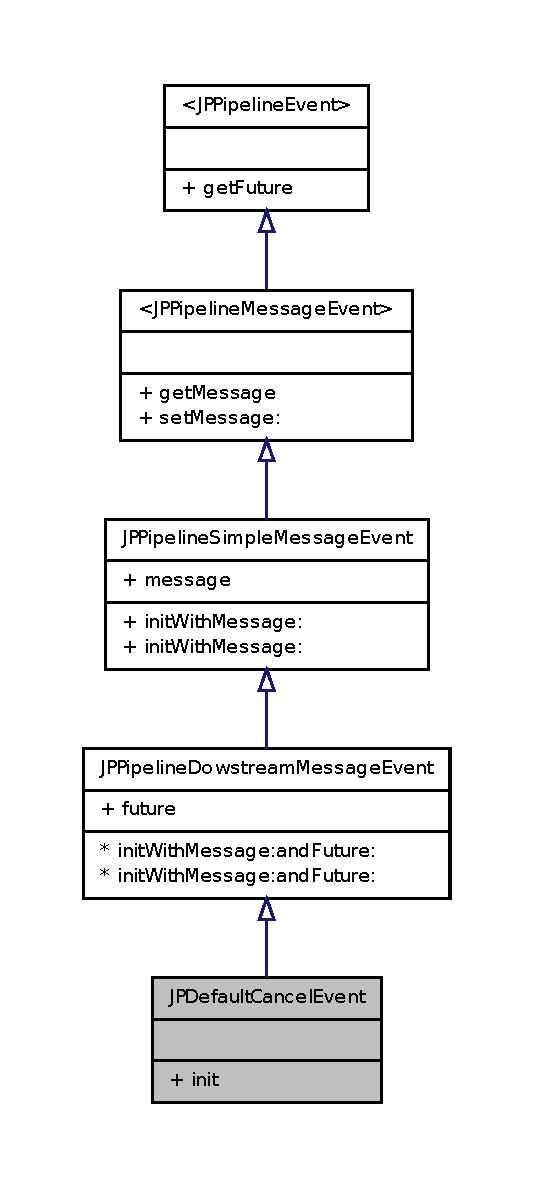
\includegraphics[width=256pt]{a00091}
\end{center}
\end{figure}


Collaboration diagram for JPDefaultCancelEvent:\nopagebreak
\begin{figure}[H]
\begin{center}
\leavevmode
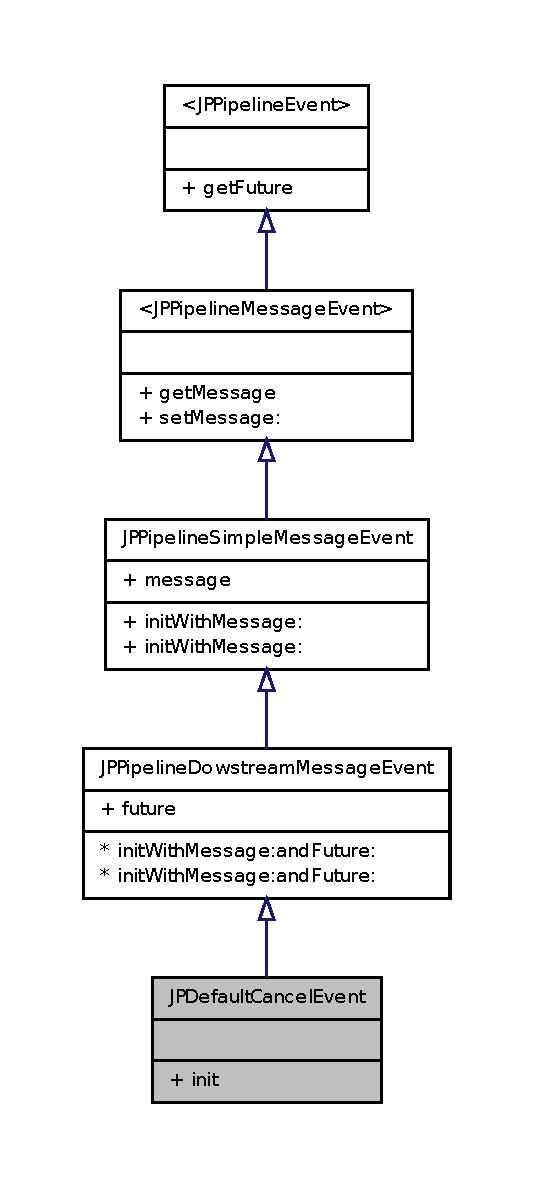
\includegraphics[width=256pt]{a00092}
\end{center}
\end{figure}


\subsection{Detailed Description}
An Pipeline {\bfseries downstream} \hyperlink{a00005}{Event} that represent one {\bfseries \char`\"{}cancel\char`\"{}} action. You can {\bfseries cancel} an {\bfseries downstream} \hyperlink{a00005}{Event} while he is processing sending an \hyperlink{a00010}{JPDefaultCancelEvent} downstream as follow: 
\begin{DoxyCode}
 [pipeline sendDownstream:[JPDefaultCancelEvent init]];
\end{DoxyCode}
 \begin{DoxyNote}{Note}
Instead that \hyperlink{a00001}{The Pipeline} are always an asynchronous I/O operation he process one \hyperlink{a00005}{Event} at a time, that's why you can cancel an event while he is processing or waiting for some answer. 
\end{DoxyNote}


The documentation for this class was generated from the following file:\begin{DoxyCompactItemize}
\item 
/Users/Paulo/Projects/JUMP/JUMPNetwork/Headers/JPDefaultCancelEvent.h\end{DoxyCompactItemize}

\hypertarget{a00011}{
\section{JPDefaultHandlerContext Class Reference}
\label{a00011}\index{JPDefaultHandlerContext@{JPDefaultHandlerContext}}
}


{\ttfamily \#import $<$JPDefaultHandlerContext.h$>$}



Inheritance diagram for JPDefaultHandlerContext:\nopagebreak
\begin{figure}[H]
\begin{center}
\leavevmode
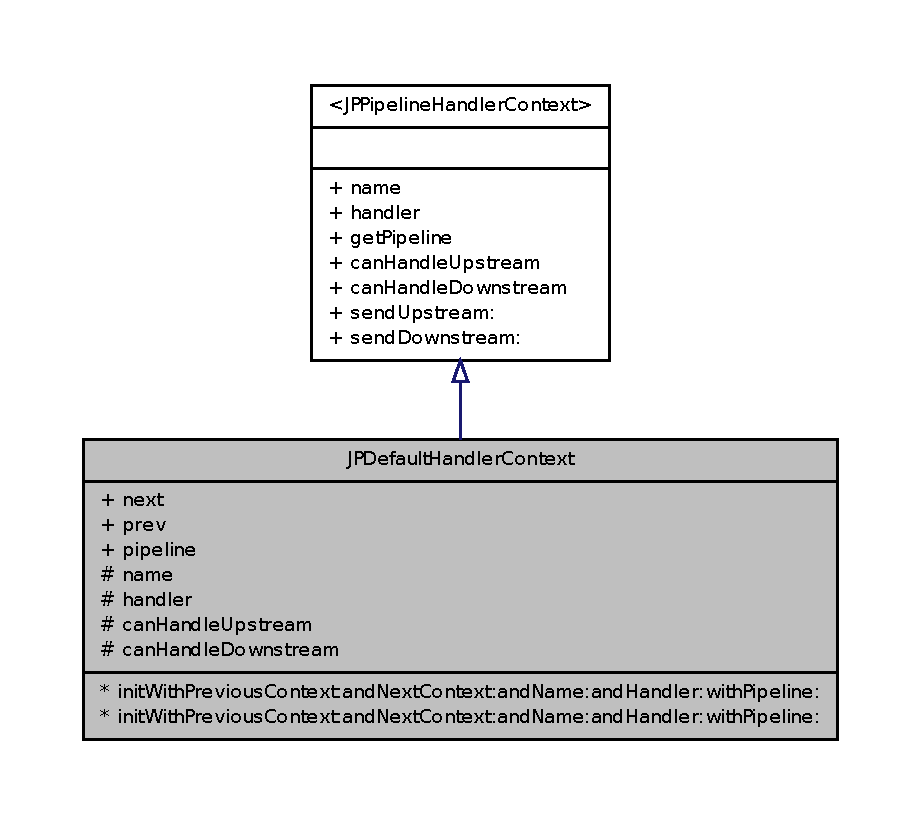
\includegraphics[width=400pt]{a00094}
\end{center}
\end{figure}


Collaboration diagram for JPDefaultHandlerContext:\nopagebreak
\begin{figure}[H]
\begin{center}
\leavevmode
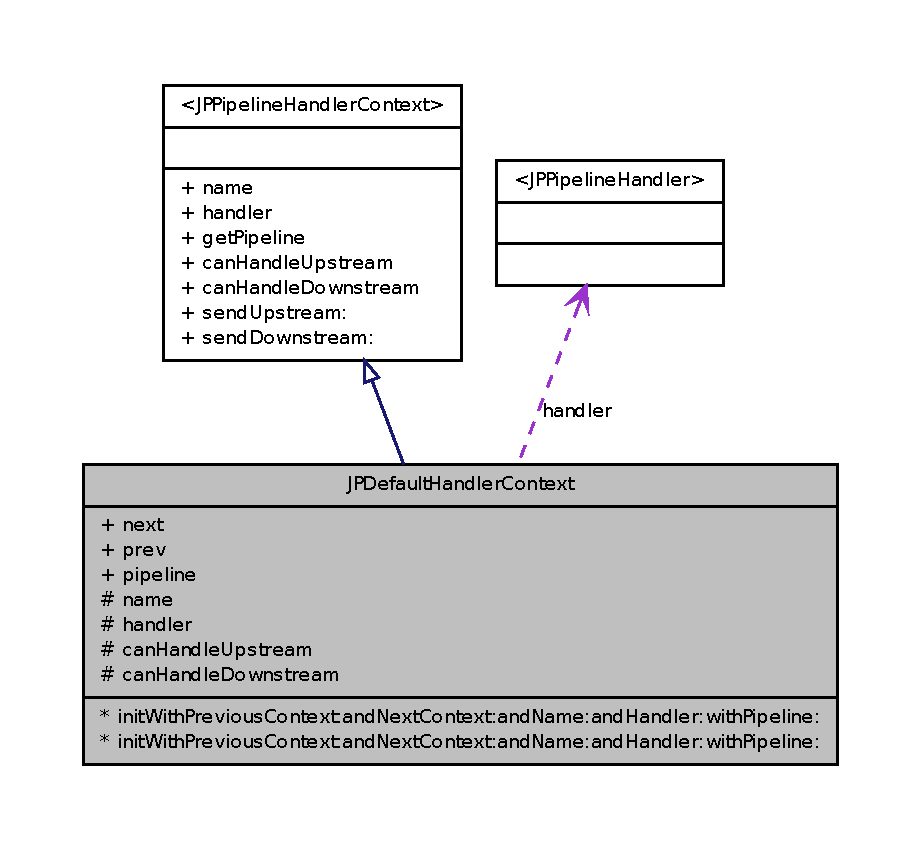
\includegraphics[width=400pt]{a00095}
\end{center}
\end{figure}
\subsection*{Properties}
\begin{DoxyCompactItemize}
\item 
\hypertarget{a00011_a596be5fcf184778f762c26640ac2b36d}{
\hyperlink{a00019}{JPPipeline} $\ast$ \hyperlink{a00011_a596be5fcf184778f762c26640ac2b36d}{pipeline}}
\label{a00011_a596be5fcf184778f762c26640ac2b36d}

\begin{DoxyCompactList}\small\item\em The pipeline this context belong to. \item\end{DoxyCompactList}\end{DoxyCompactItemize}
\subsection*{Init Methods}
\begin{DoxyCompactItemize}
\item 
\hypertarget{a00011_ae0cbf5b65295691aa6c76015fc1ed93c}{
(id) + {\bfseries initWithPreviousContext:andNextContext:andName:andHandler:withPipeline:}}
\label{a00011_ae0cbf5b65295691aa6c76015fc1ed93c}

\item 
\hypertarget{a00011_ae0cbf5b65295691aa6c76015fc1ed93c}{
(id) -\/ {\bfseries initWithPreviousContext:andNextContext:andName:andHandler:withPipeline:}}
\label{a00011_ae0cbf5b65295691aa6c76015fc1ed93c}

\end{DoxyCompactItemize}


\subsection{Detailed Description}
 

The documentation for this class was generated from the following file:\begin{DoxyCompactItemize}
\item 
/Users/Paulo/Projects/JUMP/JUMPNetwork/Headers/JPDefaultHandlerContext.h\end{DoxyCompactItemize}

\hypertarget{a00012}{
\section{JPDefaultHTTPMessage Class Reference}
\label{a00012}\index{JPDefaultHTTPMessage@{JPDefaultHTTPMessage}}
}


\hyperlink{a00012}{JPDefaultHTTPMessage} is an type of \hyperlink{a00006}{Event Message} that encapsulate the HTTP data to be transported.  




{\ttfamily \#import $<$JPDefaultHTTPMessage.h$>$}



Inheritance diagram for JPDefaultHTTPMessage:
\nopagebreak
\begin{figure}[H]
\begin{center}
\leavevmode
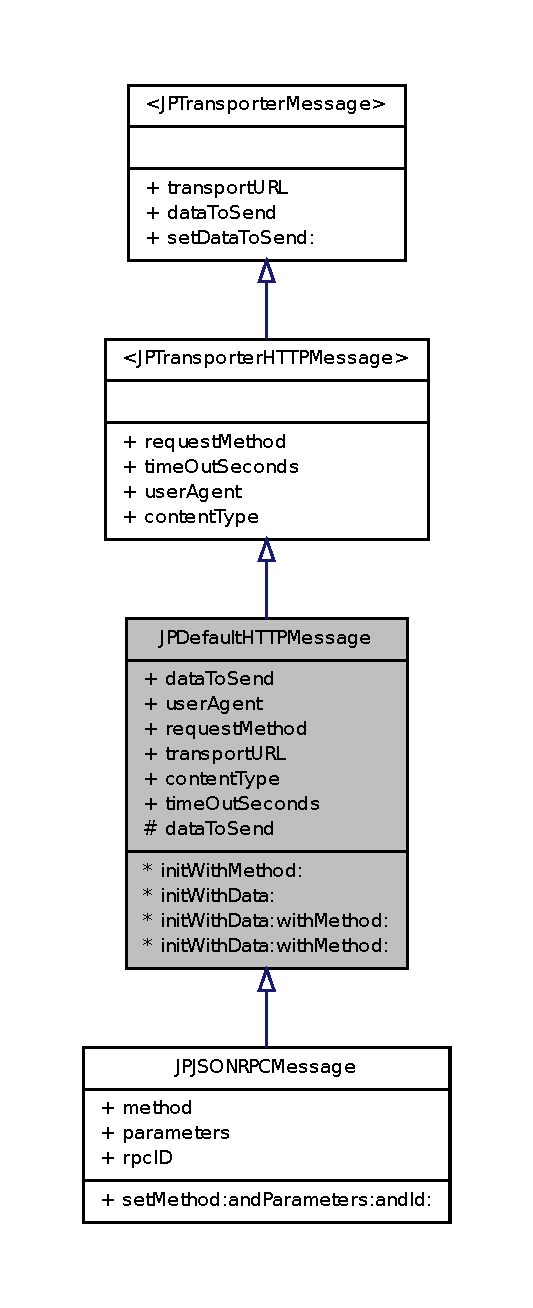
\includegraphics[height=600pt]{a00097}
\end{center}
\end{figure}


Collaboration diagram for JPDefaultHTTPMessage:
\nopagebreak
\begin{figure}[H]
\begin{center}
\leavevmode
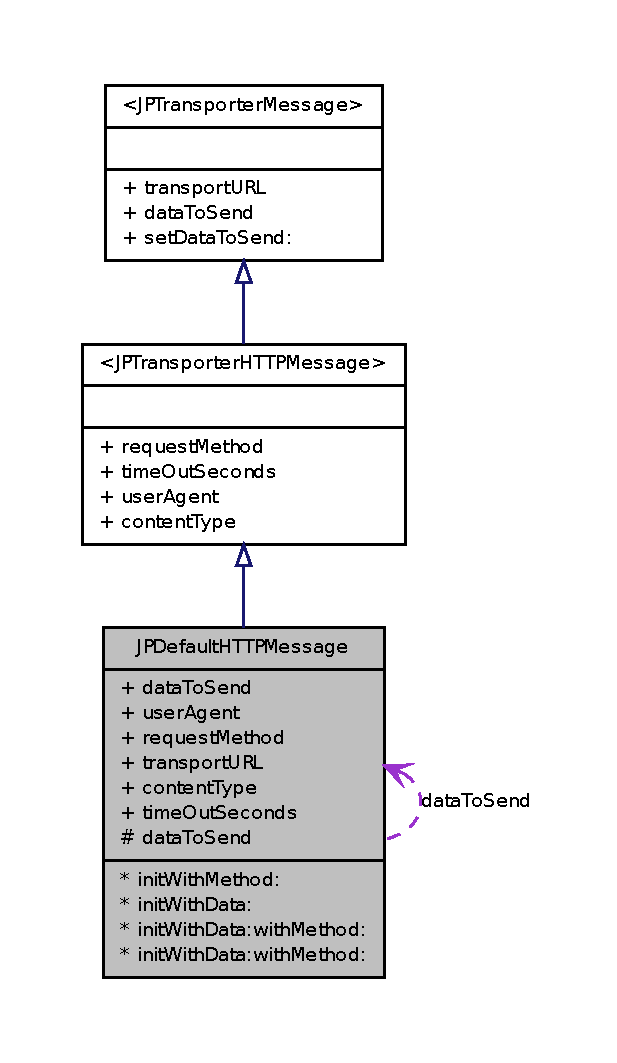
\includegraphics[width=296pt]{a00098}
\end{center}
\end{figure}
\subsection*{Properties}
\begin{DoxyCompactItemize}
\item 
\hypertarget{a00012_aa39bdf65fc26801d45dc3d80cc68892b}{
NSData $\ast$ \hyperlink{a00012_aa39bdf65fc26801d45dc3d80cc68892b}{dataToSend}}
\label{a00012_aa39bdf65fc26801d45dc3d80cc68892b}

\begin{DoxyCompactList}\small\item\em Data that this event transport. \item\end{DoxyCompactList}\item 
\hypertarget{a00012_a3c044d1ed331e62473a3ed37bdeadb30}{
NSString $\ast$ \hyperlink{a00012_a3c044d1ed331e62473a3ed37bdeadb30}{userAgent}}
\label{a00012_a3c044d1ed331e62473a3ed37bdeadb30}

\begin{DoxyCompactList}\small\item\em HTTP User-\/Agent of this message. \item\end{DoxyCompactList}\item 
NSString $\ast$ \hyperlink{a00012_a95ef26b022a5d51a8d5ee34bbbb7e399}{requestMethod}
\begin{DoxyCompactList}\small\item\em HTTP Method of this message. \item\end{DoxyCompactList}\item 
\hypertarget{a00012_a13f97267d17f51149120e5142356ac5c}{
NSURL $\ast$ \hyperlink{a00012_a13f97267d17f51149120e5142356ac5c}{transportURL}}
\label{a00012_a13f97267d17f51149120e5142356ac5c}

\begin{DoxyCompactList}\small\item\em HTTP URL to process this message. \item\end{DoxyCompactList}\item 
NSString $\ast$ \hyperlink{a00012_ac9ab3ce00110b03ae50285c1d5b6e03f}{contentType}
\begin{DoxyCompactList}\small\item\em HTML Content-\/Type of this message. \item\end{DoxyCompactList}\item 
NSTimeInterval \hyperlink{a00012_a47d1d71ffd2145a805f29db0e2dcf5ae}{timeOutSeconds}
\begin{DoxyCompactList}\small\item\em Seconds before timeout this HTTP event. \item\end{DoxyCompactList}\end{DoxyCompactItemize}
\subsection*{Init Methods}
\begin{DoxyCompactItemize}
\item 
(id) + \hyperlink{a00012_a044a72fcfe95de6fe0c7885546e29d5d}{initWithMethod:}
\begin{DoxyCompactList}\small\item\em Init this event with specified Method. \item\end{DoxyCompactList}\item 
(id) + \hyperlink{a00012_a9910f12aba62760010ac09c7295c3a80}{initWithData:}
\begin{DoxyCompactList}\small\item\em Init this event with specified data. \item\end{DoxyCompactList}\item 
(id) + \hyperlink{a00012_abd503576f55ca76517961c74b99815ef}{initWithData:withMethod:}
\begin{DoxyCompactList}\small\item\em Init this event with specified data and an HTTP Method. \item\end{DoxyCompactList}\item 
\hypertarget{a00012_abd503576f55ca76517961c74b99815ef}{
(id) -\/ {\bfseries initWithData:withMethod:}}
\label{a00012_abd503576f55ca76517961c74b99815ef}

\end{DoxyCompactItemize}


\subsection{Detailed Description}
\hyperlink{a00012}{JPDefaultHTTPMessage} is an type of \hyperlink{a00006}{Event Message} that encapsulate the HTTP data to be transported. \hyperlink{a00012}{JPDefaultHTTPMessage} is an implementaton of the \hyperlink{a00040}{JPTransporterHTTPMessage} protocol. It is an type of \hyperlink{a00006}{Event Message} that encapsulate the HTTP data to be transported by the \hyperlink{a00014}{JPHTTPTransporter} \hyperlink{a00002}{I$|$O implementation}. You can use this class directly, create your own subclass of this event or create your own implementation of the \hyperlink{a00040}{JPTransporterHTTPMessage} protocol. 

An simply code to illustrate how to send an \hyperlink{a00012}{JPDefaultHTTPMessage} downstream: 
\begin{DoxyCode}
 JPDefaultHTTPMessage *eventMessage = [JPDefaultHTTPMessage initWithData:dataToTr
      ansport withMethod:@"POST"]
 eventMessage.transportURL = [NSURL URLWithString:@"http://seqoy.org/httpgateway"
      ];
 
 [pipeline sendDownstream:[JPPipelineMessageEvent initWithMessage:eventMessage]];
      
\end{DoxyCode}
 Of course this example require a big boilerplate for a simple operation. See \hyperlink{a00004}{Using Factories} for more information to how configure and automate boilerplates using \href{http://en.wikipedia.org/wiki/Factory_method_pattern}{\tt Factory Patterns}.

\subsubsection*{Additional resources worth reading}

See \hyperlink{a00008}{JSON-\/RPC Event Messages} to learn about \hyperlink{a00006}{Event Message} that use HTTP components as basis.

\par
 \par
 

\subsection{Member Function Documentation}
\hypertarget{a00012_a044a72fcfe95de6fe0c7885546e29d5d}{
\index{JPDefaultHTTPMessage@{JPDefaultHTTPMessage}!initWithMethod:@{initWithMethod:}}
\index{initWithMethod:@{initWithMethod:}!JPDefaultHTTPMessage@{JPDefaultHTTPMessage}}
\subsubsection[{initWithMethod:}]{\setlength{\rightskip}{0pt plus 5cm}+ (id) initWithMethod: 
\begin{DoxyParamCaption}
\item[{dummy(NSString $\ast$)}]{anMethod}
\end{DoxyParamCaption}
}}
\label{a00012_a044a72fcfe95de6fe0c7885546e29d5d}


Init this event with specified Method. 


\begin{DoxyParams}{Parameters}
{\em anMethod} & HTTP Method of this message. \\
\hline
\end{DoxyParams}
\hypertarget{a00012_a9910f12aba62760010ac09c7295c3a80}{
\index{JPDefaultHTTPMessage@{JPDefaultHTTPMessage}!initWithData:@{initWithData:}}
\index{initWithData:@{initWithData:}!JPDefaultHTTPMessage@{JPDefaultHTTPMessage}}
\subsubsection[{initWithData:}]{\setlength{\rightskip}{0pt plus 5cm}+ (id) initWithData: 
\begin{DoxyParamCaption}
\item[{dummy(NSData $\ast$)}]{anData}
\end{DoxyParamCaption}
}}
\label{a00012_a9910f12aba62760010ac09c7295c3a80}


Init this event with specified data. 


\begin{DoxyParams}{Parameters}
{\em anData} & Data that this event transport. \\
\hline
\end{DoxyParams}
\hypertarget{a00012_abd503576f55ca76517961c74b99815ef}{
\index{JPDefaultHTTPMessage@{JPDefaultHTTPMessage}!initWithData:withMethod:@{initWithData:withMethod:}}
\index{initWithData:withMethod:@{initWithData:withMethod:}!JPDefaultHTTPMessage@{JPDefaultHTTPMessage}}
\subsubsection[{initWithData:withMethod:}]{\setlength{\rightskip}{0pt plus 5cm}+ (id) initWithData: 
\begin{DoxyParamCaption}
\item[{dummy(NSData $\ast$)}]{anData}
\item[{withMethod:(NSString $\ast$)}]{anMethod}
\end{DoxyParamCaption}
}}
\label{a00012_abd503576f55ca76517961c74b99815ef}


Init this event with specified data and an HTTP Method. 


\begin{DoxyParams}{Parameters}
{\em anData} & Data that this event transport. \\
\hline
{\em anMethod} & HTTP Method of this message. \\
\hline
\end{DoxyParams}


\subsection{Property Documentation}
\hypertarget{a00012_a95ef26b022a5d51a8d5ee34bbbb7e399}{
\index{JPDefaultHTTPMessage@{JPDefaultHTTPMessage}!requestMethod@{requestMethod}}
\index{requestMethod@{requestMethod}!JPDefaultHTTPMessage@{JPDefaultHTTPMessage}}
\subsubsection[{requestMethod}]{\setlength{\rightskip}{0pt plus 5cm}-\/ (NSString $\ast$) requestMethod\hspace{0.3cm}{\ttfamily  \mbox{[}read, write, copy\mbox{]}}}}
\label{a00012_a95ef26b022a5d51a8d5ee34bbbb7e399}


HTTP Method of this message. 

Default value is {\bfseries \char`\"{}POST\char`\"{}}. \hypertarget{a00012_ac9ab3ce00110b03ae50285c1d5b6e03f}{
\index{JPDefaultHTTPMessage@{JPDefaultHTTPMessage}!contentType@{contentType}}
\index{contentType@{contentType}!JPDefaultHTTPMessage@{JPDefaultHTTPMessage}}
\subsubsection[{contentType}]{\setlength{\rightskip}{0pt plus 5cm}-\/ (NSString $\ast$) contentType\hspace{0.3cm}{\ttfamily  \mbox{[}read, write, copy\mbox{]}}}}
\label{a00012_ac9ab3ce00110b03ae50285c1d5b6e03f}


HTML Content-\/Type of this message. 

Default value is {\bfseries \char`\"{}text/plain\char`\"{}}. \hypertarget{a00012_a47d1d71ffd2145a805f29db0e2dcf5ae}{
\index{JPDefaultHTTPMessage@{JPDefaultHTTPMessage}!timeOutSeconds@{timeOutSeconds}}
\index{timeOutSeconds@{timeOutSeconds}!JPDefaultHTTPMessage@{JPDefaultHTTPMessage}}
\subsubsection[{timeOutSeconds}]{\setlength{\rightskip}{0pt plus 5cm}-\/ (NSTimeInterval) timeOutSeconds\hspace{0.3cm}{\ttfamily  \mbox{[}read, write, assign\mbox{]}}}}
\label{a00012_a47d1d71ffd2145a805f29db0e2dcf5ae}


Seconds before timeout this HTTP event. 

Default value is {\bfseries 300 seconds (5 minutes)}. 

The documentation for this class was generated from the following file:\begin{DoxyCompactItemize}
\item 
/Users/Paulo/Projects/JUMP/JUMPNetwork/Headers/JPDefaultHTTPMessage.h\end{DoxyCompactItemize}

\hypertarget{a00013}{
\section{JPDefaultPipelineExceptionEvent Class Reference}
\label{a00013}\index{JPDefaultPipelineExceptionEvent@{JPDefaultPipelineExceptionEvent}}
}


The default Pipeline Exception Event implementation.  




{\ttfamily \#import $<$JPDefaultPipelineExceptionEvent.h$>$}



Inheritance diagram for JPDefaultPipelineExceptionEvent:\nopagebreak
\begin{figure}[H]
\begin{center}
\leavevmode
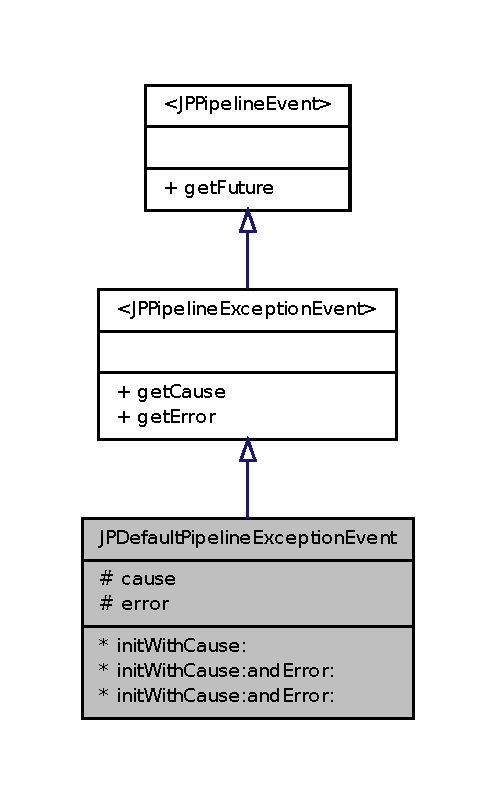
\includegraphics[width=238pt]{a00100}
\end{center}
\end{figure}


Collaboration diagram for JPDefaultPipelineExceptionEvent:\nopagebreak
\begin{figure}[H]
\begin{center}
\leavevmode
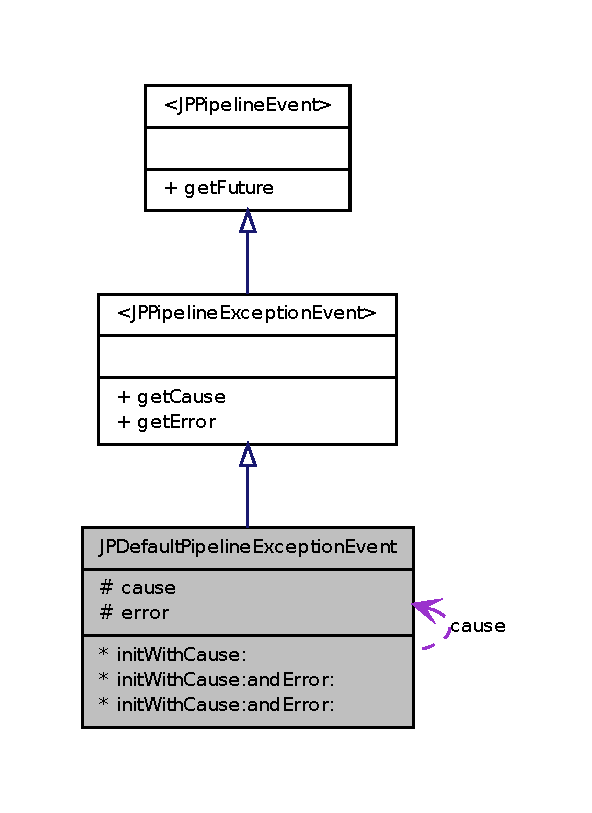
\includegraphics[width=284pt]{a00101}
\end{center}
\end{figure}
\subsection*{Init Methods}
\begin{DoxyCompactItemize}
\item 
(id) + \hyperlink{a00013_a75373c54d3c579331c6e08f133ef06f3}{initWithCause:}
\begin{DoxyCompactList}\small\item\em Init the event with an cause. \item\end{DoxyCompactList}\item 
(id) + \hyperlink{a00013_a9d2e38b2c6c789a9b94b6e5be50746d0}{initWithCause:andError:}
\begin{DoxyCompactList}\small\item\em Init the event with an cause. \item\end{DoxyCompactList}\item 
\hypertarget{a00013_a9d2e38b2c6c789a9b94b6e5be50746d0}{
(id) -\/ {\bfseries initWithCause:andError:}}
\label{a00013_a9d2e38b2c6c789a9b94b6e5be50746d0}

\end{DoxyCompactItemize}


\subsection{Detailed Description}
The default Pipeline Exception Event implementation. 

\subsection{Member Function Documentation}
\hypertarget{a00013_a75373c54d3c579331c6e08f133ef06f3}{
\index{JPDefaultPipelineExceptionEvent@{JPDefaultPipelineExceptionEvent}!initWithCause:@{initWithCause:}}
\index{initWithCause:@{initWithCause:}!JPDefaultPipelineExceptionEvent@{JPDefaultPipelineExceptionEvent}}
\subsubsection[{initWithCause:}]{\setlength{\rightskip}{0pt plus 5cm}+ (id) initWithCause: 
\begin{DoxyParamCaption}
\item[{dummy(NSException $\ast$)}]{anCause}
\end{DoxyParamCaption}
}}
\label{a00013_a75373c54d3c579331c6e08f133ef06f3}


Init the event with an cause. 


\begin{DoxyParams}{Parameters}
{\em anCause} & An exception object that represent the cause of this Exception. \\
\hline
\end{DoxyParams}
\hypertarget{a00013_a9d2e38b2c6c789a9b94b6e5be50746d0}{
\index{JPDefaultPipelineExceptionEvent@{JPDefaultPipelineExceptionEvent}!initWithCause:andError:@{initWithCause:andError:}}
\index{initWithCause:andError:@{initWithCause:andError:}!JPDefaultPipelineExceptionEvent@{JPDefaultPipelineExceptionEvent}}
\subsubsection[{initWithCause:andError:}]{\setlength{\rightskip}{0pt plus 5cm}+ (id) initWithCause: 
\begin{DoxyParamCaption}
\item[{dummy(NSException $\ast$)}]{anCause}
\item[{andError:(NSError $\ast$)}]{anError}
\end{DoxyParamCaption}
}}
\label{a00013_a9d2e38b2c6c789a9b94b6e5be50746d0}


Init the event with an cause. 


\begin{DoxyParams}{Parameters}
{\em anCause} & An exception object that represent the cause of this Exception. \\
\hline
{\em anError} & An error object that represent the cause of this Exception. \\
\hline
\end{DoxyParams}


The documentation for this class was generated from the following file:\begin{DoxyCompactItemize}
\item 
/Users/Paulo/Projects/JUMP/JUMPNetwork/Headers/JPDefaultPipelineExceptionEvent.h\end{DoxyCompactItemize}

\hypertarget{a00014}{
\section{JPHTTPTransporter Class Reference}
\label{a00014}\index{JPHTTPTransporter@{JPHTTPTransporter}}
}


An default {\bfseries HTTP} implementation of the \hyperlink{a00002}{I$|$O Transporter} that conforms with the \hyperlink{a00034}{JPPipelineSink} protocol.  




{\ttfamily \#import $<$JPHTTPTransporter.h$>$}



Inheritance diagram for JPHTTPTransporter:\nopagebreak
\begin{figure}[H]
\begin{center}
\leavevmode
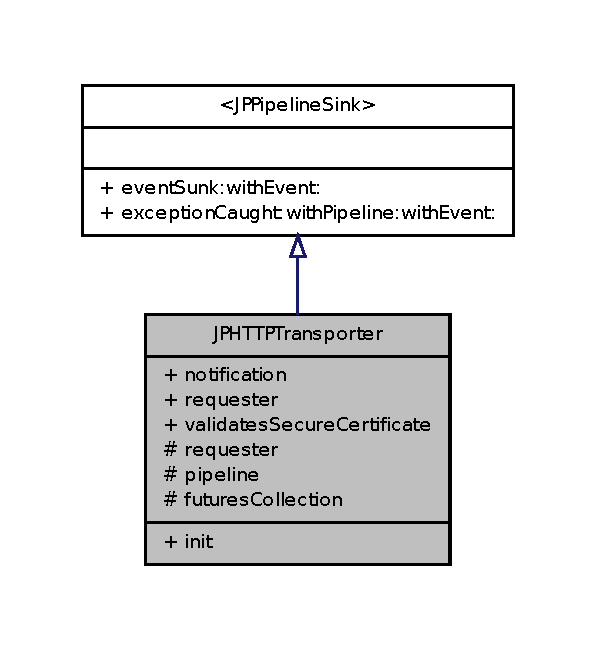
\includegraphics[width=286pt]{a00103}
\end{center}
\end{figure}


Collaboration diagram for JPHTTPTransporter:\nopagebreak
\begin{figure}[H]
\begin{center}
\leavevmode
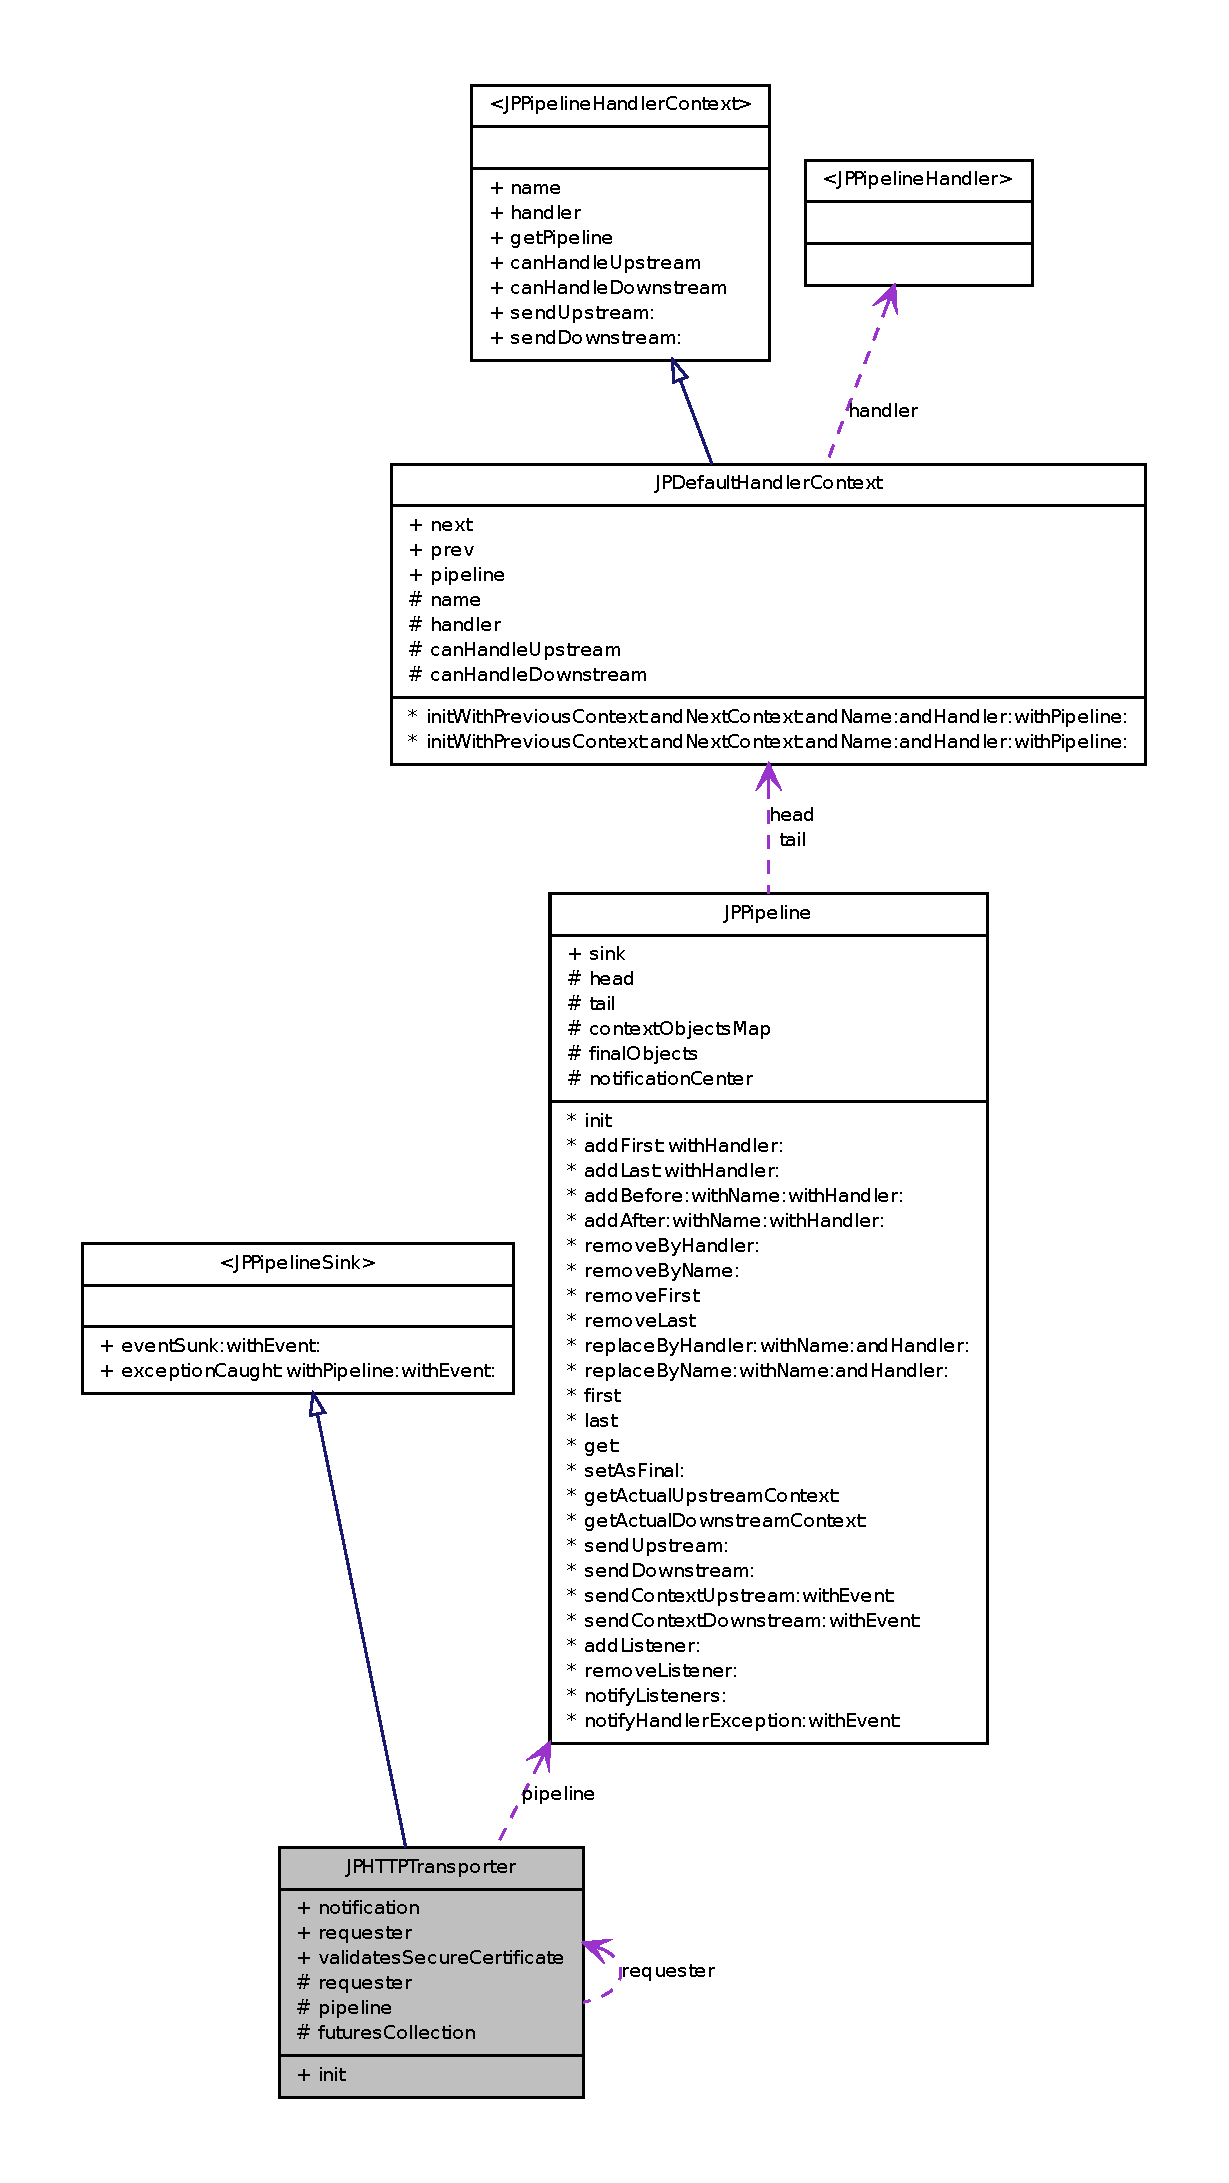
\includegraphics[height=600pt]{a00104}
\end{center}
\end{figure}
\subsection*{Properties}
\begin{DoxyCompactItemize}
\item 
\hypertarget{a00014_a290cddab6355f93ad3d3925497459fc0}{
\hyperlink{a00032}{JPPipelineNotification} $\ast$ \hyperlink{a00014_a290cddab6355f93ad3d3925497459fc0}{notification}}
\label{a00014_a290cddab6355f93ad3d3925497459fc0}

\begin{DoxyCompactList}\small\item\em Pipeline Notification. \item\end{DoxyCompactList}\item 
\hypertarget{a00014_aec61cceb936f46d429b52d312f0caa09}{
ASIHTTPRequest $\ast$ \hyperlink{a00014_aec61cceb936f46d429b52d312f0caa09}{requester}}
\label{a00014_aec61cceb936f46d429b52d312f0caa09}

\begin{DoxyCompactList}\small\item\em The HTTP Requester. \item\end{DoxyCompactList}\item 
\hypertarget{a00014_a9b5dd41765aa7e924f9906189a8d56fc}{
BOOL \hyperlink{a00014_a9b5dd41765aa7e924f9906189a8d56fc}{validatesSecureCertificate}}
\label{a00014_a9b5dd41765aa7e924f9906189a8d56fc}

\begin{DoxyCompactList}\small\item\em Should validate any Security Certificate. \item\end{DoxyCompactList}\end{DoxyCompactItemize}


\subsection{Detailed Description}
An default {\bfseries HTTP} implementation of the \hyperlink{a00002}{I$|$O Transporter} that conforms with the \hyperlink{a00034}{JPPipelineSink} protocol. This default implementation use the \href{http://es.wikipedia.org/wiki/Hypertext_Transfer_Protocol}{\tt HTTP protocol} to transport data between an external server and your application, performing basic HTTP requests and interacting with REST-\/based services (GET / POST / PUT / DELETE). 

Internally it uses the wonderful \href{http://allseeing-i.com/ASIHTTPRequest/}{\tt ASIHTTPRequest} library. {\bfseries ASIHTTPRequest} is builded on top of the \href{http://developer.apple.com/library/mac/#documentation/Networking/Conceptual/CFNetwork/Introduction/Introduction.html}{\tt Apple CFNetwork API} and works in both Mac OS X and iPhone applications. 

Once created your \hyperlink{a00019}{JPPipeline} you should attach the transporter. 
\begin{DoxyCode}
 // Create new Pipeline.
 JPPipeline *pipeline = [JPPipeline init];
 
 // HTTP Transporter associated with the pipeline.
 pipeline.sink = [JPHTTPTransporter init];
\end{DoxyCode}
 \subsubsection*{HTTP Transporter Events Messages}

\hyperlink{a00012}{JPDefaultHTTPMessage} is an implementaton of the \hyperlink{a00040}{JPTransporterHTTPMessage} protocol. It is an type of \hyperlink{a00006}{Event Message} that encapsulate the HTTP data to be transported by the \hyperlink{a00014}{JPHTTPTransporter} \hyperlink{a00002}{I$|$O implementation}. You can use this class directly, create your own subclass of this event or create your own implementation of the \hyperlink{a00040}{JPTransporterHTTPMessage} protocol. 

An simply code to illustrate how to send an \hyperlink{a00012}{JPDefaultHTTPMessage} downstream: 
\begin{DoxyCode}
 JPDefaultHTTPMessage *eventMessage = [JPDefaultHTTPMessage initWithData:dataToTr
      ansport withMethod:@"POST"]
 eventMessage.transportURL = [NSURL URLWithString:@"http://seqoy.org/httpgateway"
      ];
 
 [pipeline sendDownstream:[JPPipelineMessageEvent initWithMessage:eventMessage]];
      
\end{DoxyCode}
 Of course this example require a big boilerplate for a simple operation. See \hyperlink{a00004}{Using Factories} for more information to how configure and automate boilerplates using \href{http://en.wikipedia.org/wiki/Factory_method_pattern}{\tt Factory Patterns}.

\subsubsection*{Additional resources worth reading}

See \hyperlink{a00008}{JSON-\/RPC Event Messages} to learn about \hyperlink{a00006}{Event Message} that use HTTP components as basis.

\par
 \par
  

The documentation for this class was generated from the following file:\begin{DoxyCompactItemize}
\item 
/Users/Paulo/Projects/JUMP/JUMPNetwork/Headers/JPHTTPTransporter.h\end{DoxyCompactItemize}

\hypertarget{a00015}{
\section{JPJSONRPCDecoderHandler Class Reference}
\label{a00015}\index{JPJSONRPCDecoderHandler@{JPJSONRPCDecoderHandler}}
}


An simple JSON-\/RPC Decoder Handler.  




{\ttfamily \#import $<$JPJSONRPCDecoderHandler.h$>$}



Inheritance diagram for JPJSONRPCDecoderHandler:\nopagebreak
\begin{figure}[H]
\begin{center}
\leavevmode
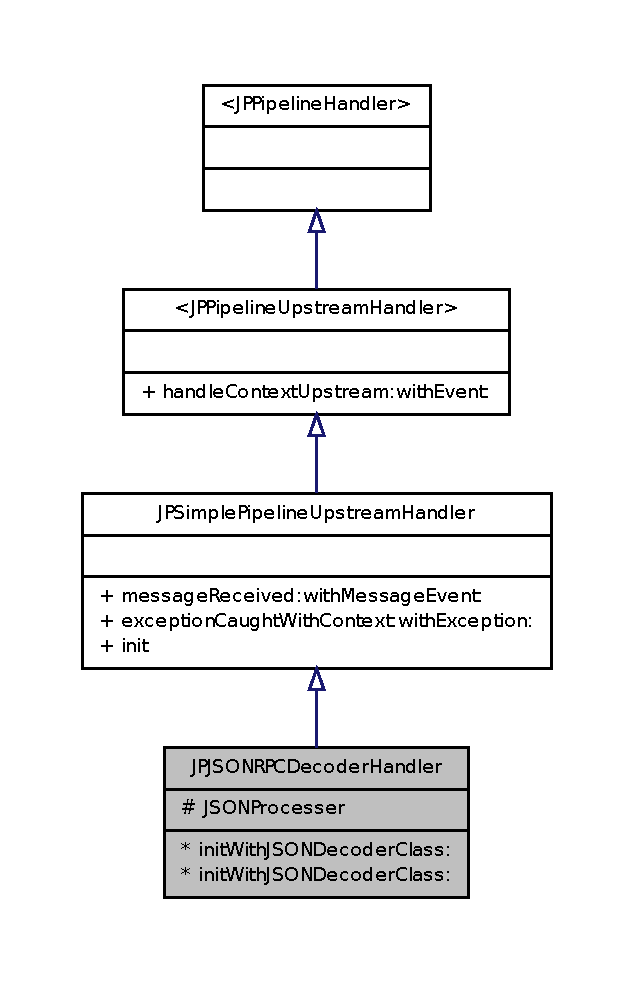
\includegraphics[width=304pt]{a00106}
\end{center}
\end{figure}


Collaboration diagram for JPJSONRPCDecoderHandler:\nopagebreak
\begin{figure}[H]
\begin{center}
\leavevmode
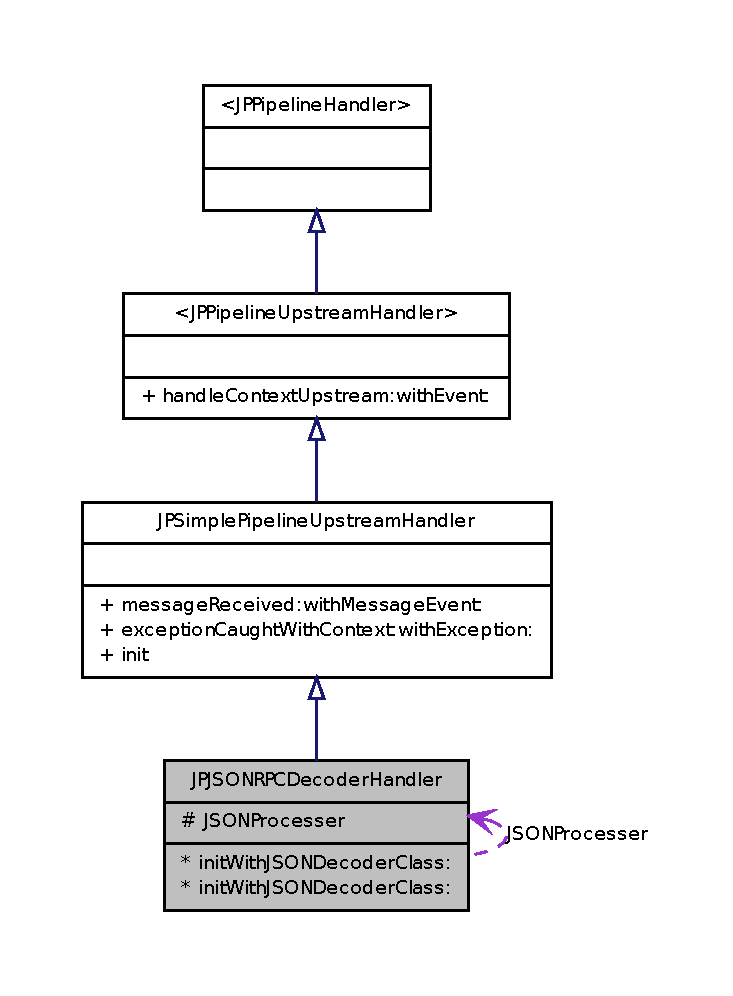
\includegraphics[width=352pt]{a00107}
\end{center}
\end{figure}
\subsection*{Protected Types}
\begin{DoxyCompactItemize}
\item 
enum \hyperlink{a00015_aba2b766c1b7742f5c636bbbd578df618}{JPJSONRPCDecoderErrors} \{ \hyperlink{a00015_aba2b766c1b7742f5c636bbbd578df618adaa30b18406ba5a080ea1dddc621b154}{kJSONRPCCantDecode}, 
\hyperlink{a00015_aba2b766c1b7742f5c636bbbd578df618a2500b118aeb7e1f2d305c9edaa6e3376}{kJSONRPCInvalid}
 \}
\end{DoxyCompactItemize}
\subsection*{Init Methods}
\begin{DoxyCompactItemize}
\item 
(id) + \hyperlink{a00015_a35ae826d8a4a5a44ffc17ed495b97bee}{initWithJSONDecoderClass:}
\begin{DoxyCompactList}\small\item\em Init the JSON Decoder Handler. \item\end{DoxyCompactList}\item 
\hypertarget{a00015_a35ae826d8a4a5a44ffc17ed495b97bee}{
(id) -\/ {\bfseries initWithJSONDecoderClass:}}
\label{a00015_a35ae826d8a4a5a44ffc17ed495b97bee}

\end{DoxyCompactItemize}


\subsection{Detailed Description}
An simple JSON-\/RPC Decoder Handler. \hyperlink{a00015}{JPJSONRPCDecoderHandler} intercepts any {\bfseries upstream} \hyperlink{a00006}{Event Message} and try to decode as a {\bfseries JSON Object} first, and then to interpret the JSON-\/RPC properties. 

If \hyperlink{a00015}{JPJSONRPCDecoderHandler} can't decode to JSON Object or can't found the RPC properties will send an \hyperlink{a00013}{JPDefaultPipelineExceptionEvent} upstream as a warning error, you can catch this exception and process it as an decode error. Refer to \hyperlink{a00015_aba2b766c1b7742f5c636bbbd578df618}{JPJSONRPCDecoderErrors} to known the proper {\bfseries error code}. 

You also can ignore this exception and let the next handler (if exist) continue the processing, because the unmodified \hyperlink{a00006}{Event Message} are sent upstream to the next handler even when an error ocurrs. This is useful if you have an \hyperlink{a00001}{pipeline} that decode differents types of \hyperlink{a00006}{Event Message} ({\itshape e.g. XML and JSON\/}) at the same time. 

Here an example that how you assign the \hyperlink{a00015}{JPJSONRPCDecoderHandler} to the pipeline: 
\begin{DoxyCode}
 [pipeline addLast:@"JSONRPCDecoder" withHandler:[JPJSONRPCDecoderHandler initWit
      hJSONDecoderClass:[JSONEncoder class]]];
\end{DoxyCode}
 The \hyperlink{a00015}{JPJSONRPCDecoderHandler} doesn't have an embedded JSON Decoder. You have to inform one JSON Processer Class that conform with the \hyperlink{a00009}{JPDataProcessserJSON} protocol. See the {\bfseries JUMP Data Module} to find an default implementation of this protocol that you can use or you can implement your own. 

\subsection{Member Enumeration Documentation}
\hypertarget{a00015_aba2b766c1b7742f5c636bbbd578df618}{
\index{JPJSONRPCDecoderHandler@{JPJSONRPCDecoderHandler}!JPJSONRPCDecoderErrors@{JPJSONRPCDecoderErrors}}
\index{JPJSONRPCDecoderErrors@{JPJSONRPCDecoderErrors}!JPJSONRPCDecoderHandler@{JPJSONRPCDecoderHandler}}
\subsubsection[{JPJSONRPCDecoderErrors}]{\setlength{\rightskip}{0pt plus 5cm}-\/ (enum) {\bf JPJSONRPCDecoderErrors}\hspace{0.3cm}{\ttfamily  \mbox{[}protected\mbox{]}}}}
\label{a00015_aba2b766c1b7742f5c636bbbd578df618}
Default JSON-\/RPC Decoder Errors. You can use this errors codes when you are retrieving some exception from the pipeline. Look for the {\ttfamily 'JPJSONRPCDecoderHandler'} domain an some of this errors constants. \begin{Desc}
\item[Enumerator: ]\par
\begin{description}
\index{kJSONRPCCantDecode@{kJSONRPCCantDecode}!JPJSONRPCDecoderHandler@{JPJSONRPCDecoderHandler}}\index{JPJSONRPCDecoderHandler@{JPJSONRPCDecoderHandler}!kJSONRPCCantDecode@{kJSONRPCCantDecode}}\item[{\em 
\hypertarget{a00015_aba2b766c1b7742f5c636bbbd578df618adaa30b18406ba5a080ea1dddc621b154}{
kJSONRPCCantDecode}
\label{a00015_aba2b766c1b7742f5c636bbbd578df618adaa30b18406ba5a080ea1dddc621b154}
}]Can't decode the Response String as JSON Object. Probably isn't an JSON String or is invalid. \index{kJSONRPCInvalid@{kJSONRPCInvalid}!JPJSONRPCDecoderHandler@{JPJSONRPCDecoderHandler}}\index{JPJSONRPCDecoderHandler@{JPJSONRPCDecoderHandler}!kJSONRPCInvalid@{kJSONRPCInvalid}}\item[{\em 
\hypertarget{a00015_aba2b766c1b7742f5c636bbbd578df618a2500b118aeb7e1f2d305c9edaa6e3376}{
kJSONRPCInvalid}
\label{a00015_aba2b766c1b7742f5c636bbbd578df618a2500b118aeb7e1f2d305c9edaa6e3376}
}]Invalid JSON-\/RPC data. Is an correct JSON String, but invalid RPC format. \end{description}
\end{Desc}



\subsection{Member Function Documentation}
\hypertarget{a00015_a35ae826d8a4a5a44ffc17ed495b97bee}{
\index{JPJSONRPCDecoderHandler@{JPJSONRPCDecoderHandler}!initWithJSONDecoderClass:@{initWithJSONDecoderClass:}}
\index{initWithJSONDecoderClass:@{initWithJSONDecoderClass:}!JPJSONRPCDecoderHandler@{JPJSONRPCDecoderHandler}}
\subsubsection[{initWithJSONDecoderClass:}]{\setlength{\rightskip}{0pt plus 5cm}+ (id) initWithJSONDecoderClass: 
\begin{DoxyParamCaption}
\item[{dummy(Class$<$ {\bf JPDataProcessserJSON} $>$)}]{anJSONProcesserClass}
\end{DoxyParamCaption}
}}
\label{a00015_a35ae826d8a4a5a44ffc17ed495b97bee}


Init the JSON Decoder Handler. 


\begin{DoxyParams}{Parameters}
{\em anJSONProcesserClass} & A {\ttfamily Class} of an custom JSON Processer that conforms with the \hyperlink{a00009}{JPDataProcessserJSON} protocol. \\
\hline
\end{DoxyParams}


The documentation for this class was generated from the following file:\begin{DoxyCompactItemize}
\item 
/Users/Paulo/Projects/JUMP/JUMPNetwork/Headers/JPJSONRPCDecoderHandler.h\end{DoxyCompactItemize}

\hypertarget{a00016}{
\section{JPJSONRPCEncoderHandler Class Reference}
\label{a00016}\index{JPJSONRPCEncoderHandler@{JPJSONRPCEncoderHandler}}
}


An simple JSON-\/RPC Encoder Handler.  




{\ttfamily \#import $<$JPJSONRPCEncoderHandler.h$>$}



Inheritance diagram for JPJSONRPCEncoderHandler:\nopagebreak
\begin{figure}[H]
\begin{center}
\leavevmode
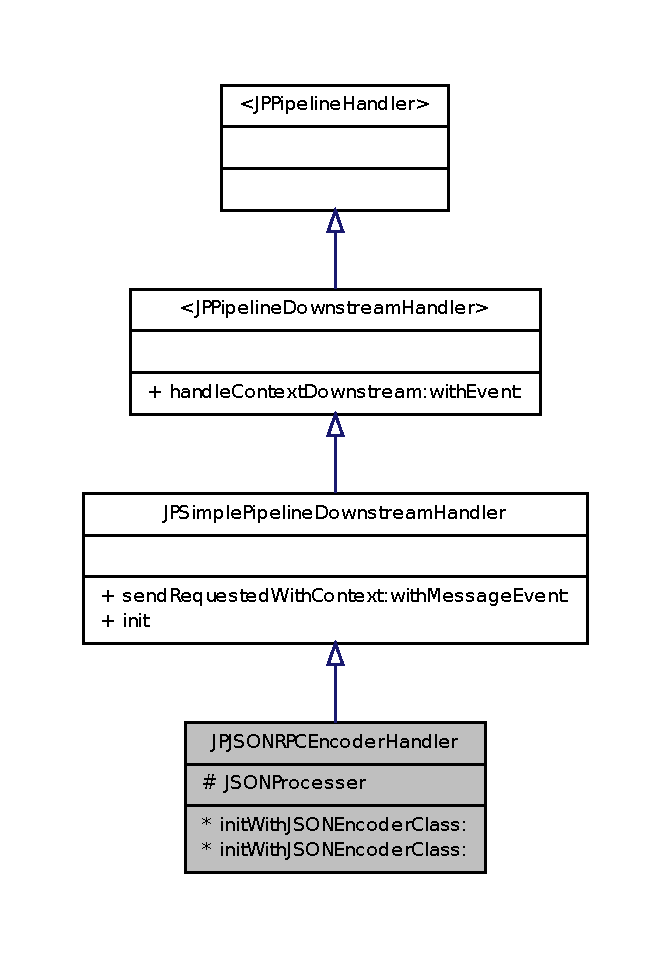
\includegraphics[width=322pt]{a00109}
\end{center}
\end{figure}


Collaboration diagram for JPJSONRPCEncoderHandler:\nopagebreak
\begin{figure}[H]
\begin{center}
\leavevmode
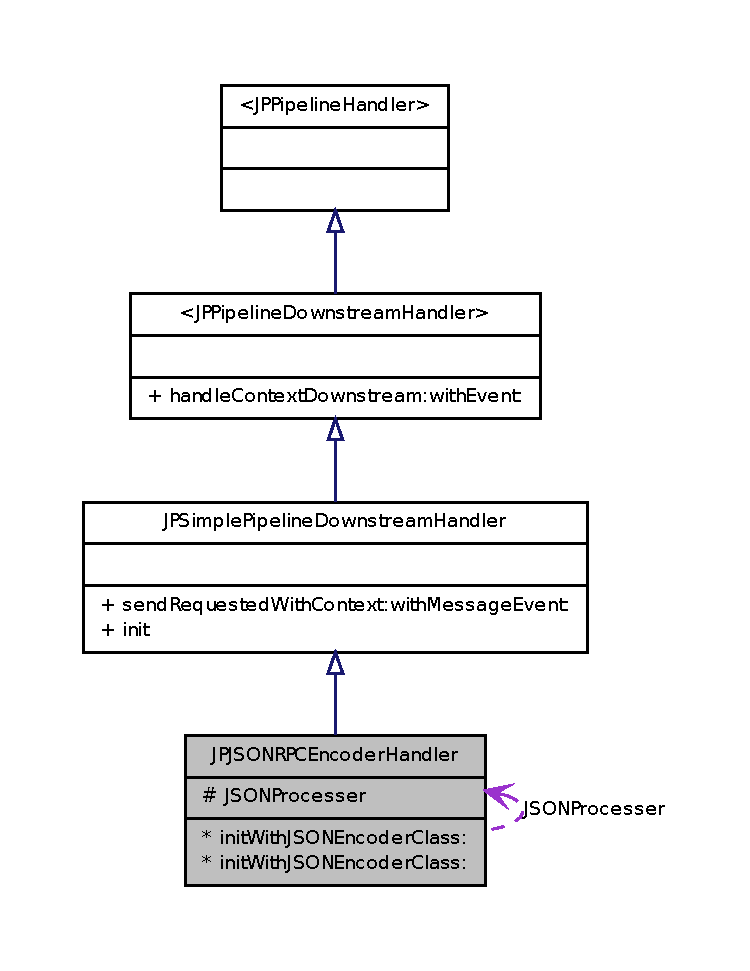
\includegraphics[width=360pt]{a00110}
\end{center}
\end{figure}
\subsection*{Init Methods}
\begin{DoxyCompactItemize}
\item 
(id) + \hyperlink{a00016_ac232419eba6d5ad305b0412e92945dab}{initWithJSONEncoderClass:}
\begin{DoxyCompactList}\small\item\em Init the JSON Encoder Handler. \item\end{DoxyCompactList}\item 
\hypertarget{a00016_ac232419eba6d5ad305b0412e92945dab}{
(id) -\/ {\bfseries initWithJSONEncoderClass:}}
\label{a00016_ac232419eba6d5ad305b0412e92945dab}

\end{DoxyCompactItemize}


\subsection{Detailed Description}
An simple JSON-\/RPC Encoder Handler. \hyperlink{a00016}{JPJSONRPCEncoderHandler} intercepts {\bfseries downstream} \hyperlink{a00018}{JPJSONRPCMessage} and encode his RPC properties, fisrt on a JSON String and later on {\bfseries NSData} to be sent by a \hyperlink{a00002}{I$|$O Transporter}. Other types of messages are ignored and sented downstream to the next handler on the \hyperlink{a00001}{The Pipeline}. 

Here an example that how you assign the \hyperlink{a00016}{JPJSONRPCEncoderHandler} to the pipeline: 
\begin{DoxyCode}
 [pipeline addLast:@"JSONRPCEncoder" withHandler:[JPJSONRPCEncoderHandler initWit
      hJSONEncoderClass:[JSONEncoder class]]];
\end{DoxyCode}
 The \hyperlink{a00016}{JPJSONRPCEncoderHandler} doesn't have an embedded JSON Encoder. You have to inform one JSON Processer Class that conform with the \hyperlink{a00009}{JPDataProcessserJSON} protocol. See the {\bfseries JUMP Data Module} to find an default implementation of this protocol that you can use or you can implement your own. 

\subsection{Member Function Documentation}
\hypertarget{a00016_ac232419eba6d5ad305b0412e92945dab}{
\index{JPJSONRPCEncoderHandler@{JPJSONRPCEncoderHandler}!initWithJSONEncoderClass:@{initWithJSONEncoderClass:}}
\index{initWithJSONEncoderClass:@{initWithJSONEncoderClass:}!JPJSONRPCEncoderHandler@{JPJSONRPCEncoderHandler}}
\subsubsection[{initWithJSONEncoderClass:}]{\setlength{\rightskip}{0pt plus 5cm}+ (id) initWithJSONEncoderClass: 
\begin{DoxyParamCaption}
\item[{dummy(Class$<$ {\bf JPDataProcessserJSON} $>$)}]{anJSONProcesserClass}
\end{DoxyParamCaption}
}}
\label{a00016_ac232419eba6d5ad305b0412e92945dab}


Init the JSON Encoder Handler. 


\begin{DoxyParams}{Parameters}
{\em anJSONProcesserClass} & A {\ttfamily Class} of an custom JSON Processer that conforms with the \hyperlink{a00009}{JPDataProcessserJSON} protocol. \\
\hline
\end{DoxyParams}


The documentation for this class was generated from the following file:\begin{DoxyCompactItemize}
\item 
/Users/Paulo/Projects/JUMP/JUMPNetwork/Headers/JPJSONRPCEncoderHandler.h\end{DoxyCompactItemize}

\hypertarget{a00017}{
\section{JPJSONRPCEventFactory Class Reference}
\label{a00017}\index{JPJSONRPCEventFactory@{JPJSONRPCEventFactory}}
}


An protocol that represent \hyperlink{a00018}{JPJSONRPCMessage} factory pattern.  




{\ttfamily \#import $<$JPJSONRPCEventFactory.h$>$}



Inheritance diagram for JPJSONRPCEventFactory:\nopagebreak
\begin{figure}[H]
\begin{center}
\leavevmode
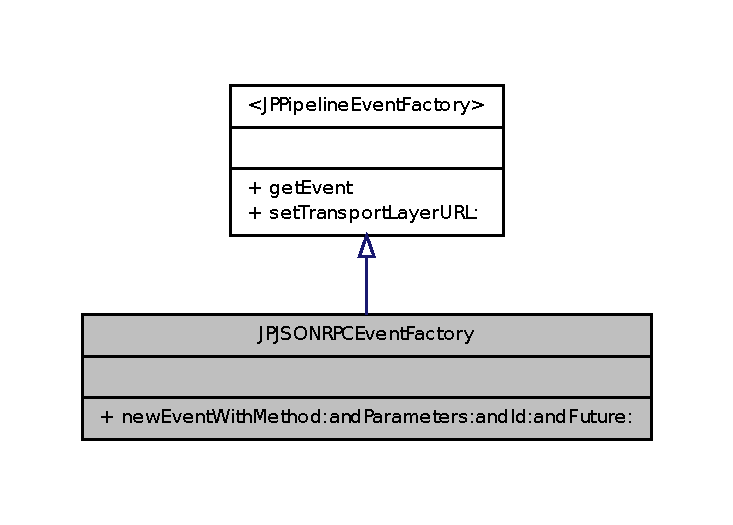
\includegraphics[width=352pt]{a00112}
\end{center}
\end{figure}


Collaboration diagram for JPJSONRPCEventFactory:\nopagebreak
\begin{figure}[H]
\begin{center}
\leavevmode
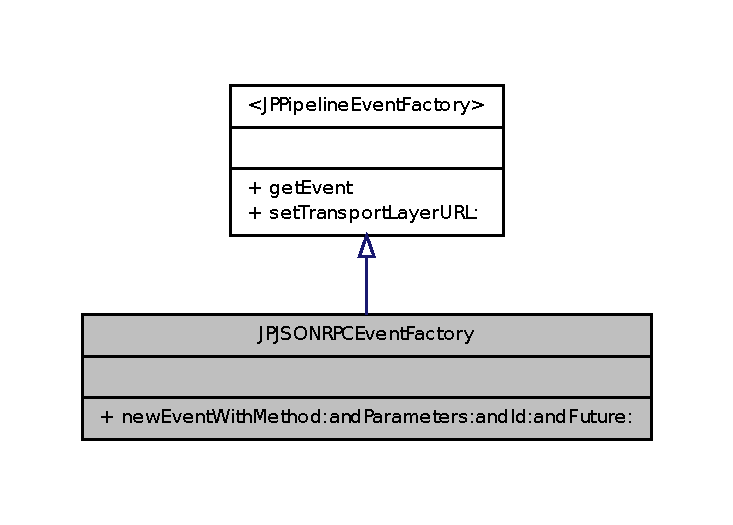
\includegraphics[width=352pt]{a00113}
\end{center}
\end{figure}
\subsection*{Static Public Member Functions}
\begin{DoxyCompactItemize}
\item 
(\hyperlink{a00018}{JPJSONRPCMessage} $\ast$) + \hyperlink{a00017_af9a34502ea4dfc99fa4a3c15d2323d7f}{newEventWithMethod:andParameters:andId:andFuture:}
\begin{DoxyCompactList}\small\item\em Build an \hyperlink{a00018}{JPJSONRPCMessage} event with this factory specifications. \item\end{DoxyCompactList}\end{DoxyCompactItemize}


\subsection{Detailed Description}
An protocol that represent \hyperlink{a00018}{JPJSONRPCMessage} factory pattern. 

\subsection{Member Function Documentation}
\hypertarget{a00017_af9a34502ea4dfc99fa4a3c15d2323d7f}{
\index{JPJSONRPCEventFactory@{JPJSONRPCEventFactory}!newEventWithMethod:andParameters:andId:andFuture:@{newEventWithMethod:andParameters:andId:andFuture:}}
\index{newEventWithMethod:andParameters:andId:andFuture:@{newEventWithMethod:andParameters:andId:andFuture:}!JPJSONRPCEventFactory@{JPJSONRPCEventFactory}}
\subsubsection[{newEventWithMethod:andParameters:andId:andFuture:}]{\setlength{\rightskip}{0pt plus 5cm}+ ({\bf JPJSONRPCMessage}$\ast$) newEventWithMethod: 
\begin{DoxyParamCaption}
\item[{dummy(NSString $\ast$)}]{anMethod}
\item[{andParameters:(NSArray $\ast$)}]{params}
\item[{andId:(NSNumber $\ast$)}]{anID}
\item[{andFuture:($<$ JPPipelineFuture $>$)}]{anFuture}
\end{DoxyParamCaption}
}}
\label{a00017_af9a34502ea4dfc99fa4a3c15d2323d7f}


Build an \hyperlink{a00018}{JPJSONRPCMessage} event with this factory specifications. 


\begin{DoxyParams}{Parameters}
{\em anMethod} & An RPC Method. \\
\hline
{\em params} & RPC Parameters. \\
\hline
{\em anID} & RPC Call id number. \\
\hline
{\em anFuture} & An \hyperlink{a00088}{JPPipelineFuture} object to get information about the progress of this event. \\
\hline
\end{DoxyParams}


The documentation for this class was generated from the following file:\begin{DoxyCompactItemize}
\item 
/Users/Paulo/Projects/JUMP/JUMPNetwork/Headers/JPJSONRPCEventFactory.h\end{DoxyCompactItemize}

\hypertarget{a00018}{
\section{JPJSONRPCMessage Class Reference}
\label{a00018}\index{JPJSONRPCMessage@{JPJSONRPCMessage}}
}


\hyperlink{a00018}{JPJSONRPCMessage} is an type of \hyperlink{a00006}{Event Message} that encapsulate an \href{http://en.wikipedia.org/wiki/JSON-RPC}{\tt JSON-\/RPC} data to be transported.  




{\ttfamily \#import $<$JPJSONRPCMessage.h$>$}



Inheritance diagram for JPJSONRPCMessage:
\nopagebreak
\begin{figure}[H]
\begin{center}
\leavevmode
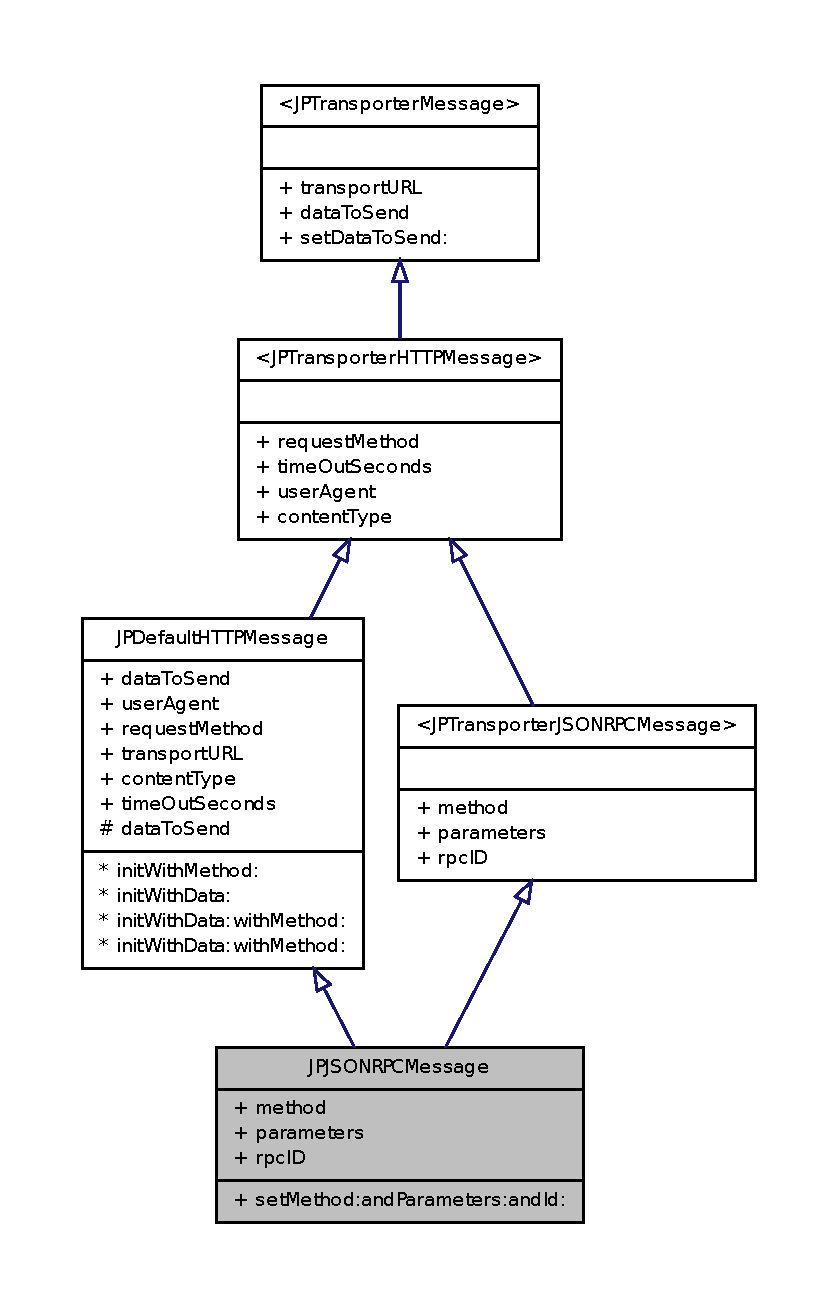
\includegraphics[height=600pt]{a00115}
\end{center}
\end{figure}


Collaboration diagram for JPJSONRPCMessage:
\nopagebreak
\begin{figure}[H]
\begin{center}
\leavevmode
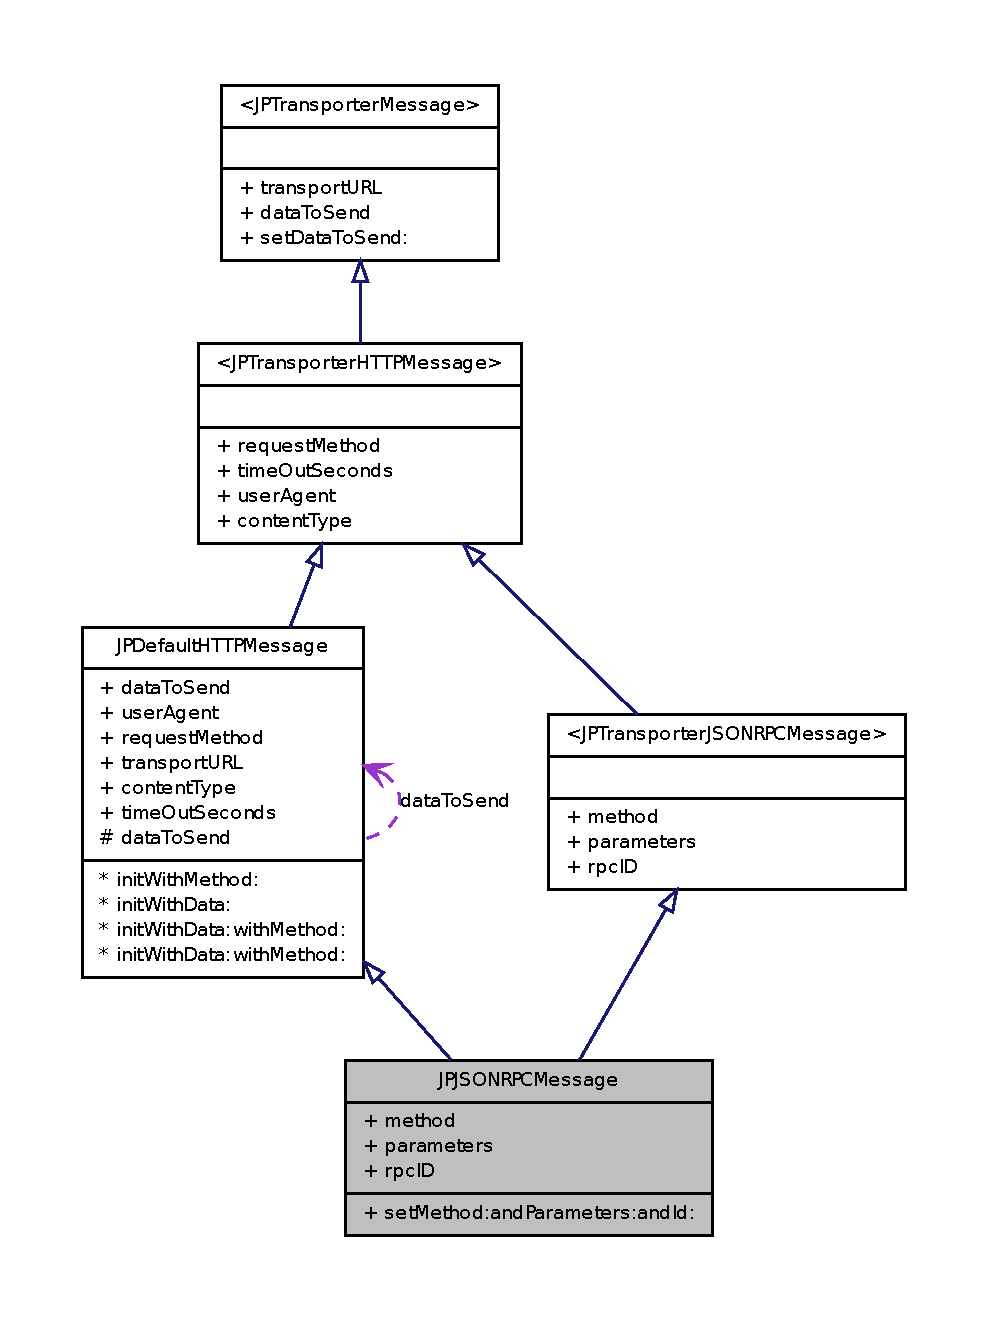
\includegraphics[width=400pt]{a00116}
\end{center}
\end{figure}
\subsection*{Public Member Functions}
\begin{DoxyCompactItemize}
\item 
(void) -\/ \hyperlink{a00018_ae4713c3b9ecb66103e48136775629b2b}{setMethod:andParameters:andId:}
\begin{DoxyCompactList}\small\item\em Configure the data of this event. \item\end{DoxyCompactList}\end{DoxyCompactItemize}
\subsection*{Properties}
\begin{DoxyCompactItemize}
\item 
\hypertarget{a00018_ae58ae13d4aad4b95c2a7cb5aa304bcc2}{
NSString $\ast$ \hyperlink{a00018_ae58ae13d4aad4b95c2a7cb5aa304bcc2}{method}}
\label{a00018_ae58ae13d4aad4b95c2a7cb5aa304bcc2}

\begin{DoxyCompactList}\small\item\em JSON-\/RPC Method. \item\end{DoxyCompactList}\item 
\hypertarget{a00018_a0da3510d87d44b6ead2d16aac67e6247}{
NSArray $\ast$ \hyperlink{a00018_a0da3510d87d44b6ead2d16aac67e6247}{parameters}}
\label{a00018_a0da3510d87d44b6ead2d16aac67e6247}

\begin{DoxyCompactList}\small\item\em JSON-\/RPC parameters. \item\end{DoxyCompactList}\item 
\hypertarget{a00018_afc35a8f75460f6d18f74cc5860b2df1b}{
NSNumber $\ast$ \hyperlink{a00018_afc35a8f75460f6d18f74cc5860b2df1b}{rpcID}}
\label{a00018_afc35a8f75460f6d18f74cc5860b2df1b}

\begin{DoxyCompactList}\small\item\em JSON-\/RPC id. \item\end{DoxyCompactList}\end{DoxyCompactItemize}


\subsection{Detailed Description}
\hyperlink{a00018}{JPJSONRPCMessage} is an type of \hyperlink{a00006}{Event Message} that encapsulate an \href{http://en.wikipedia.org/wiki/JSON-RPC}{\tt JSON-\/RPC} data to be transported. \hyperlink{a00018}{JPJSONRPCMessage} is an subclass of \hyperlink{a00012}{JPDefaultHTTPMessage} and implements the \hyperlink{a00041}{JPTransporterJSONRPCMessage} protocol, it is designed to transport \hyperlink{a00008}{JSON-\/RPC Event Messages} on top of the HTTP protocol. 

You can use this class directly, create your own subclass of this event or create your own implementation of the \hyperlink{a00041}{JPTransporterJSONRPCMessage} protocol. 

An simply code to illustrate how to send an \hyperlink{a00041}{JPTransporterJSONRPCMessage} downstream: 
\begin{DoxyCode}
 JPJSONRPCMessage *eventMessage = [JPJSONRPCMessage initWithMethod:@"POST"]
 eventMessage.transportURL = [NSURL URLWithString:@"http://seqoy.org/httpgateway"
      ];
 [eventMessage setMethod:@"someCall" 
           andParameters:[NSArray arrayWithObjects:@"parameter1", @"parameter2", 
      nil]
                   andId:[NSNumber numberWithInt:2]];
 
 [pipeline sendDownstream:[JPPipelineMessageEvent initWithMessage:eventMessage]];
      
\end{DoxyCode}
 Of course this example require a big boilerplate for a simple operation. See \hyperlink{a00004}{Using Factories} for more information to how configure and automate boilerplates using \href{http://en.wikipedia.org/wiki/Factory_method_pattern}{\tt Factory Patterns}. \par
 \par
 

\subsection{Member Function Documentation}
\hypertarget{a00018_ae4713c3b9ecb66103e48136775629b2b}{
\index{JPJSONRPCMessage@{JPJSONRPCMessage}!setMethod:andParameters:andId:@{setMethod:andParameters:andId:}}
\index{setMethod:andParameters:andId:@{setMethod:andParameters:andId:}!JPJSONRPCMessage@{JPJSONRPCMessage}}
\subsubsection[{setMethod:andParameters:andId:}]{\setlength{\rightskip}{0pt plus 5cm}-\/ (void) setMethod: 
\begin{DoxyParamCaption}
\item[{dummy(NSString $\ast$)}]{anMethod}
\item[{andParameters:(NSArray $\ast$)}]{params}
\item[{andId:(NSNumber $\ast$)}]{anID}
\end{DoxyParamCaption}
}}
\label{a00018_ae4713c3b9ecb66103e48136775629b2b}


Configure the data of this event. 


\begin{DoxyParams}{Parameters}
{\em anMethod} & An RPC method. \\
\hline
{\em params} & An array with parameters. \\
\hline
{\em anID} & ID of this RPC call. \\
\hline
\end{DoxyParams}


The documentation for this class was generated from the following file:\begin{DoxyCompactItemize}
\item 
/Users/Paulo/Projects/JUMP/JUMPNetwork/Headers/JPJSONRPCMessage.h\end{DoxyCompactItemize}

\hypertarget{a00019}{
\section{JPPipeline Class Reference}
\label{a00019}\index{JPPipeline@{JPPipeline}}
}


\hyperlink{a00019}{JPPipeline} is implementation of an presentation-\/tier request handling mechanism to receive many different types of requests.  




{\ttfamily \#import $<$JPPipeline.h$>$}



Collaboration diagram for JPPipeline:\nopagebreak
\begin{figure}[H]
\begin{center}
\leavevmode
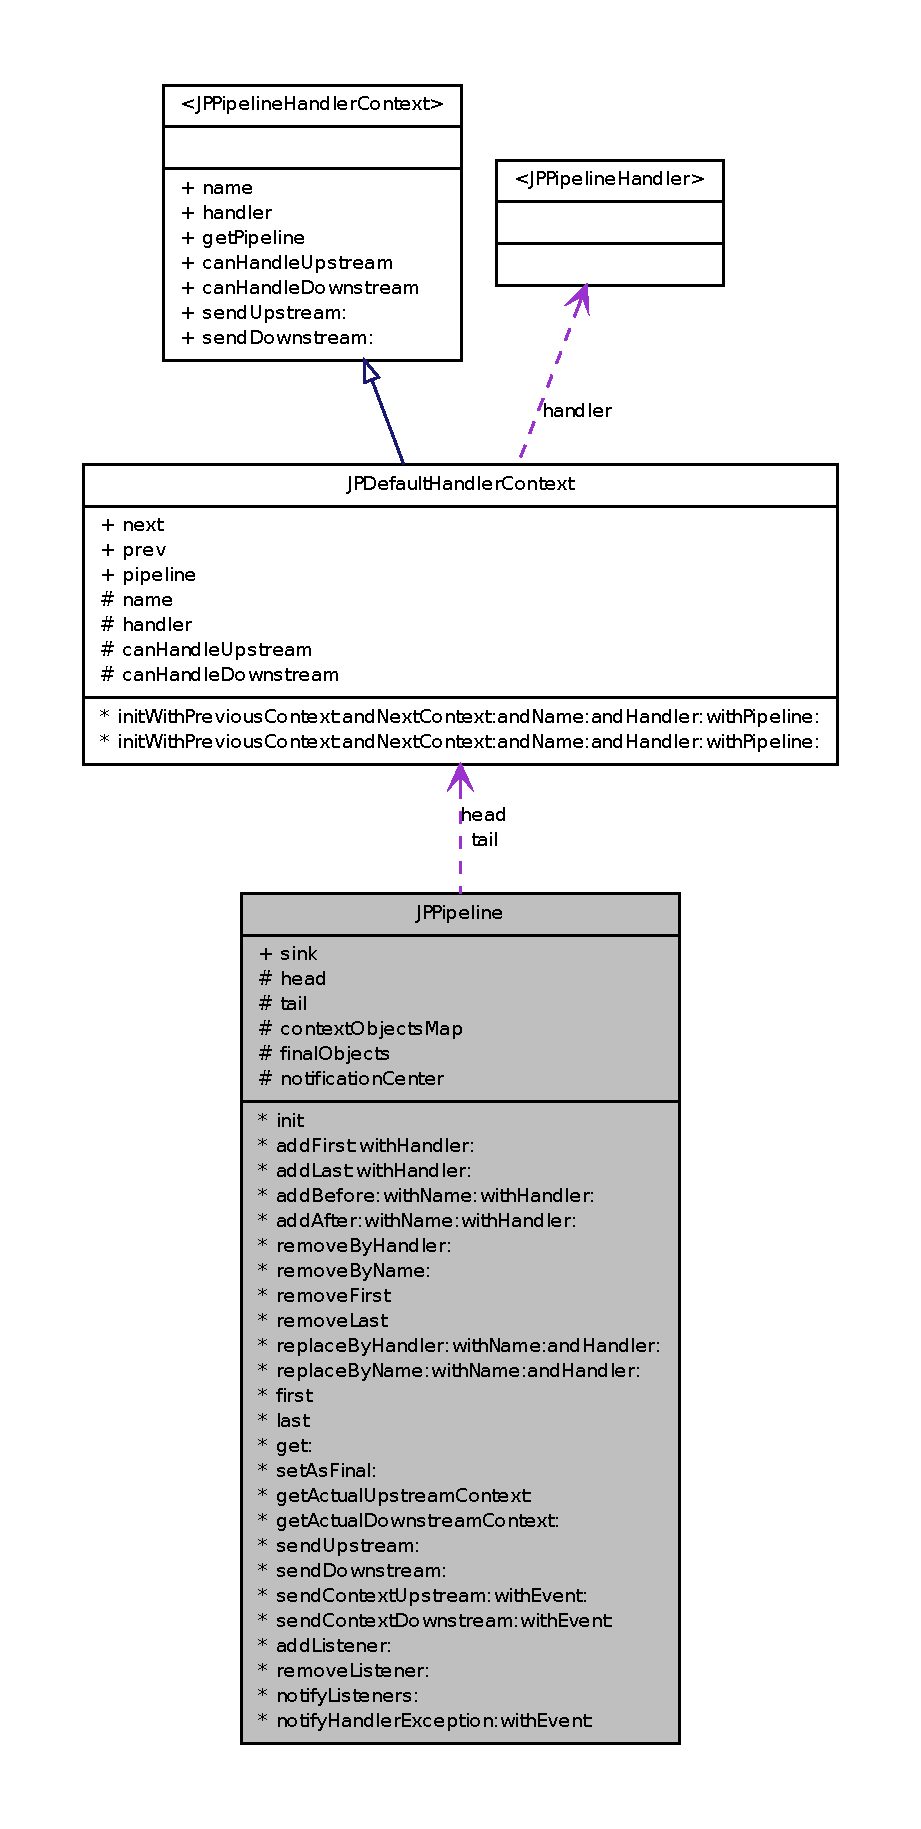
\includegraphics[height=600pt]{a00118}
\end{center}
\end{figure}
\subsection*{Properties}
\begin{DoxyCompactItemize}
\item 
$<$ \hyperlink{a00034}{JPPipelineSink} $>$ \hyperlink{a00019_a7bc8e0fa419b8dc01cf9e61ae59226ba}{sink}
\begin{DoxyCompactList}\small\item\em An \hyperlink{a00002}{I$|$O Transporter} implementation. \item\end{DoxyCompactList}\end{DoxyCompactItemize}
\subsection*{Init Methods}
\begin{DoxyCompactItemize}
\item 
\hypertarget{a00019_a848d7d1c1a53feff8ab706b5e1d06248}{
(id) + \hyperlink{a00019_a848d7d1c1a53feff8ab706b5e1d06248}{init}}
\label{a00019_a848d7d1c1a53feff8ab706b5e1d06248}

\begin{DoxyCompactList}\small\item\em Init the pipeline. \item\end{DoxyCompactList}\end{DoxyCompactItemize}
\subsection*{Add Handler Methods}
\begin{DoxyCompactItemize}
\item 
(void) -\/ \hyperlink{a00019_afe5f3b70a073f7e45d32ad6b0dcd4473}{addFirst:withHandler:}
\begin{DoxyCompactList}\small\item\em Inserts a Handler at the first position of this pipeline. \item\end{DoxyCompactList}\item 
(void) -\/ \hyperlink{a00019_a7a3cb65c4e376339b36fad298fb4674d}{addLast:withHandler:}
\begin{DoxyCompactList}\small\item\em Appends a Handler at the last position of this pipeline. \item\end{DoxyCompactList}\item 
(void) -\/ \hyperlink{a00019_a707e571dbe7a0d4011a32681d6c8b79d}{addBefore:withName:withHandler:}
\begin{DoxyCompactList}\small\item\em Inserts a \hyperlink{a00029}{JPPipelineHandler} before an existing handler of this pipeline. \item\end{DoxyCompactList}\item 
(void) -\/ \hyperlink{a00019_ace4814f6f5dc4e7cc0931af2a041eb7a}{addAfter:withName:withHandler:}
\begin{DoxyCompactList}\small\item\em Inserts a \hyperlink{a00029}{JPPipelineHandler} after an existing handler of this pipeline. \item\end{DoxyCompactList}\item 
\hypertarget{a00019_ac3feebdba37c2134e856e7a5ab02e434}{
(void) -\/ \hyperlink{a00019_ac3feebdba37c2134e856e7a5ab02e434}{removeByHandler:}}
\label{a00019_ac3feebdba37c2134e856e7a5ab02e434}

\begin{DoxyCompactList}\small\item\em Removes the specified \hyperlink{a00029}{JPPipelineHandler} from this pipeline. \item\end{DoxyCompactList}\item 
($<$ \hyperlink{a00029}{JPPipelineHandler} $>$) -\/ \hyperlink{a00019_aa7e27fa3a179bac1ab1aabaf779242b2}{removeByName:}
\begin{DoxyCompactList}\small\item\em Removes the \hyperlink{a00029}{JPPipelineHandler} with the specified name from this pipeline. \item\end{DoxyCompactList}\item 
($<$ \hyperlink{a00029}{JPPipelineHandler} $>$) -\/ \hyperlink{a00019_a81f7fa81d3aa6ad17e6129aa43ffe50e}{removeFirst}
\begin{DoxyCompactList}\small\item\em Removes the first \hyperlink{a00029}{JPPipelineHandler} in this pipeline. \item\end{DoxyCompactList}\item 
($<$ \hyperlink{a00029}{JPPipelineHandler} $>$) -\/ \hyperlink{a00019_a5d37aad9a88aa1da1505551c7c016e31}{removeLast}
\begin{DoxyCompactList}\small\item\em Removes the last \hyperlink{a00029}{JPPipelineHandler} in this pipeline. \item\end{DoxyCompactList}\end{DoxyCompactItemize}
\subsection*{Replace Handler Methods}
\begin{DoxyCompactItemize}
\item 
\hypertarget{a00019_a62c67fe5640ae0c53d564c945c77cde4}{
(void) -\/ \hyperlink{a00019_a62c67fe5640ae0c53d564c945c77cde4}{replaceByHandler:withName:andHandler:}}
\label{a00019_a62c67fe5640ae0c53d564c945c77cde4}

\begin{DoxyCompactList}\small\item\em Replaces the specified \hyperlink{a00029}{JPPipelineHandler} with a new handler in this pipeline. \item\end{DoxyCompactList}\item 
($<$ \hyperlink{a00029}{JPPipelineHandler} $>$) -\/ \hyperlink{a00019_a0030320bff9a07a4bda92076de0331e7}{replaceByName:withName:andHandler:}
\begin{DoxyCompactList}\small\item\em Replaces the \hyperlink{a00029}{JPPipelineHandler} of the specified name with a new handler in this pipeline. \item\end{DoxyCompactList}\end{DoxyCompactItemize}
\subsection*{Get Handler Methods}
\begin{DoxyCompactItemize}
\item 
($<$ \hyperlink{a00029}{JPPipelineHandler} $>$) -\/ \hyperlink{a00019_ab61ee133cd37d7b7ea31664a50f90beb}{first}
\begin{DoxyCompactList}\small\item\em Returns the first \hyperlink{a00029}{JPPipelineHandler} in this pipeline. \item\end{DoxyCompactList}\item 
($<$ \hyperlink{a00029}{JPPipelineHandler} $>$) -\/ \hyperlink{a00019_a8b3571a4e858f1b4a5ac659f5353a6ff}{last}
\begin{DoxyCompactList}\small\item\em Returns the last \hyperlink{a00029}{JPPipelineHandler} in this pipeline. \item\end{DoxyCompactList}\item 
($<$ \hyperlink{a00029}{JPPipelineHandler} $>$) -\/ \hyperlink{a00019_a08dc74fe2d73596ecda94f10ed3989f2}{get:}
\begin{DoxyCompactList}\small\item\em Returns the \hyperlink{a00029}{JPPipelineHandler} with the specified name in this pipeline. \item\end{DoxyCompactList}\item 
(void) -\/ \hyperlink{a00019_ad50160ab12c1c622a29d70fce1a58496}{setAsFinal:}
\begin{DoxyCompactList}\small\item\em Set handler as final, so he can't be removed or replaced. \item\end{DoxyCompactList}\item 
\hypertarget{a00019_a935af33ba729edcfe3781c6287ed3038}{
(\hyperlink{a00011}{JPDefaultHandlerContext} $\ast$) -\/ {\bfseries getActualUpstreamContext:}}
\label{a00019_a935af33ba729edcfe3781c6287ed3038}

\item 
\hypertarget{a00019_a02f42359af0eb3069c19768edd21731f}{
(\hyperlink{a00011}{JPDefaultHandlerContext} $\ast$) -\/ {\bfseries getActualDownstreamContext:}}
\label{a00019_a02f42359af0eb3069c19768edd21731f}

\end{DoxyCompactItemize}
\subsection*{Send Events Methods}
\begin{DoxyCompactItemize}
\item 
(void) -\/ \hyperlink{a00019_a2de87f8bb472f56d138e2862e88a5227}{sendUpstream:}
\begin{DoxyCompactList}\small\item\em Sends the specified \hyperlink{a00023}{JPPipelineEvent} to the first \hyperlink{a00035}{JPPipelineUpstreamHandler} in this pipeline. \item\end{DoxyCompactList}\item 
(void) -\/ \hyperlink{a00019_afa14dd597bfe8dee4e0621cd4e47a41c}{sendDownstream:}
\begin{DoxyCompactList}\small\item\em Sends the specified \hyperlink{a00023}{JPPipelineEvent} to the last \hyperlink{a00021}{JPPipelineDownstreamHandler} in this pipeline. \item\end{DoxyCompactList}\item 
\hypertarget{a00019_a120641c4888a9315350f2df2f1a93674}{
(void) -\/ {\bfseries sendContextUpstream:withEvent:}}
\label{a00019_a120641c4888a9315350f2df2f1a93674}

\item 
\hypertarget{a00019_a37d6a16b98ac9c7ab3d8d1b054ea2d17}{
(void) -\/ {\bfseries sendContextDownstream:withEvent:}}
\label{a00019_a37d6a16b98ac9c7ab3d8d1b054ea2d17}

\end{DoxyCompactItemize}
\subsection*{Listener Methods}
\begin{DoxyCompactItemize}
\item 
(void) -\/ \hyperlink{a00019_a80a40b033f9cb8c7f824c8dec2ef77d1}{addListener:}
\begin{DoxyCompactList}\small\item\em Adds one. \item\end{DoxyCompactList}\item 
(void) -\/ \hyperlink{a00019_a68ebd93ad1d12386be9c2a15cea7f02e}{removeListener:}
\begin{DoxyCompactList}\small\item\em Removes the specified listener. \item\end{DoxyCompactList}\item 
(void) -\/ \hyperlink{a00019_ae5febca680fe89e98ed28152a9d1f817}{notifyListeners:}
\begin{DoxyCompactList}\small\item\em Notify Some Action. \item\end{DoxyCompactList}\item 
(void) -\/ \hyperlink{a00019_a189266004e4fd48d0da86ed2f7ea5bc2}{notifyHandlerException:withEvent:}
\begin{DoxyCompactList}\small\item\em Send an \hyperlink{a00026}{JPPipelineException} when some exception is raised on a \hyperlink{a00023}{JPPipelineEvent}. \item\end{DoxyCompactList}\end{DoxyCompactItemize}


\subsection{Detailed Description}
\hyperlink{a00019}{JPPipeline} is implementation of an presentation-\/tier request handling mechanism to receive many different types of requests. \hyperlink{a00019}{JPPipeline} implements an advanced form of the \href{http://java.sun.com/blueprints/corej2eepatterns/Patterns/InterceptingFilter.html}{\tt Intercepting Filter Pattern} to give a user full control over how an event is handled and how the \hyperlink{a00029}{JPPipelineHandler} in the pipeline interact with each other.

\subsubsection*{How an event flows in a pipeline}

The following diagram describes how a \hyperlink{a00023}{Event} are processed by an \hyperlink{a00029}{Handler} in a \hyperlink{a00019}{Pipeline}. 

A \hyperlink{a00023}{JPPipelineEvent} can be handled by either a \hyperlink{a00035}{JPPipelineUpstreamHandler} or a \hyperlink{a00021}{JPPipelineDownstreamHandler} and be forwarded to the closest handler by calling \hyperlink{a00030_a9ab02ec0933865652634c54595ff7dd7}{sendUpstream: (JPPipelineHandlerContext-\/p)} or \hyperlink{a00030_a292ed51fe0b2e1ce6b2ed517be5fa5e8}{sendDownstream: (JPPipelineHandlerContext-\/p)}. The meaning of the event is interpreted somewhat differently depending on whether it is going upstream or going downstream. Please refer to \hyperlink{a00023}{JPPipelineEvent} for more information.



An upstream event is handled by the upstream handlers in the bottom-\/up direction as shown on the left side of the diagram. An upstream handler usually handles the inbound data on the bottom of the diagram. The inbound data is often read from a remote peer via the actual input operation. If an upstream event goes beyond the top upstream handler, it is discarded silently. 

A downstream event is handled by the downstream handler in the top-\/down direction as shown on the right side of the diagram. A downstream handler usually generates or transforms the outbound traffic such as write requests. If a downstream event goes beyond the bottom downstream handler, it is handled by an transporter object associated with the \hyperlink{a00019}{JPPipeline}. The transporter often performs the actual output operation. 

For example, let us assume that we created the following pipeline: 
\begin{DoxyCode}
 JPPipeline *p = [[JPPipeline init] retain];
 [p addLast:@"1" withHandler:[UpstreamHandlerA init]];
 [p addLast:@"2" withHandler:[UpstreamHandlerB init]];
 [p addLast:@"3" withHandler:[DownstreamHandlerA init]];
 [p addLast:@"4" withHandler:[DownstreamHandlerB init]];
 [p addLast:@"5" withHandler:[UpstreamHandlerX init]];
\end{DoxyCode}


In the example above, the class whose name starts with {\bfseries Upstream} means it is an upstream handler. The class whose name starts with {\bfseries Downstream} means it is a downstream handler. 

In the given example configuration, the handler evaluation order is 1, 2, 3, 4, 5 when an event goes upstream. When an event goes downstream, the order is 5, 4, 3, 2, 1. On top of this principle, \hyperlink{a00019}{JPPipeline} skips the evaluation of certain handlers to shorten the stack depth: 
\begin{DoxyItemize}
\item 3 and 4 don't implement \hyperlink{a00035}{JPPipelineUpstreamHandler}, and therefore the actual evaluation order of an upstream event will be: 1, 2, and 5. 
\item 1, 2, and 5 don't implement \hyperlink{a00021}{JPPipelineDownstreamHandler}, and therefore the actual evaluation order of a downstream event will be: 4 and 3. 
\item If 5 extended \hyperlink{a00038}{JPSimplePipelineHandler} which implements both \hyperlink{a00035}{JPPipelineUpstreamHandler} and \hyperlink{a00021}{JPPipelineDownstreamHandler}, the evaluation order of an upstream and a downstream event could be 1, 2, 5 and 5, 4, 3 respectively. 
\end{DoxyItemize}

\subsubsection*{Building a pipeline}

A user is supposed to have one or more \hyperlink{a00029}{JPPipelineHandler} in a pipeline to receive I/O events (e.g. read) and to request I/O operations (e.g. write). For example, a typical application will have the following handlers in each channel's pipeline, but your mileage may vary depending on the complexity and characteristics of the protocol and business logic:


\begin{DoxyEnumerate}
\item Protocol Decoder -\/ translates binary data into a Objective-\/C object. 
\item Protocol Encoder -\/ translates a Objective-\/C object into binary data. 
\item Business Logic Handler -\/ performs the actual business logic (e.g. database access). 
\end{DoxyEnumerate}

and it could be represented as shown in the following example:


\begin{DoxyCode}
 JPPipeline* pipeline = [[JPPipeline init] retain];
 [p addLast:@"decoder" withHandler:[MyProtocolDecoder init]];
 [p addLast:@"encoder" withHandler:[MyProtocolEncoder init]];
 [p addLast:@"handler" withHandler:[MyBusinessLogicHandler init]];
\end{DoxyCode}


\subsubsection*{Thread safety}

A \hyperlink{a00029}{JPPipelineHandler} can be added or removed at any time because a \hyperlink{a00019}{JPPipeline} is thread safe. For example, you can insert a {\bfseries SslHandler} when sensitive information is about to be exchanged, and remove it after the exchange.

\subsubsection*{Pitfall}

Due to the internal implementation detail of the current default \hyperlink{a00019}{JPPipeline}, the following code does not work as expected if {\ttfamily FirstHandler} is the last handler in the pipeline:


\begin{DoxyCode}
 @interface FirstHandler : JPSimplePipelineUpstreamHandler {}
 @end
 
 @implementation FirstHandler
 
 -(void)messageReceived:(<JPPipelineHandlerContext>)ctx withMessageEvent:(<
      JPPipelineMessageEvent>)e {
         // Remove this handler from the pipeline,
         [[ctx getPipeline] removeByHandler:self];
         // And let SecondHandler handle the current event.
         [[ctx getPipeline] addLast:@"2nd" withHandler:[SecondHandler init]];
         [ctx sendUpstream:e];
 }
 @end
\end{DoxyCode}


To implement the expected behavior, you have to add {\ttfamily SecondHandler} before the removal or make sure there is at least one more handler between {\ttfamily FirstHandler} and {\ttfamily SecondHandler}.  

\subsection{Member Function Documentation}
\hypertarget{a00019_afe5f3b70a073f7e45d32ad6b0dcd4473}{
\index{JPPipeline@{JPPipeline}!addFirst:withHandler:@{addFirst:withHandler:}}
\index{addFirst:withHandler:@{addFirst:withHandler:}!JPPipeline@{JPPipeline}}
\subsubsection[{addFirst:withHandler:}]{\setlength{\rightskip}{0pt plus 5cm}-\/ (void) addFirst: 
\begin{DoxyParamCaption}
\item[{dummy(NSString $\ast$)}]{name}
\item[{withHandler:($<$ {\bf JPPipelineHandler} $>$)}]{handler}
\end{DoxyParamCaption}
}}
\label{a00019_afe5f3b70a073f7e45d32ad6b0dcd4473}


Inserts a Handler at the first position of this pipeline. 


\begin{DoxyParams}{Parameters}
{\em name} & the name of the handler to insert first \\
\hline
{\em handler} & the handler to insert first \\
\hline
\end{DoxyParams}
\hypertarget{a00019_a7a3cb65c4e376339b36fad298fb4674d}{
\index{JPPipeline@{JPPipeline}!addLast:withHandler:@{addLast:withHandler:}}
\index{addLast:withHandler:@{addLast:withHandler:}!JPPipeline@{JPPipeline}}
\subsubsection[{addLast:withHandler:}]{\setlength{\rightskip}{0pt plus 5cm}-\/ (void) addLast: 
\begin{DoxyParamCaption}
\item[{dummy(NSString $\ast$)}]{name}
\item[{withHandler:($<$ {\bf JPPipelineHandler} $>$)}]{handler}
\end{DoxyParamCaption}
}}
\label{a00019_a7a3cb65c4e376339b36fad298fb4674d}


Appends a Handler at the last position of this pipeline. 


\begin{DoxyParams}{Parameters}
{\em name} & the name of the handler to append \\
\hline
{\em handler} & the handler to append \\
\hline
\end{DoxyParams}
\hypertarget{a00019_a707e571dbe7a0d4011a32681d6c8b79d}{
\index{JPPipeline@{JPPipeline}!addBefore:withName:withHandler:@{addBefore:withName:withHandler:}}
\index{addBefore:withName:withHandler:@{addBefore:withName:withHandler:}!JPPipeline@{JPPipeline}}
\subsubsection[{addBefore:withName:withHandler:}]{\setlength{\rightskip}{0pt plus 5cm}-\/ (void) addBefore: 
\begin{DoxyParamCaption}
\item[{dummy(NSString $\ast$)}]{baseName}
\item[{withName:(NSString $\ast$)}]{name}
\item[{withHandler:($<$ {\bf JPPipelineHandler} $>$)}]{handler}
\end{DoxyParamCaption}
}}
\label{a00019_a707e571dbe7a0d4011a32681d6c8b79d}


Inserts a \hyperlink{a00029}{JPPipelineHandler} before an existing handler of this pipeline. 


\begin{DoxyParams}{Parameters}
{\em baseName} & the name of the existing handler \\
\hline
{\em name} & the name of the handler to insert before \\
\hline
{\em handler} & the handler to insert before \\
\hline
\end{DoxyParams}
\hypertarget{a00019_ace4814f6f5dc4e7cc0931af2a041eb7a}{
\index{JPPipeline@{JPPipeline}!addAfter:withName:withHandler:@{addAfter:withName:withHandler:}}
\index{addAfter:withName:withHandler:@{addAfter:withName:withHandler:}!JPPipeline@{JPPipeline}}
\subsubsection[{addAfter:withName:withHandler:}]{\setlength{\rightskip}{0pt plus 5cm}-\/ (void) addAfter: 
\begin{DoxyParamCaption}
\item[{dummy(NSString $\ast$)}]{baseName}
\item[{withName:(NSString $\ast$)}]{name}
\item[{withHandler:($<$ {\bf JPPipelineHandler} $>$)}]{handler}
\end{DoxyParamCaption}
}}
\label{a00019_ace4814f6f5dc4e7cc0931af2a041eb7a}


Inserts a \hyperlink{a00029}{JPPipelineHandler} after an existing handler of this pipeline. 


\begin{DoxyParams}{Parameters}
{\em baseName} & the name of the existing handler \\
\hline
{\em name} & the name of the handler to insert after \\
\hline
{\em handler} & the handler to insert after \\
\hline
\end{DoxyParams}
\hypertarget{a00019_aa7e27fa3a179bac1ab1aabaf779242b2}{
\index{JPPipeline@{JPPipeline}!removeByName:@{removeByName:}}
\index{removeByName:@{removeByName:}!JPPipeline@{JPPipeline}}
\subsubsection[{removeByName:}]{\setlength{\rightskip}{0pt plus 5cm}-\/ ($<${\bf JPPipelineHandler}$>$) removeByName: 
\begin{DoxyParamCaption}
\item[{dummy(NSString $\ast$)}]{name}
\end{DoxyParamCaption}
}}
\label{a00019_aa7e27fa3a179bac1ab1aabaf779242b2}


Removes the \hyperlink{a00029}{JPPipelineHandler} with the specified name from this pipeline. 

\begin{DoxyReturn}{Returns}
the removed handler 
\end{DoxyReturn}
\hypertarget{a00019_a81f7fa81d3aa6ad17e6129aa43ffe50e}{
\index{JPPipeline@{JPPipeline}!removeFirst@{removeFirst}}
\index{removeFirst@{removeFirst}!JPPipeline@{JPPipeline}}
\subsubsection[{removeFirst}]{\setlength{\rightskip}{0pt plus 5cm}-\/ ($<${\bf JPPipelineHandler}$>$) removeFirst 
\begin{DoxyParamCaption}
{}
\end{DoxyParamCaption}
}}
\label{a00019_a81f7fa81d3aa6ad17e6129aa43ffe50e}


Removes the first \hyperlink{a00029}{JPPipelineHandler} in this pipeline. 

\begin{DoxyReturn}{Returns}
the removed handler 
\end{DoxyReturn}
\hypertarget{a00019_a5d37aad9a88aa1da1505551c7c016e31}{
\index{JPPipeline@{JPPipeline}!removeLast@{removeLast}}
\index{removeLast@{removeLast}!JPPipeline@{JPPipeline}}
\subsubsection[{removeLast}]{\setlength{\rightskip}{0pt plus 5cm}-\/ ($<${\bf JPPipelineHandler}$>$) removeLast 
\begin{DoxyParamCaption}
{}
\end{DoxyParamCaption}
}}
\label{a00019_a5d37aad9a88aa1da1505551c7c016e31}


Removes the last \hyperlink{a00029}{JPPipelineHandler} in this pipeline. 

\begin{DoxyReturn}{Returns}
the removed handler 
\end{DoxyReturn}
\hypertarget{a00019_a0030320bff9a07a4bda92076de0331e7}{
\index{JPPipeline@{JPPipeline}!replaceByName:withName:andHandler:@{replaceByName:withName:andHandler:}}
\index{replaceByName:withName:andHandler:@{replaceByName:withName:andHandler:}!JPPipeline@{JPPipeline}}
\subsubsection[{replaceByName:withName:andHandler:}]{\setlength{\rightskip}{0pt plus 5cm}-\/ ($<${\bf JPPipelineHandler}$>$) replaceByName: 
\begin{DoxyParamCaption}
\item[{dummy(NSString $\ast$)}]{oldName}
\item[{withName:(NSString $\ast$)}]{newName}
\item[{andHandler:($<$ {\bf JPPipelineHandler} $>$)}]{newHandler}
\end{DoxyParamCaption}
}}
\label{a00019_a0030320bff9a07a4bda92076de0331e7}


Replaces the \hyperlink{a00029}{JPPipelineHandler} of the specified name with a new handler in this pipeline. 

\begin{DoxyReturn}{Returns}
the removed handler 
\end{DoxyReturn}
\hypertarget{a00019_ab61ee133cd37d7b7ea31664a50f90beb}{
\index{JPPipeline@{JPPipeline}!first@{first}}
\index{first@{first}!JPPipeline@{JPPipeline}}
\subsubsection[{first}]{\setlength{\rightskip}{0pt plus 5cm}-\/ ($<${\bf JPPipelineHandler}$>$) first 
\begin{DoxyParamCaption}
{}
\end{DoxyParamCaption}
}}
\label{a00019_ab61ee133cd37d7b7ea31664a50f90beb}


Returns the first \hyperlink{a00029}{JPPipelineHandler} in this pipeline. 

\begin{DoxyReturn}{Returns}
the first handler or {\ttfamily nil} if this pipeline is empty. 
\end{DoxyReturn}
\hypertarget{a00019_a8b3571a4e858f1b4a5ac659f5353a6ff}{
\index{JPPipeline@{JPPipeline}!last@{last}}
\index{last@{last}!JPPipeline@{JPPipeline}}
\subsubsection[{last}]{\setlength{\rightskip}{0pt plus 5cm}-\/ ($<${\bf JPPipelineHandler}$>$) last 
\begin{DoxyParamCaption}
{}
\end{DoxyParamCaption}
}}
\label{a00019_a8b3571a4e858f1b4a5ac659f5353a6ff}


Returns the last \hyperlink{a00029}{JPPipelineHandler} in this pipeline. 

\begin{DoxyReturn}{Returns}
the last handler or {\ttfamily nil} if this pipeline is empty. 
\end{DoxyReturn}
\hypertarget{a00019_a08dc74fe2d73596ecda94f10ed3989f2}{
\index{JPPipeline@{JPPipeline}!get:@{get:}}
\index{get:@{get:}!JPPipeline@{JPPipeline}}
\subsubsection[{get:}]{\setlength{\rightskip}{0pt plus 5cm}-\/ ($<${\bf JPPipelineHandler}$>$) get: 
\begin{DoxyParamCaption}
\item[{dummy(NSString $\ast$)}]{name}
\end{DoxyParamCaption}
}}
\label{a00019_a08dc74fe2d73596ecda94f10ed3989f2}


Returns the \hyperlink{a00029}{JPPipelineHandler} with the specified name in this pipeline. 

\begin{DoxyReturn}{Returns}
the handler with the specified name or {\ttfamily nil} if there's no such handler in this pipeline. 
\end{DoxyReturn}
\hypertarget{a00019_ad50160ab12c1c622a29d70fce1a58496}{
\index{JPPipeline@{JPPipeline}!setAsFinal:@{setAsFinal:}}
\index{setAsFinal:@{setAsFinal:}!JPPipeline@{JPPipeline}}
\subsubsection[{setAsFinal:}]{\setlength{\rightskip}{0pt plus 5cm}-\/ (void) setAsFinal: 
\begin{DoxyParamCaption}
\item[{dummy(NSString $\ast$)}]{name}
\end{DoxyParamCaption}
}}
\label{a00019_ad50160ab12c1c622a29d70fce1a58496}


Set handler as final, so he can't be removed or replaced. 


\begin{DoxyParams}{Parameters}
{\em name} & the name of the handler to lock. \\
\hline
\end{DoxyParams}
\hypertarget{a00019_a2de87f8bb472f56d138e2862e88a5227}{
\index{JPPipeline@{JPPipeline}!sendUpstream:@{sendUpstream:}}
\index{sendUpstream:@{sendUpstream:}!JPPipeline@{JPPipeline}}
\subsubsection[{sendUpstream:}]{\setlength{\rightskip}{0pt plus 5cm}-\/ (void) sendUpstream: 
\begin{DoxyParamCaption}
\item[{dummy($<$ {\bf JPPipelineEvent} $>$)}]{e}
\end{DoxyParamCaption}
}}
\label{a00019_a2de87f8bb472f56d138e2862e88a5227}


Sends the specified \hyperlink{a00023}{JPPipelineEvent} to the first \hyperlink{a00035}{JPPipelineUpstreamHandler} in this pipeline. 


\begin{DoxyParams}{Parameters}
{\em e} & The \hyperlink{a00023}{JPPipelineEvent} to send upstream. \\
\hline
\end{DoxyParams}
\hypertarget{a00019_afa14dd597bfe8dee4e0621cd4e47a41c}{
\index{JPPipeline@{JPPipeline}!sendDownstream:@{sendDownstream:}}
\index{sendDownstream:@{sendDownstream:}!JPPipeline@{JPPipeline}}
\subsubsection[{sendDownstream:}]{\setlength{\rightskip}{0pt plus 5cm}-\/ (void) sendDownstream: 
\begin{DoxyParamCaption}
\item[{dummy($<$ {\bf JPPipelineEvent} $>$)}]{e}
\end{DoxyParamCaption}
}}
\label{a00019_afa14dd597bfe8dee4e0621cd4e47a41c}


Sends the specified \hyperlink{a00023}{JPPipelineEvent} to the last \hyperlink{a00021}{JPPipelineDownstreamHandler} in this pipeline. 


\begin{DoxyParams}{Parameters}
{\em e} & The \hyperlink{a00023}{JPPipelineEvent} to send downstream. \\
\hline
\end{DoxyParams}
\hypertarget{a00019_a80a40b033f9cb8c7f824c8dec2ef77d1}{
\index{JPPipeline@{JPPipeline}!addListener:@{addListener:}}
\index{addListener:@{addListener:}!JPPipeline@{JPPipeline}}
\subsubsection[{addListener:}]{\setlength{\rightskip}{0pt plus 5cm}-\/ (void) addListener: 
\begin{DoxyParamCaption}
\item[{dummy($<$ JPPipelineListener $>$)}]{listener}
\end{DoxyParamCaption}
}}
\label{a00019_a80a40b033f9cb8c7f824c8dec2ef77d1}


Adds one. 


\begin{DoxyParams}{Parameters}
{\em listener} & An \hyperlink{a00120}{JPPipelineListener} to get information about the pipeline operations. \\
\hline
\end{DoxyParams}
\hypertarget{a00019_a68ebd93ad1d12386be9c2a15cea7f02e}{
\index{JPPipeline@{JPPipeline}!removeListener:@{removeListener:}}
\index{removeListener:@{removeListener:}!JPPipeline@{JPPipeline}}
\subsubsection[{removeListener:}]{\setlength{\rightskip}{0pt plus 5cm}-\/ (void) removeListener: 
\begin{DoxyParamCaption}
\item[{dummy($<$ JPPipelineListener $>$)}]{listener}
\end{DoxyParamCaption}
}}
\label{a00019_a68ebd93ad1d12386be9c2a15cea7f02e}


Removes the specified listener. 


\begin{DoxyParams}{Parameters}
{\em listener} & An \hyperlink{a00120}{JPPipelineListener} to remove. \\
\hline
\end{DoxyParams}
\hypertarget{a00019_ae5febca680fe89e98ed28152a9d1f817}{
\index{JPPipeline@{JPPipeline}!notifyListeners:@{notifyListeners:}}
\index{notifyListeners:@{notifyListeners:}!JPPipeline@{JPPipeline}}
\subsubsection[{notifyListeners:}]{\setlength{\rightskip}{0pt plus 5cm}-\/ (void) notifyListeners: 
\begin{DoxyParamCaption}
\item[{dummy($<$ JPPipelineListenerNotification $>$)}]{notification}
\end{DoxyParamCaption}
}}
\label{a00019_ae5febca680fe89e98ed28152a9d1f817}


Notify Some Action. 


\begin{DoxyParams}{Parameters}
{\em notification} & An \hyperlink{a00121}{JPPipelineListenerNotification} to send to all listeners. \\
\hline
\end{DoxyParams}
\hypertarget{a00019_a189266004e4fd48d0da86ed2f7ea5bc2}{
\index{JPPipeline@{JPPipeline}!notifyHandlerException:withEvent:@{notifyHandlerException:withEvent:}}
\index{notifyHandlerException:withEvent:@{notifyHandlerException:withEvent:}!JPPipeline@{JPPipeline}}
\subsubsection[{notifyHandlerException:withEvent:}]{\setlength{\rightskip}{0pt plus 5cm}-\/ (void) notifyHandlerException: 
\begin{DoxyParamCaption}
\item[{dummy(NSException $\ast$)}]{exception}
\item[{withEvent:($<$ {\bf JPPipelineEvent} $>$)}]{e}
\end{DoxyParamCaption}
}}
\label{a00019_a189266004e4fd48d0da86ed2f7ea5bc2}


Send an \hyperlink{a00026}{JPPipelineException} when some exception is raised on a \hyperlink{a00023}{JPPipelineEvent}. 


\begin{DoxyParams}{Parameters}
{\em exception} & the {\ttfamily NSException} raised. \\
\hline
{\em e} & The \hyperlink{a00023}{JPPipelineEvent} that raise this exception. \\
\hline
\end{DoxyParams}


\subsection{Property Documentation}
\hypertarget{a00019_a7bc8e0fa419b8dc01cf9e61ae59226ba}{
\index{JPPipeline@{JPPipeline}!sink@{sink}}
\index{sink@{sink}!JPPipeline@{JPPipeline}}
\subsubsection[{sink}]{\setlength{\rightskip}{0pt plus 5cm}-\/ ($<$ {\bf JPPipelineSink} $>$) sink\hspace{0.3cm}{\ttfamily  \mbox{[}read, write, retain\mbox{]}}}}
\label{a00019_a7bc8e0fa419b8dc01cf9e61ae59226ba}


An \hyperlink{a00002}{I$|$O Transporter} implementation. 

\begin{DoxySeeAlso}{See also}
\hyperlink{a00034}{JPPipelineSink} and \hyperlink{a00002}{I$|$O Transporter} for more information. 
\end{DoxySeeAlso}


The documentation for this class was generated from the following file:\begin{DoxyCompactItemize}
\item 
/Users/Paulo/Projects/JUMP/JUMPNetwork/Headers/JPPipeline.h\end{DoxyCompactItemize}

\hypertarget{a00020}{
\section{JPPipelineDefaultFuture Class Reference}
\label{a00020}\index{JPPipelineDefaultFuture@{JPPipelineDefaultFuture}}
}


{\ttfamily \#import $<$JPPipelineDefaultFuture.h$>$}



Inherits JPPipelineFuture-\/p.



Collaboration diagram for JPPipelineDefaultFuture:\nopagebreak
\begin{figure}[H]
\begin{center}
\leavevmode
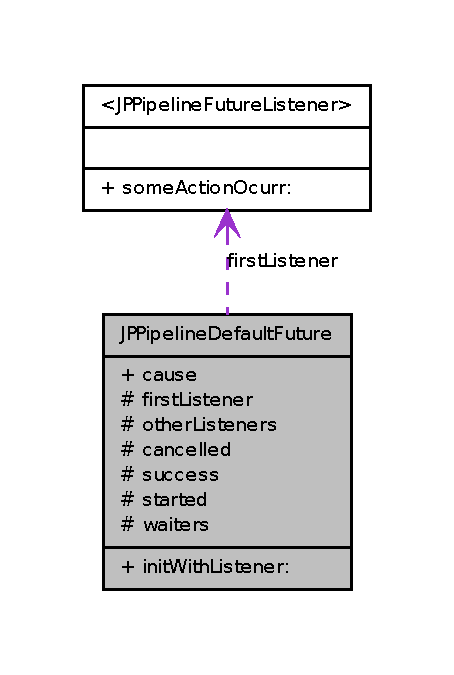
\includegraphics[width=218pt]{a00122}
\end{center}
\end{figure}


\subsection{Detailed Description}
/// /// ////// ////// ////// ////// ////// ////// ////// ////// ////// ////// ////// /// 

The documentation for this class was generated from the following file:\begin{DoxyCompactItemize}
\item 
/Users/Paulo/Projects/JUMP/JUMPNetwork/Headers/JPPipelineDefaultFuture.h\end{DoxyCompactItemize}

\hypertarget{a00021}{
\section{$<$JPPipelineDownstreamHandler$>$ Protocol Reference}
\label{a00021}\index{JPPipelineDownstreamHandler-\/p@{JPPipelineDownstreamHandler-\/p}}
}


Handles or intercepts a downstream \hyperlink{a00023}{JPPipelineEvent}, and sends a \hyperlink{a00023}{JPPipelineEvent} to the next handler in a \hyperlink{a00019}{JPPipeline}.  




{\ttfamily \#import $<$JPPipelineDownstreamHandler.h$>$}



Inheritance diagram for $<$JPPipelineDownstreamHandler$>$:\nopagebreak
\begin{figure}[H]
\begin{center}
\leavevmode
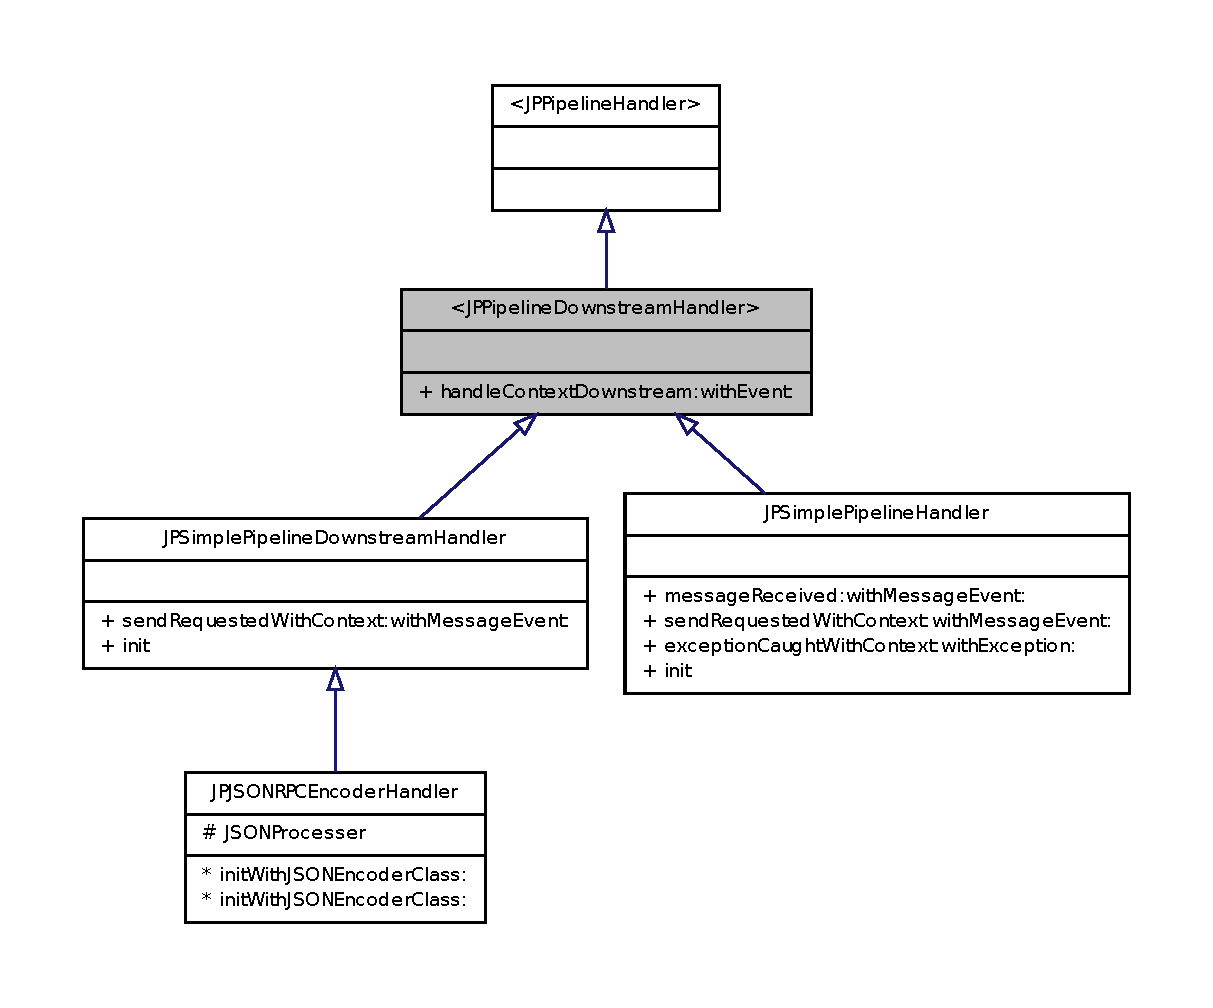
\includegraphics[width=400pt]{a00124}
\end{center}
\end{figure}


Collaboration diagram for $<$JPPipelineDownstreamHandler$>$:\nopagebreak
\begin{figure}[H]
\begin{center}
\leavevmode
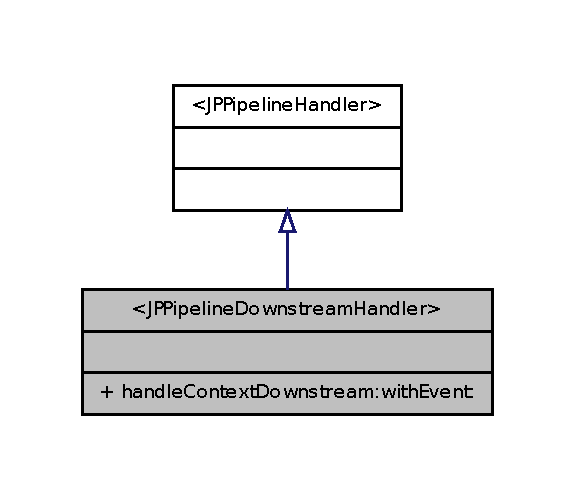
\includegraphics[width=276pt]{a00125}
\end{center}
\end{figure}
\subsection*{Public Member Functions}
\begin{DoxyCompactItemize}
\item 
(void) -\/ \hyperlink{a00021_a33230f19d46ee4dfd1d200767b00ddc9}{handleContextDownstream:withEvent:}
\begin{DoxyCompactList}\small\item\em Handles the specified downstream event. \item\end{DoxyCompactList}\end{DoxyCompactItemize}


\subsection{Detailed Description}
Handles or intercepts a downstream \hyperlink{a00023}{JPPipelineEvent}, and sends a \hyperlink{a00023}{JPPipelineEvent} to the next handler in a \hyperlink{a00019}{JPPipeline}. The most common use case of this interface is to intercept an request.

\subsubsection*{Using the Downstream Handler Class}

In most cases, you will get to use a \hyperlink{a00037}{JPSimplePipelineDownstreamHandler} to implement an upstream handler because it provides an individual handler method for each event type. You might want to implement this interface directly though if you want to handle various types of events in more generic way.

\paragraph*{Firing an event to the next handler}

You can forward the received event upstream or downstream. In most cases, \hyperlink{a00035}{JPPipelineUpstreamHandler} will send the event upstream (i.e. inbound) although it is legal to send the event downstream (i.e. outbound):


\begin{DoxyCode}
 // Sending the event upstream (inbound)
 -(void)handleContextDownstream:(JPDefaultHandlerContext*)ctx withEvent:(<
      JPPipelineEvent>)e {
         ...
         [ctx sendDownstream:e];
         ...
 }
 
 // Sending the event downstream (outbound)
 -(void)handleContextDownstream:(JPDefaultHandlerContext*)ctx withEvent:(<
      JPPipelineEvent>)e {
         ...
         [ctx sendUpstream:[UpstreamMessageEvent init(...)]];
         ...
 }
\end{DoxyCode}
 

\subsection{Member Function Documentation}
\hypertarget{a00021_a33230f19d46ee4dfd1d200767b00ddc9}{
\index{JPPipelineDownstreamHandler-\/p@{JPPipelineDownstreamHandler-\/p}!handleContextDownstream:withEvent:@{handleContextDownstream:withEvent:}}
\index{handleContextDownstream:withEvent:@{handleContextDownstream:withEvent:}!JPPipelineDownstreamHandler-p@{JPPipelineDownstreamHandler-\/p}}
\subsubsection[{handleContextDownstream:withEvent:}]{\setlength{\rightskip}{0pt plus 5cm}-\/ (void) handleContextDownstream: 
\begin{DoxyParamCaption}
\item[{dummy({\bf JPDefaultHandlerContext} $\ast$)}]{ctx}
\item[{withEvent:($<$ {\bf JPPipelineEvent} $>$)}]{e}
\end{DoxyParamCaption}
}}
\label{a00021_a33230f19d46ee4dfd1d200767b00ddc9}


Handles the specified downstream event. 


\begin{DoxyParams}{Parameters}
{\em ctx} & the context object for this handler \\
\hline
{\em e} & the downstream event to process or intercept \\
\hline
\end{DoxyParams}


The documentation for this protocol was generated from the following file:\begin{DoxyCompactItemize}
\item 
/Users/Paulo/Projects/JUMP/JUMPNetwork/Headers/JPPipelineDownstreamHandler.h\end{DoxyCompactItemize}

\hypertarget{a00022}{
\section{JPPipelineDowstreamMessageEvent Class Reference}
\label{a00022}\index{JPPipelineDowstreamMessageEvent@{JPPipelineDowstreamMessageEvent}}
}


The default dowstream Message Event implementation.  




{\ttfamily \#import $<$JPPipelineDowstreamMessageEvent.h$>$}



Inheritance diagram for JPPipelineDowstreamMessageEvent:\nopagebreak
\begin{figure}[H]
\begin{center}
\leavevmode
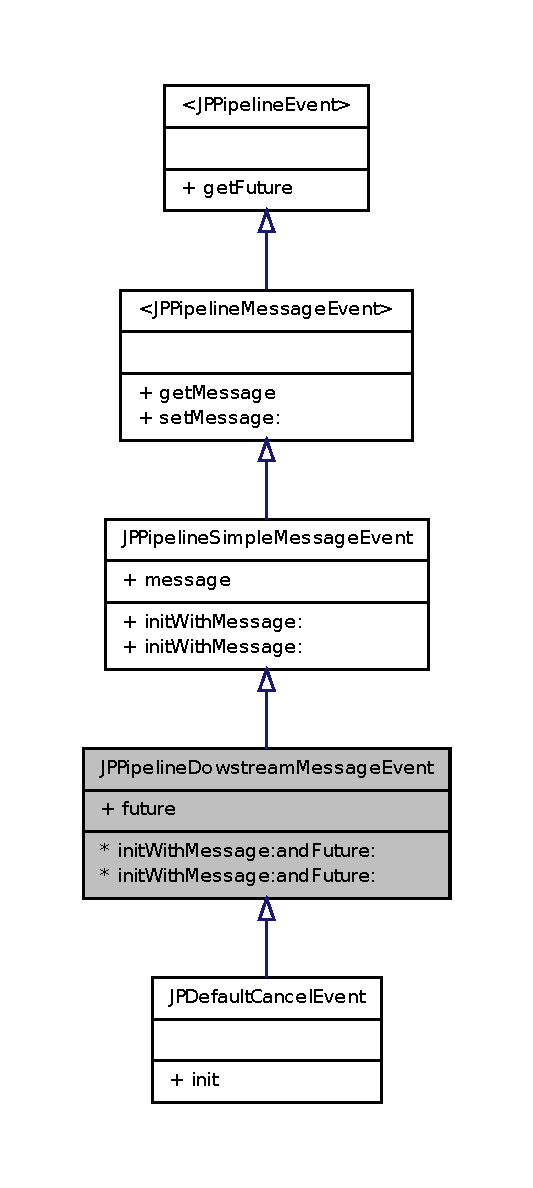
\includegraphics[width=256pt]{a00127}
\end{center}
\end{figure}


Collaboration diagram for JPPipelineDowstreamMessageEvent:\nopagebreak
\begin{figure}[H]
\begin{center}
\leavevmode
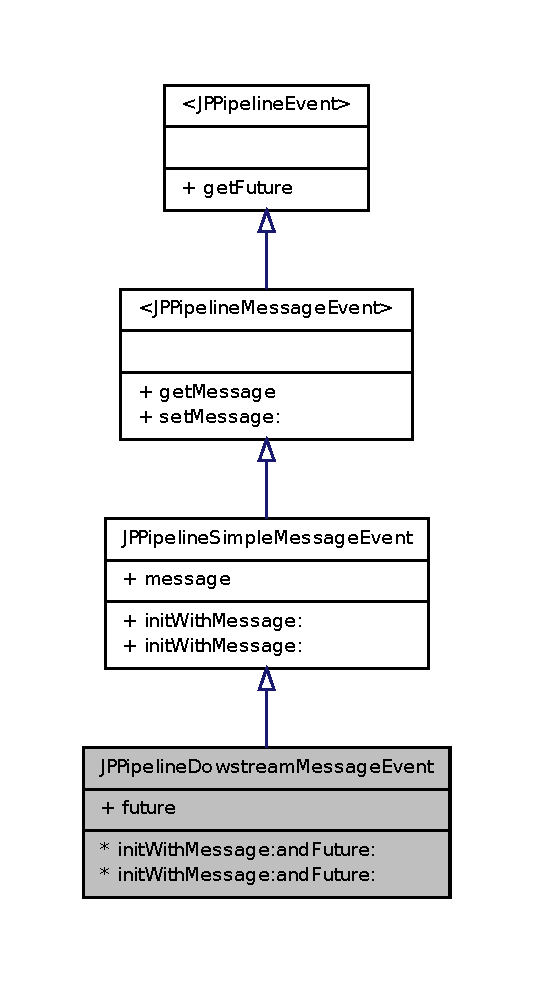
\includegraphics[width=256pt]{a00128}
\end{center}
\end{figure}
\subsection*{Properties}
\begin{DoxyCompactItemize}
\item 
\hypertarget{a00022_ab91b689523e7d730de35da0c2a892b8d}{
$<$ JPPipelineFuture $>$ \hyperlink{a00022_ab91b689523e7d730de35da0c2a892b8d}{future}}
\label{a00022_ab91b689523e7d730de35da0c2a892b8d}

\begin{DoxyCompactList}\small\item\em The \hyperlink{a00088}{JPPipelineFuture} object associated with this event. \item\end{DoxyCompactList}\end{DoxyCompactItemize}
\subsection*{Init Methods}
\begin{DoxyCompactItemize}
\item 
(id) + \hyperlink{a00022_adde91b7c2998797745d0a9235ecbb7a3}{initWithMessage:andFuture:}
\begin{DoxyCompactList}\small\item\em Init this event with the Message to transport and an Future to receive information about the progress. \item\end{DoxyCompactList}\item 
\hypertarget{a00022_adde91b7c2998797745d0a9235ecbb7a3}{
(id) -\/ {\bfseries initWithMessage:andFuture:}}
\label{a00022_adde91b7c2998797745d0a9235ecbb7a3}

\end{DoxyCompactItemize}


\subsection{Detailed Description}
The default dowstream Message Event implementation. 

\subsection{Member Function Documentation}
\hypertarget{a00022_adde91b7c2998797745d0a9235ecbb7a3}{
\index{JPPipelineDowstreamMessageEvent@{JPPipelineDowstreamMessageEvent}!initWithMessage:andFuture:@{initWithMessage:andFuture:}}
\index{initWithMessage:andFuture:@{initWithMessage:andFuture:}!JPPipelineDowstreamMessageEvent@{JPPipelineDowstreamMessageEvent}}
\subsubsection[{initWithMessage:andFuture:}]{\setlength{\rightskip}{0pt plus 5cm}+ (id) initWithMessage: 
\begin{DoxyParamCaption}
\item[{dummy(id)}]{anMessage}
\item[{andFuture:($<$ JPPipelineFuture $>$)}]{anListener}
\end{DoxyParamCaption}
}}
\label{a00022_adde91b7c2998797745d0a9235ecbb7a3}


Init this event with the Message to transport and an Future to receive information about the progress. 


\begin{DoxyParams}{Parameters}
{\em anMessage} & An object that represent the message. \\
\hline
{\em anListener} & An \hyperlink{a00088}{JPPipelineFuture} object to receive information about the progress. \\
\hline
\end{DoxyParams}


The documentation for this class was generated from the following file:\begin{DoxyCompactItemize}
\item 
/Users/Paulo/Projects/JUMP/JUMPNetwork/Headers/JPPipelineDowstreamMessageEvent.h\end{DoxyCompactItemize}

\hypertarget{a00023}{
\section{$<$JPPipelineEvent$>$ Protocol Reference}
\label{a00023}\index{JPPipelineEvent-\/p@{JPPipelineEvent-\/p}}
}


{\ttfamily \#import $<$JPPipelineEvent.h$>$}



Inheritance diagram for $<$JPPipelineEvent$>$:\nopagebreak
\begin{figure}[H]
\begin{center}
\leavevmode
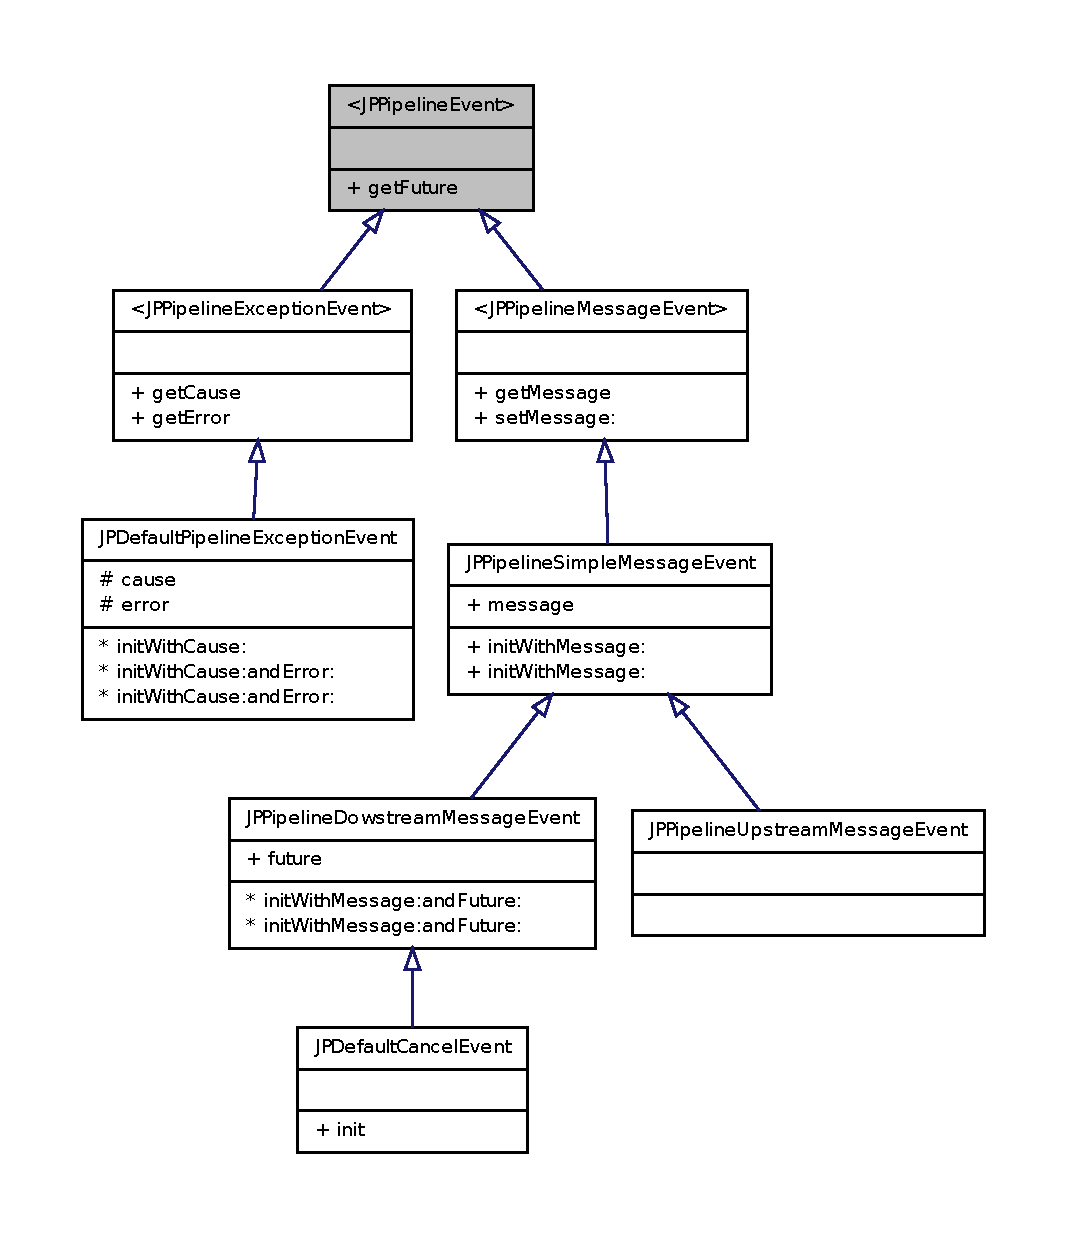
\includegraphics[width=400pt]{a00130}
\end{center}
\end{figure}
\subsection*{Public Member Functions}
\begin{DoxyCompactItemize}
\item 
($<$ JPPipelineFuture $>$) -\/ \hyperlink{a00023_a0b8f8fd9917015f408e32291719aa1ad}{getFuture}
\begin{DoxyCompactList}\small\item\em Returns the Future Object which is associated with this event. \item\end{DoxyCompactList}\end{DoxyCompactItemize}


\subsection{Detailed Description}
A \hyperlink{a00023}{JPPipelineEvent} is supposed to be handled by the \hyperlink{a00019}{JPPipeline} which is attached. Once an event is sent to a \hyperlink{a00019}{JPPipeline}, it is handled by a list of \hyperlink{a00029}{JPPipelineHandler}.

\subsubsection*{Upstream events and downstream events, and their interpretation}

Every event is either an upstream event or a downstream event. If an event flows forward from the first handler to the last handler in a \hyperlink{a00019}{JPPipeline}, we call it an upstream event and say {\bfseries \char`\"{}an
  event goes upstream.\char`\"{}} If an event flows backward from the last handler to the first handler in a \hyperlink{a00019}{JPPipeline}, we call it a downstream event and say {\bfseries \char`\"{}an event goes downstream.\char`\"{}} (Please refer to the diagram in \hyperlink{a00001}{The Pipeline} for more explanation.) 

When your server receives a \hyperlink{a00006}{message} from a client, the event associated with the received \hyperlink{a00006}{message} is an upstream event. When your server sends a \hyperlink{a00006}{message} or reply to the client, the event associated with the write request is a downstream event. The same rule applies for the client side. If your client sent a request to the server, it means your client triggered a downstream event. If your client received a response from the server, it means your client will be notified with an upstream event. Upstream events are often the result of inbound operations and downstream events are the request for outbound operations.

\subsubsection*{Cancelling Events}

You can {\bfseries cancel} an {\bfseries downstream} \hyperlink{a00005}{Event} while he is processing sending an \hyperlink{a00010}{JPDefaultCancelEvent} downstream as follow: 
\begin{DoxyCode}
 [pipeline sendDownstream:[JPDefaultCancelEvent init]];
\end{DoxyCode}
 \begin{DoxyNote}{Note}
Instead that \hyperlink{a00001}{The Pipeline} are always an asynchronous I/O operation he process one \hyperlink{a00005}{Event} at a time, that's why you can cancel an event while he is processing or waiting for some answer. 
\end{DoxyNote}


\subsubsection*{Default Events Messages Types}

\hyperlink{a00006}{Event Message} are some kind of data that is transported by an \hyperlink{a00005}{Event}. \hyperlink{a00006}{Event Message} doesn't have an defined type on the \hyperlink{a00001}{The Pipeline}. The {\bfseries type} of the \hyperlink{a00006}{Event Message} concern to the \hyperlink{a00003}{Handlers}. They use the {\bfseries Message Type} to known if they can handle or not. 

Also the \hyperlink{a00003}{Handlers} usually transform the message on his way through the \hyperlink{a00001}{The Pipeline}. 

{\bfseries JUMP Network} come with a bundled collection of \hyperlink{a00006}{Event Message} that you can use or reuse in your own subclasses.\par
 These are the main groups of this messages:
\begin{DoxyItemize}
\item \hyperlink{a00007}{HTTP Event Messages}
\item \hyperlink{a00008}{JSON-\/RPC Event Messages} 
\end{DoxyItemize}

\subsubsection*{Additional resources worth reading}

Please refer to the documentation of \hyperlink{a00029}{JPPipelineHandler} and its sub-\/types (\hyperlink{a00035}{JPPipelineUpstreamHandler} for upstream events and \hyperlink{a00021}{JPPipelineDownstreamHandler} for downstream events) to find out how a \hyperlink{a00023}{JPPipelineEvent} is interpreted depending on the type of the handler more in detail. Also, please refer to the \hyperlink{a00019}{JPPipeline} documentation to find out how an event flows in a pipeline. And \hyperlink{a00002}{I$|$O Transporter} to learn about I$|$O transporter and some default implementations.  

\subsection{Member Function Documentation}
\hypertarget{a00023_a0b8f8fd9917015f408e32291719aa1ad}{
\index{JPPipelineEvent-\/p@{JPPipelineEvent-\/p}!getFuture@{getFuture}}
\index{getFuture@{getFuture}!JPPipelineEvent-p@{JPPipelineEvent-\/p}}
\subsubsection[{getFuture}]{\setlength{\rightskip}{0pt plus 5cm}-\/ ($<$JPPipelineFuture$>$) getFuture 
\begin{DoxyParamCaption}
{}
\end{DoxyParamCaption}
}}
\label{a00023_a0b8f8fd9917015f408e32291719aa1ad}


Returns the Future Object which is associated with this event. 

If this event is an upstream event, this method will always return a SucceededPipelineFuture because the event has occurred already. If this event is a downstream event (i.e. I/O request), the returned future will be notified when the I/O request succeeds or fails. 

The documentation for this protocol was generated from the following file:\begin{DoxyCompactItemize}
\item 
/Users/Paulo/Projects/JUMP/JUMPNetwork/Headers/JPPipelineEvent.h\end{DoxyCompactItemize}

\hypertarget{a00024}{
\section{$<$JPPipelineEventFactory$>$ Protocol Reference}
\label{a00024}\index{JPPipelineEventFactory-\/p@{JPPipelineEventFactory-\/p}}
}


Creates a new Event.  




{\ttfamily \#import $<$JPPipelineEventFactory.h$>$}



Inheritance diagram for $<$JPPipelineEventFactory$>$:\nopagebreak
\begin{figure}[H]
\begin{center}
\leavevmode
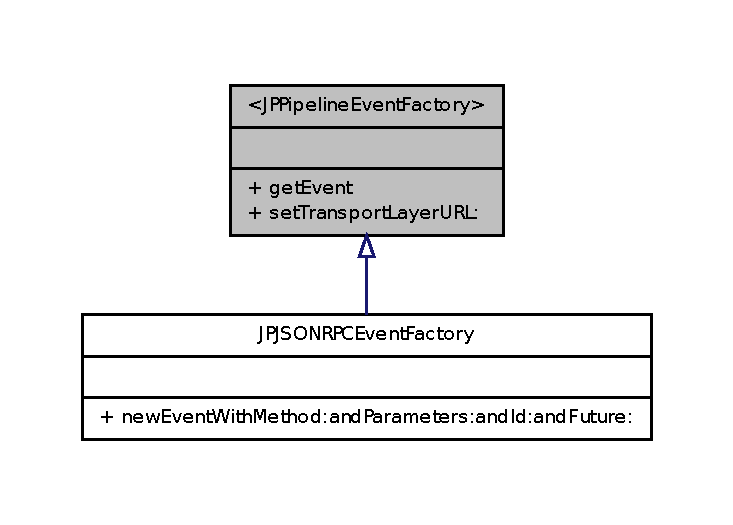
\includegraphics[width=352pt]{a00132}
\end{center}
\end{figure}
\subsection*{Static Public Member Functions}
\begin{DoxyCompactItemize}
\item 
\hypertarget{a00024_ad0137ddf845685a18b6c564de61f5037}{
($<$ \hyperlink{a00023}{JPPipelineEvent} $>$) + \hyperlink{a00024_ad0137ddf845685a18b6c564de61f5037}{getEvent}}
\label{a00024_ad0137ddf845685a18b6c564de61f5037}

\begin{DoxyCompactList}\small\item\em Returns a newly created Event. \item\end{DoxyCompactList}\item 
\hypertarget{a00024_a3ce6ec043e32712b94a7559f1a1aaf29}{
(void) + \hyperlink{a00024_a3ce6ec043e32712b94a7559f1a1aaf29}{setTransportLayerURL:}}
\label{a00024_a3ce6ec043e32712b94a7559f1a1aaf29}

\begin{DoxyCompactList}\small\item\em Set the Default Transport Layer URL. \item\end{DoxyCompactList}\end{DoxyCompactItemize}


\subsection{Detailed Description}
Creates a new Event. 

The documentation for this protocol was generated from the following file:\begin{DoxyCompactItemize}
\item 
/Users/Paulo/Projects/JUMP/JUMPNetwork/Headers/JPPipelineEventFactory.h\end{DoxyCompactItemize}

\hypertarget{a00025}{
\section{$<$JPPipelineEventListener$>$ Protocol Reference}
\label{a00025}\index{JPPipelineEventListener-\/p@{JPPipelineEventListener-\/p}}
}


A Event which represents the notification of an exception raised by a Handler.  




{\ttfamily \#import $<$JPPipelineEventListener.h$>$}

\subsection*{Public Member Functions}
\begin{DoxyCompactItemize}
\item 
\hypertarget{a00025_ab3f9aeae896ed993f51ecc1a9926bfc5}{
($<$ JPPipelineListener $>$) -\/ \hyperlink{a00025_ab3f9aeae896ed993f51ecc1a9926bfc5}{getListener}}
\label{a00025_ab3f9aeae896ed993f51ecc1a9926bfc5}

\begin{DoxyCompactList}\small\item\em Retrieve the Event Listener Object. \item\end{DoxyCompactList}\item 
\hypertarget{a00025_ad2a009d33860cbba56cbe01930191dda}{
(void) -\/ \hyperlink{a00025_ad2a009d33860cbba56cbe01930191dda}{setListener:}}
\label{a00025_ad2a009d33860cbba56cbe01930191dda}

\begin{DoxyCompactList}\small\item\em Set the Event Listener Object. \item\end{DoxyCompactList}\end{DoxyCompactItemize}


\subsection{Detailed Description}
A Event which represents the notification of an exception raised by a Handler. This event is for going upstream only. 

The documentation for this protocol was generated from the following file:\begin{DoxyCompactItemize}
\item 
/Users/Paulo/Projects/JUMP/JUMPNetwork/Headers/JPPipelineEventListener.h\end{DoxyCompactItemize}

\hypertarget{a00026}{
\section{JPPipelineException Class Reference}
\label{a00026}\index{JPPipelineException@{JPPipelineException}}
}


An subclass of {\ttfamily NSException} that represents an Generic Pipeline Exception.  




{\ttfamily \#import $<$JPPipelineException.h$>$}

\subsection*{Static Public Member Functions}
\begin{DoxyCompactItemize}
\item 
(id) + \hyperlink{a00026_a187f5aac71e8b126a9d362b88405ecbd}{initWithReason:}
\begin{DoxyCompactList}\small\item\em Init the exception. \item\end{DoxyCompactList}\end{DoxyCompactItemize}


\subsection{Detailed Description}
An subclass of {\ttfamily NSException} that represents an Generic Pipeline Exception. 

\subsection{Member Function Documentation}
\hypertarget{a00026_a187f5aac71e8b126a9d362b88405ecbd}{
\index{JPPipelineException@{JPPipelineException}!initWithReason:@{initWithReason:}}
\index{initWithReason:@{initWithReason:}!JPPipelineException@{JPPipelineException}}
\subsubsection[{initWithReason:}]{\setlength{\rightskip}{0pt plus 5cm}+ (id) initWithReason: 
\begin{DoxyParamCaption}
\item[{dummy(NSString $\ast$)}]{anReason}
\end{DoxyParamCaption}
}}
\label{a00026_a187f5aac71e8b126a9d362b88405ecbd}


Init the exception. 


\begin{DoxyParams}{Parameters}
{\em anReason} & The reason of this exception. \\
\hline
\end{DoxyParams}


The documentation for this class was generated from the following file:\begin{DoxyCompactItemize}
\item 
/Users/Paulo/Projects/JUMP/JUMPNetwork/Headers/JPPipelineException.h\end{DoxyCompactItemize}

\hypertarget{a00027}{
\section{$<$JPPipelineExceptionEvent$>$ Protocol Reference}
\label{a00027}\index{JPPipelineExceptionEvent-\/p@{JPPipelineExceptionEvent-\/p}}
}


A Event which represents the notification of an exception raised by a Handler.  




{\ttfamily \#import $<$JPPipelineExceptionEvent.h$>$}



Inheritance diagram for $<$JPPipelineExceptionEvent$>$:\nopagebreak
\begin{figure}[H]
\begin{center}
\leavevmode
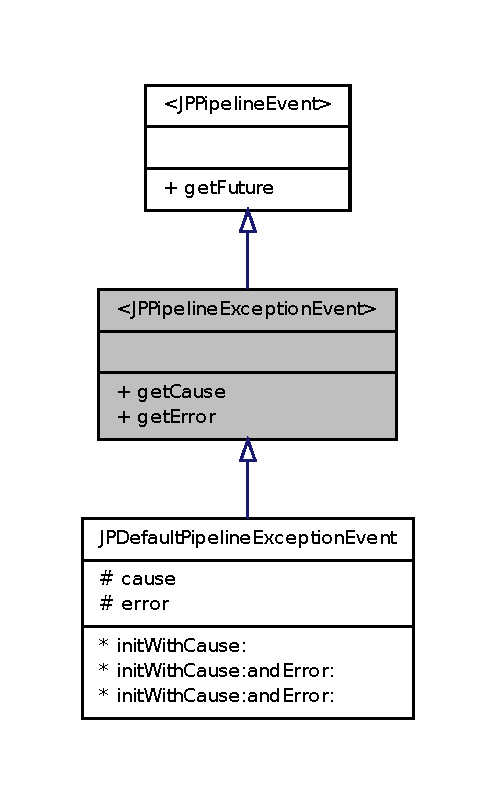
\includegraphics[width=238pt]{a00136}
\end{center}
\end{figure}


Collaboration diagram for $<$JPPipelineExceptionEvent$>$:\nopagebreak
\begin{figure}[H]
\begin{center}
\leavevmode
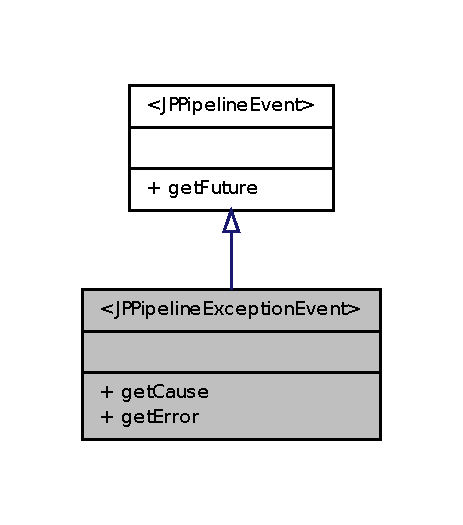
\includegraphics[width=222pt]{a00137}
\end{center}
\end{figure}
\subsection*{Public Member Functions}
\begin{DoxyCompactItemize}
\item 
\hypertarget{a00027_a98011afe1a6950c5aff925647fbd440a}{
(NSException $\ast$) -\/ \hyperlink{a00027_a98011afe1a6950c5aff925647fbd440a}{getCause}}
\label{a00027_a98011afe1a6950c5aff925647fbd440a}

\begin{DoxyCompactList}\small\item\em Returns the stored exception. \item\end{DoxyCompactList}\item 
\hypertarget{a00027_ae4f8fbaa0141878985c20bd477d777c8}{
(NSError $\ast$) -\/ \hyperlink{a00027_ae4f8fbaa0141878985c20bd477d777c8}{getError}}
\label{a00027_ae4f8fbaa0141878985c20bd477d777c8}

\begin{DoxyCompactList}\small\item\em Returns the stored error. \item\end{DoxyCompactList}\end{DoxyCompactItemize}


\subsection{Detailed Description}
A Event which represents the notification of an exception raised by a Handler. This event is for going upstream only. 

The documentation for this protocol was generated from the following file:\begin{DoxyCompactItemize}
\item 
/Users/Paulo/Projects/JUMP/JUMPNetwork/Headers/JPPipelineExceptionEvent.h\end{DoxyCompactItemize}

\hypertarget{a00028}{
\section{$<$JPPipelineFutureListener$>$ Protocol Reference}
\label{a00028}\index{JPPipelineFutureListener-\/p@{JPPipelineFutureListener-\/p}}
}


Listens to the result of a EventFuture.  




{\ttfamily \#import $<$JPPipelineFutureListener.h$>$}

\subsection*{Public Member Functions}
\begin{DoxyCompactItemize}
\item 
\hypertarget{a00028_a325c80e9415785f3737a6b992f2e8f1a}{
(void) -\/ \hyperlink{a00028_a325c80e9415785f3737a6b992f2e8f1a}{someActionOcurr:}}
\label{a00028_a325c80e9415785f3737a6b992f2e8f1a}

\begin{DoxyCompactList}\small\item\em Invoked when the I/O operation has been completed. \item\end{DoxyCompactList}\end{DoxyCompactItemize}


\subsection{Detailed Description}
Listens to the result of a EventFuture. The result of the asynchronous I/O operation is notified once this listener is added by calling addListener:. 

The documentation for this protocol was generated from the following file:\begin{DoxyCompactItemize}
\item 
/Users/Paulo/Projects/JUMP/JUMPNetwork/Headers/JPPipelineFutureListener.h\end{DoxyCompactItemize}

\hypertarget{a00029}{
\section{$<$JPPipelineHandler$>$ Protocol Reference}
\label{a00029}\index{JPPipelineHandler-\/p@{JPPipelineHandler-\/p}}
}


Handles or intercepts a Event, and sends a Event to the next handler in a Pipeline.  




{\ttfamily \#import $<$JPPipelineHandler.h$>$}



Inheritance diagram for $<$JPPipelineHandler$>$:\nopagebreak
\begin{figure}[H]
\begin{center}
\leavevmode
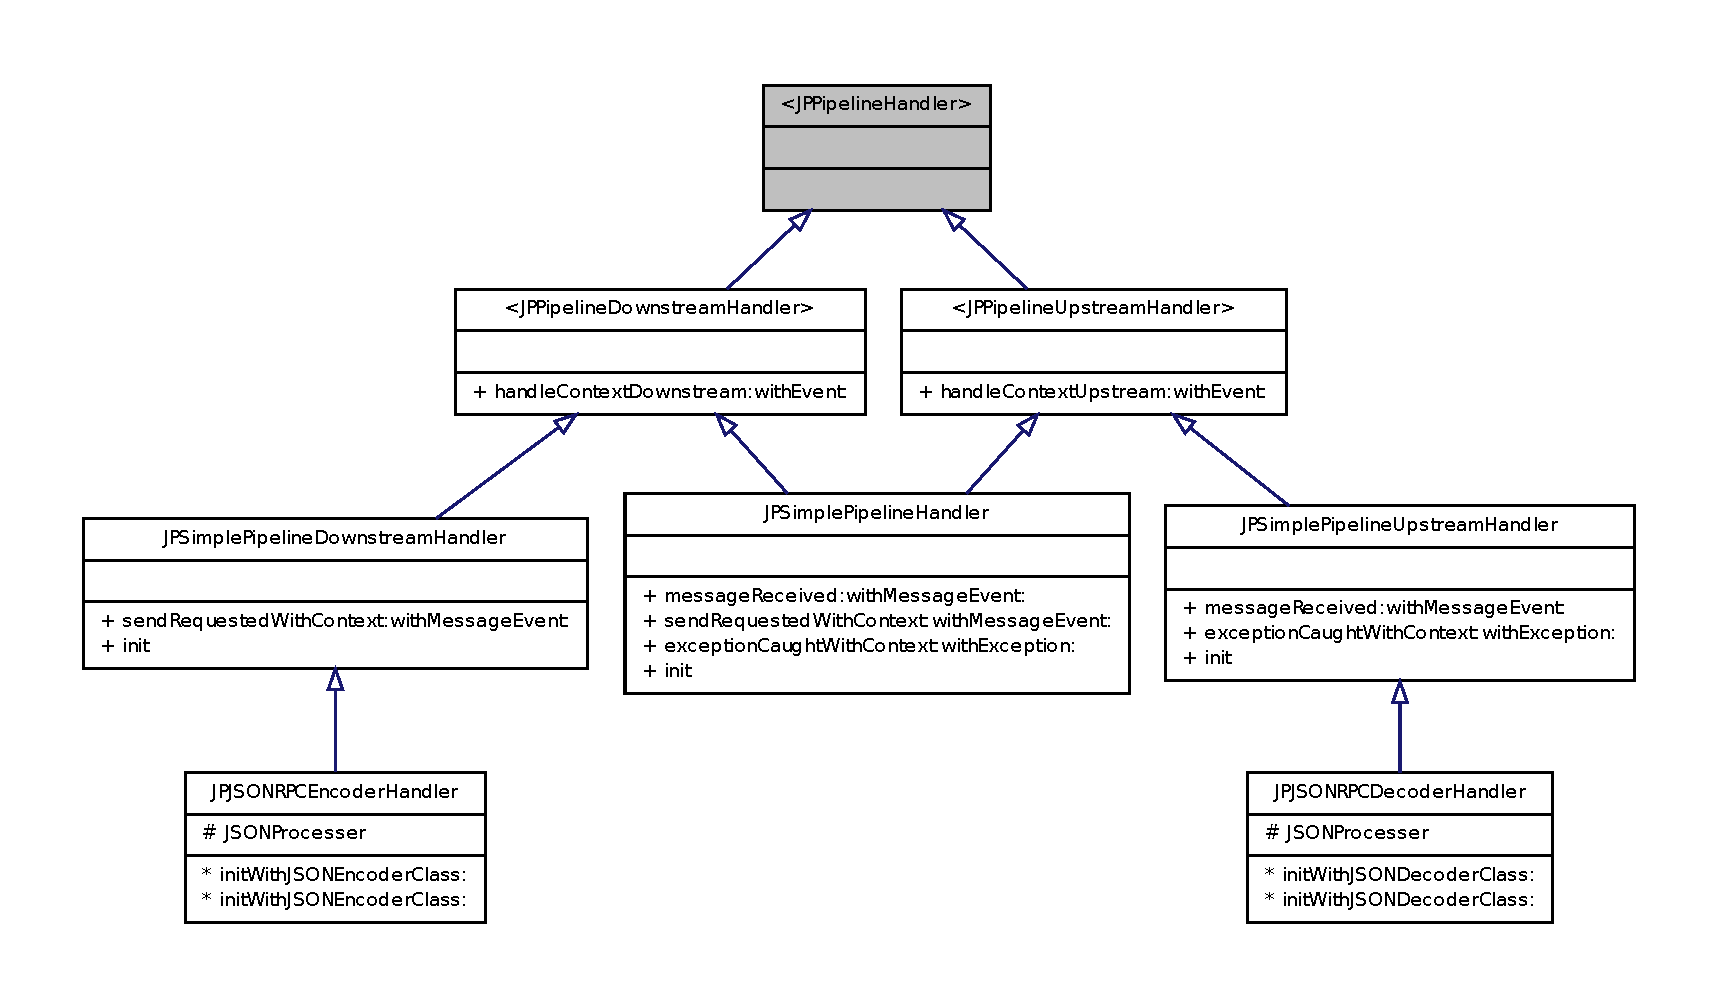
\includegraphics[width=400pt]{a00140}
\end{center}
\end{figure}


\subsection{Detailed Description}
Handles or intercepts a Event, and sends a Event to the next handler in a Pipeline. Pipeline Handler Protocol itself does not provide any method. To handle a Event you need to implement its sub-\/interfaces. There are two sub-\/interfaces which handles a received event, one for upstream events and the other for downstream events:


\begin{DoxyItemize}
\item \hyperlink{a00035}{JPPipelineUpstreamHandler} handles and intercepts an upstream Event.
\item \hyperlink{a00021}{JPPipelineDownstreamHandler} handles and intercepts a downstream Event.
\end{DoxyItemize}

You will also find more detailed explanation from the documentation of each sub-\/interface on how an event is interpreted when it goes upstream and downstream respectively.

\paragraph*{The context object}

A \hyperlink{a00029}{JPPipelineHandler} is provided with a \hyperlink{a00030}{JPPipelineHandlerContext} object. A \hyperlink{a00029}{JPPipelineHandler} is supposed to interact with the \hyperlink{a00019}{JPPipeline} it belongs to via a context object. Using the context object, the \hyperlink{a00029}{JPPipelineHandler} can pass events upstream or downstream, modify the pipeline dynamically, or store the information (attachment) which is specific to the handler. 

The documentation for this protocol was generated from the following file:\begin{DoxyCompactItemize}
\item 
/Users/Paulo/Projects/JUMP/JUMPNetwork/Headers/JPPipelineHandler.h\end{DoxyCompactItemize}

\hypertarget{a00030}{
\section{$<$JPPipelineHandlerContext$>$ Protocol Reference}
\label{a00030}\index{JPPipelineHandlerContext-\/p@{JPPipelineHandlerContext-\/p}}
}


Enables a \hyperlink{a00029}{JPPipelineHandler} to interact with its \hyperlink{a00019}{JPPipeline} and other handlers.  




{\ttfamily \#import $<$JPPipelineHandlerContext.h$>$}



Inheritance diagram for $<$JPPipelineHandlerContext$>$:\nopagebreak
\begin{figure}[H]
\begin{center}
\leavevmode
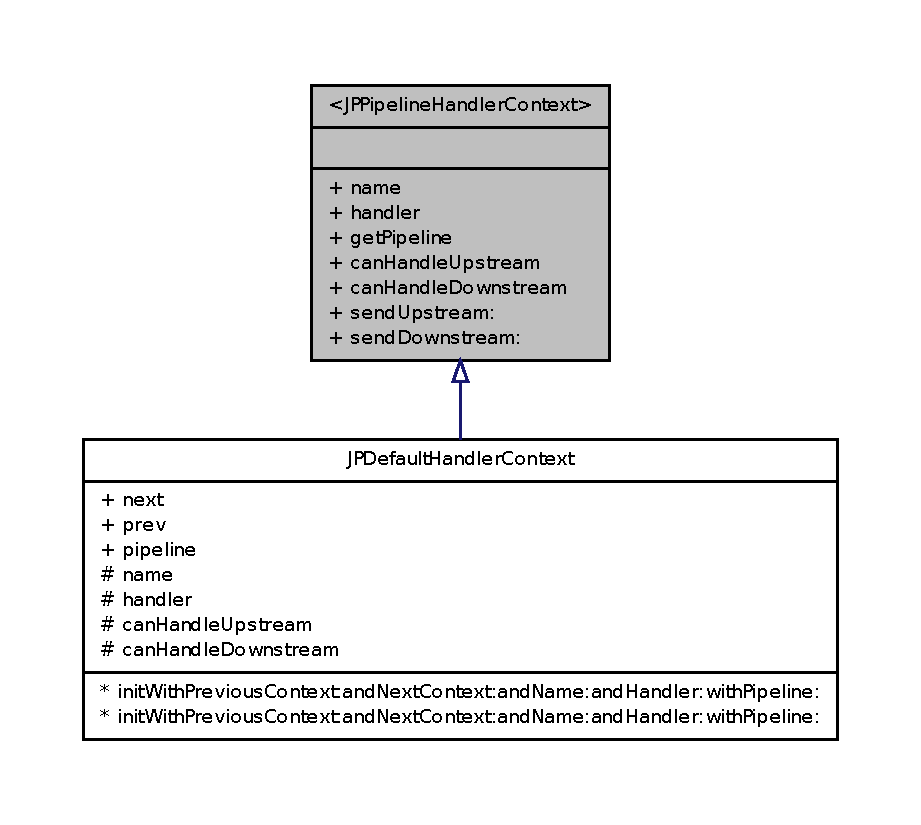
\includegraphics[width=400pt]{a00141}
\end{center}
\end{figure}
\subsection*{Public Member Functions}
\begin{DoxyCompactItemize}
\item 
\hypertarget{a00030_a8ac82545de840af4ed91e99ed6b8ecb2}{
(NSString $\ast$) -\/ \hyperlink{a00030_a8ac82545de840af4ed91e99ed6b8ecb2}{name}}
\label{a00030_a8ac82545de840af4ed91e99ed6b8ecb2}

\begin{DoxyCompactList}\small\item\em Returns the name of the \hyperlink{a00029}{JPPipelineHandler}. \item\end{DoxyCompactList}\item 
\hypertarget{a00030_a9cf37145f1fe22cbeb44c8848efc5d47}{
($<$ \hyperlink{a00029}{JPPipelineHandler} $>$) -\/ \hyperlink{a00030_a9cf37145f1fe22cbeb44c8848efc5d47}{handler}}
\label{a00030_a9cf37145f1fe22cbeb44c8848efc5d47}

\begin{DoxyCompactList}\small\item\em Returns the \hyperlink{a00029}{JPPipelineHandler} that this context object is serving. \item\end{DoxyCompactList}\item 
\hypertarget{a00030_a19bb45818df9ae3674732158f8d1cfd9}{
(\hyperlink{a00019}{JPPipeline} $\ast$) -\/ \hyperlink{a00030_a19bb45818df9ae3674732158f8d1cfd9}{getPipeline}}
\label{a00030_a19bb45818df9ae3674732158f8d1cfd9}

\begin{DoxyCompactList}\small\item\em Returns the Pipeline that this context belongs to. \item\end{DoxyCompactList}\item 
\hypertarget{a00030_a281202727bd690735f98851db6dd3d48}{
(BOOL) -\/ \hyperlink{a00030_a281202727bd690735f98851db6dd3d48}{canHandleUpstream}}
\label{a00030_a281202727bd690735f98851db6dd3d48}

\begin{DoxyCompactList}\small\item\em Returns YES if and only if the \hyperlink{a00029}{JPPipelineHandler} is an instance of \hyperlink{a00035}{JPPipelineUpstreamHandler}. \item\end{DoxyCompactList}\item 
\hypertarget{a00030_a4265a40ae2f3f6367a1fdfe7efe00fa6}{
(BOOL) -\/ \hyperlink{a00030_a4265a40ae2f3f6367a1fdfe7efe00fa6}{canHandleDownstream}}
\label{a00030_a4265a40ae2f3f6367a1fdfe7efe00fa6}

\begin{DoxyCompactList}\small\item\em Returns YES if and only if the \hyperlink{a00029}{JPPipelineHandler} is an instance of \hyperlink{a00021}{JPPipelineDownstreamHandler}. \item\end{DoxyCompactList}\item 
\hypertarget{a00030_a9ab02ec0933865652634c54595ff7dd7}{
(void) -\/ \hyperlink{a00030_a9ab02ec0933865652634c54595ff7dd7}{sendUpstream:}}
\label{a00030_a9ab02ec0933865652634c54595ff7dd7}

\begin{DoxyCompactList}\small\item\em Sends the specified \hyperlink{a00023}{JPPipelineEvent} to the \hyperlink{a00035}{JPPipelineUpstreamHandler} which is placed in the closest upstream from the handler associated with this context. \item\end{DoxyCompactList}\item 
\hypertarget{a00030_a292ed51fe0b2e1ce6b2ed517be5fa5e8}{
(void) -\/ \hyperlink{a00030_a292ed51fe0b2e1ce6b2ed517be5fa5e8}{sendDownstream:}}
\label{a00030_a292ed51fe0b2e1ce6b2ed517be5fa5e8}

\begin{DoxyCompactList}\small\item\em Sends the specified \hyperlink{a00023}{JPPipelineEvent} to the \hyperlink{a00021}{JPPipelineDownstreamHandler} which is placed in the closest downstream from the handler associated with this context. \item\end{DoxyCompactList}\end{DoxyCompactItemize}


\subsection{Detailed Description}
Enables a \hyperlink{a00029}{JPPipelineHandler} to interact with its \hyperlink{a00019}{JPPipeline} and other handlers. A handler can send a \hyperlink{a00023}{JPPipelineEvent} upstream or downstream, modify the \hyperlink{a00019}{JPPipeline} it belongs to dynamically.\par


\paragraph*{Sending an event}

You can send or forward a \hyperlink{a00023}{JPPipelineEvent} to the closest handler in the same \hyperlink{a00019}{JPPipeline} by calling sendUpstream(ChannelEvent) or sendDownstream(ChannelEvent). Please refer to \hyperlink{a00019}{JPPipeline} to understand how an event flows.

\paragraph*{Modifying a pipeline}

You can get the \hyperlink{a00019}{JPPipeline} your handler belongs to by calling \hyperlink{a00030_a19bb45818df9ae3674732158f8d1cfd9}{getPipeline (JPPipelineHandlerContext-\/p)}. A non-\/trivial application could insert, remove, or replace handlers in the pipeline dynamically in runtime.

\paragraph*{Retrieving for later use}

You can keep the \hyperlink{a00030}{JPPipelineHandlerContext} for later use, such as triggering an event outside the handler methods, even from a different thread.


\begin{DoxyCode}
 @interface MyHandler : JPSimplePipelineHandler {
        id<JPPipelineHandlerContext> savedCtx;
 }
 @end
 
 @implementation MyHandler
 
 -(void)beforeAdd:(<JPPipelineHandlerContextct>)ctx {
        savedCtx = ctx;
 }
 
 -(void)login:(NSString*)username andPassword:(NSString*)password {
        ... 
        [self login:username andPassword:password withSavedContext:savedCtx]; 
        ...
 }
 @end
\end{DoxyCode}


\paragraph*{Additional resources worth reading}

Please refer to the \hyperlink{a00029}{JPPipelineHandler}, \hyperlink{a00023}{JPPipelineEvent} and \hyperlink{a00019}{JPPipeline} to find out what a upstream event and a downstream event are, what fundamental differences they have, how they flow in a pipeline, and how to handle the event in your application. 

The documentation for this protocol was generated from the following file:\begin{DoxyCompactItemize}
\item 
/Users/Paulo/Projects/JUMP/JUMPNetwork/Headers/JPPipelineHandlerContext.h\end{DoxyCompactItemize}

\hypertarget{a00031}{
\section{$<$JPPipelineMessageEvent$>$ Protocol Reference}
\label{a00031}\index{JPPipelineMessageEvent-\/p@{JPPipelineMessageEvent-\/p}}
}


A \hyperlink{a00023}{JPPipelineEvent} which represents the transmission or reception of a \hyperlink{a00006}{message}.  




{\ttfamily \#import $<$JPPipelineMessageEvent.h$>$}



Inheritance diagram for $<$JPPipelineMessageEvent$>$:\nopagebreak
\begin{figure}[H]
\begin{center}
\leavevmode
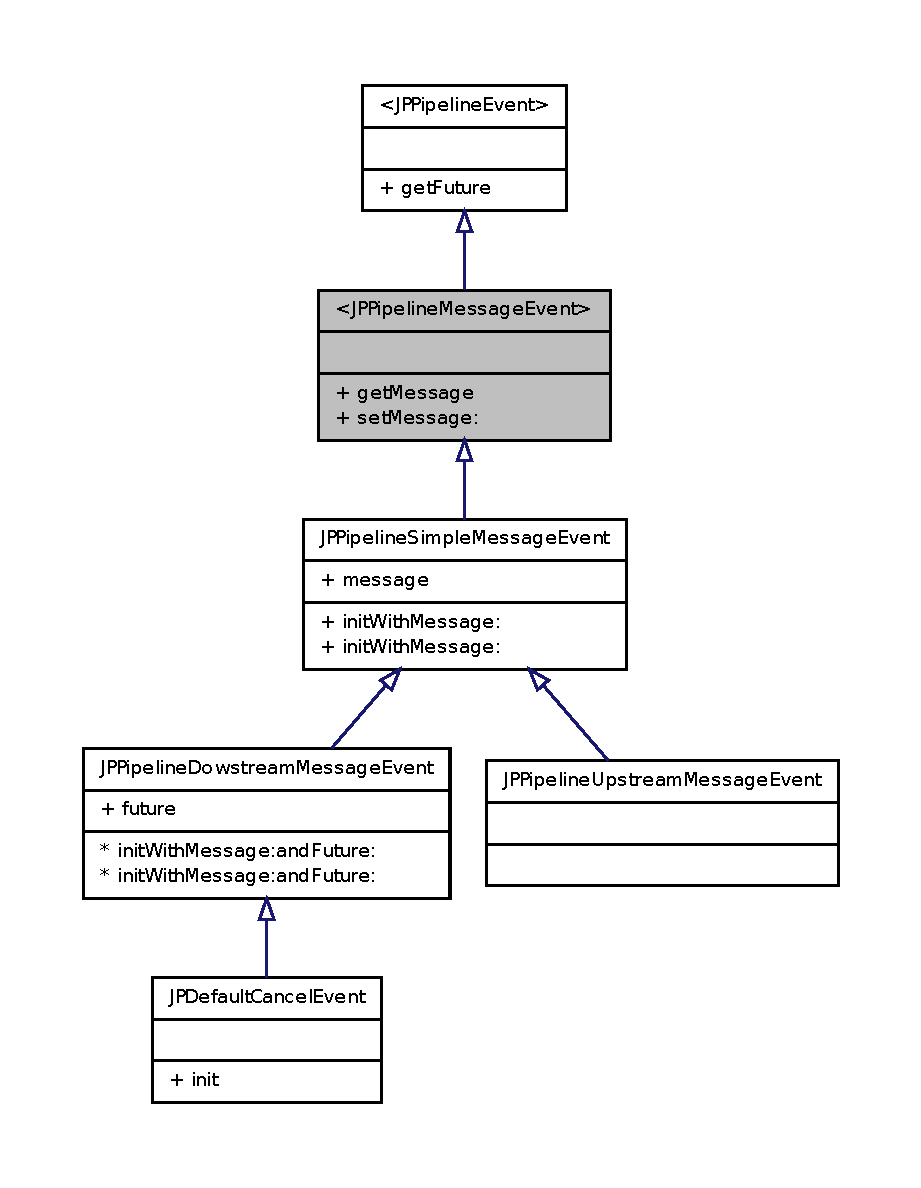
\includegraphics[width=400pt]{a00143}
\end{center}
\end{figure}


Collaboration diagram for $<$JPPipelineMessageEvent$>$:\nopagebreak
\begin{figure}[H]
\begin{center}
\leavevmode
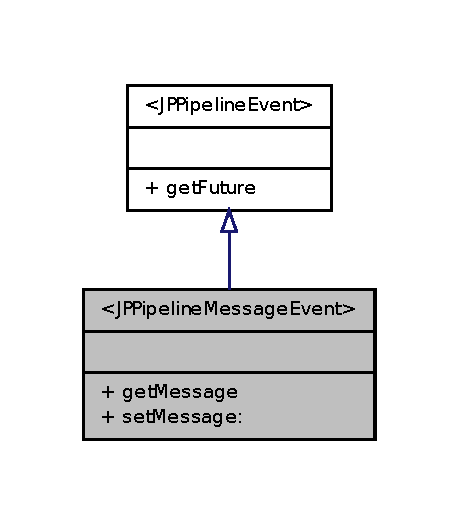
\includegraphics[width=220pt]{a00144}
\end{center}
\end{figure}
\subsection*{Public Member Functions}
\begin{DoxyCompactItemize}
\item 
\hypertarget{a00031_abbb8960b1919e3c10b28399e6836ed7a}{
(id) -\/ \hyperlink{a00031_abbb8960b1919e3c10b28399e6836ed7a}{getMessage}}
\label{a00031_abbb8960b1919e3c10b28399e6836ed7a}

\begin{DoxyCompactList}\small\item\em Returns the message. \item\end{DoxyCompactList}\item 
(void) -\/ \hyperlink{a00031_acf338a1e97066129630e13538ca904c3}{setMessage:}
\begin{DoxyCompactList}\small\item\em Set the message. \item\end{DoxyCompactList}\end{DoxyCompactItemize}


\subsection{Detailed Description}
A \hyperlink{a00023}{JPPipelineEvent} which represents the transmission or reception of a \hyperlink{a00006}{message}. It can mean the notification of a \hyperlink{a00006}{received message} or the request for sending a \hyperlink{a00006}{message}, depending on whether it is an upstream event or a downstream event respectively. Refer to the \hyperlink{a00023}{JPPipelineEvent} Protocol documentation to find out what an upstream event and a downstream event are and what fundamental differences they have. 

\subsection{Member Function Documentation}
\hypertarget{a00031_acf338a1e97066129630e13538ca904c3}{
\index{JPPipelineMessageEvent-\/p@{JPPipelineMessageEvent-\/p}!setMessage:@{setMessage:}}
\index{setMessage:@{setMessage:}!JPPipelineMessageEvent-p@{JPPipelineMessageEvent-\/p}}
\subsubsection[{setMessage:}]{\setlength{\rightskip}{0pt plus 5cm}-\/ (void) setMessage: 
\begin{DoxyParamCaption}
\item[{dummy(id)}]{anMessage}
\end{DoxyParamCaption}
\hspace{0.3cm}{\ttfamily  \mbox{[}required\mbox{]}}}}
\label{a00031_acf338a1e97066129630e13538ca904c3}


Set the message. 


\begin{DoxyParams}{Parameters}
{\em An} & \hyperlink{a00006}{Event Message} to be transported by this event. \\
\hline
\end{DoxyParams}


The documentation for this protocol was generated from the following file:\begin{DoxyCompactItemize}
\item 
/Users/Paulo/Projects/JUMP/JUMPNetwork/Headers/JPPipelineMessageEvent.h\end{DoxyCompactItemize}

\hypertarget{a00032}{
\section{JPPipelineNotification Class Reference}
\label{a00032}\index{JPPipelineNotification@{JPPipelineNotification}}
}


\hyperlink{a00032}{JPPipelineNotification} is an subclass of {\ttfamily NSNotification} that is used to receive information about the \hyperlink{a00019}{JPPipeline} operations.  




{\ttfamily \#import $<$JPPipelineNotification.h$>$}



Inherits JPPipelineListenerNotification-\/p.



\subsection{Detailed Description}
\hyperlink{a00032}{JPPipelineNotification} is an subclass of {\ttfamily NSNotification} that is used to receive information about the \hyperlink{a00019}{JPPipeline} operations. 

The documentation for this class was generated from the following file:\begin{DoxyCompactItemize}
\item 
/Users/Paulo/Projects/JUMP/JUMPNetwork/Headers/JPPipelineNotification.h\end{DoxyCompactItemize}

\hypertarget{a00033}{
\section{JPPipelineSimpleMessageEvent Class Reference}
\label{a00033}\index{JPPipelineSimpleMessageEvent@{JPPipelineSimpleMessageEvent}}
}


An {\bfseries Abstract Class} that define many methods to one Default Message Event implementation.  




{\ttfamily \#import $<$JPPipelineSimpleMessageEvent.h$>$}



Inheritance diagram for JPPipelineSimpleMessageEvent:\nopagebreak
\begin{figure}[H]
\begin{center}
\leavevmode
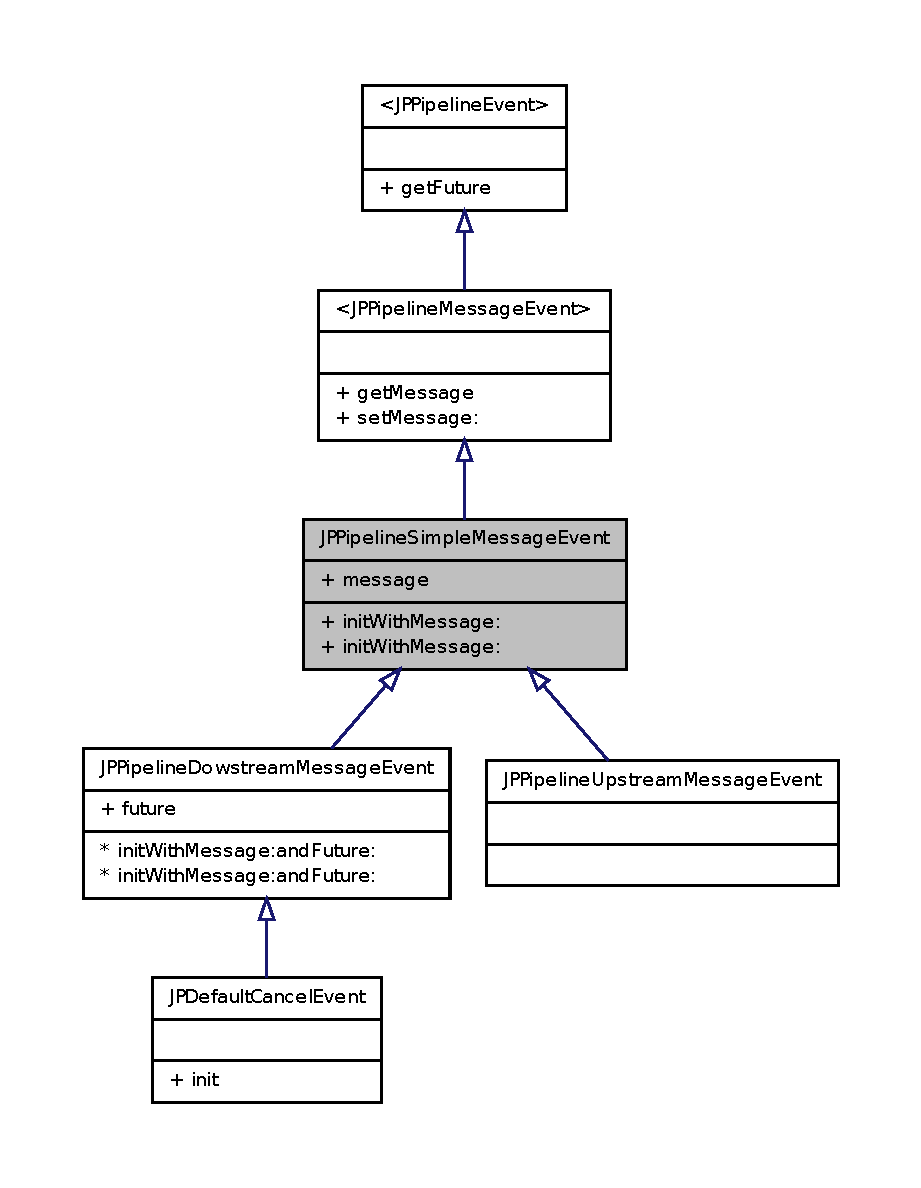
\includegraphics[width=400pt]{a00147}
\end{center}
\end{figure}


Collaboration diagram for JPPipelineSimpleMessageEvent:\nopagebreak
\begin{figure}[H]
\begin{center}
\leavevmode
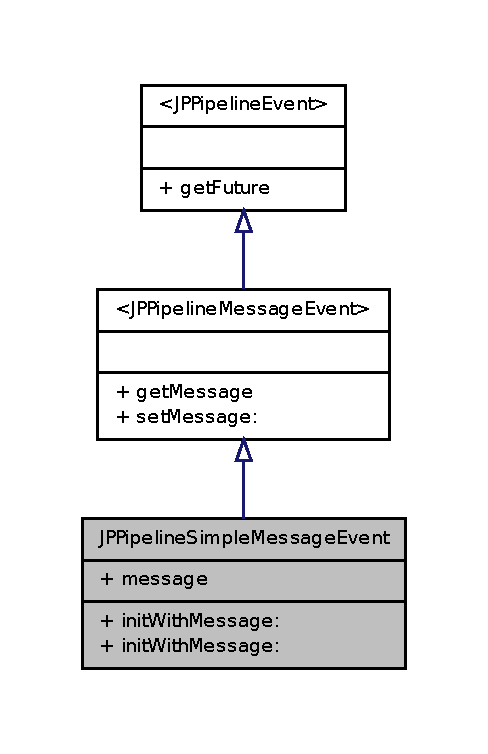
\includegraphics[width=234pt]{a00148}
\end{center}
\end{figure}
\subsection*{Static Public Member Functions}
\begin{DoxyCompactItemize}
\item 
(id) + \hyperlink{a00033_ae47d35264ae6b6465a2ec85bb6ac89f1}{initWithMessage:}
\begin{DoxyCompactList}\small\item\em Init this event with an message. \item\end{DoxyCompactList}\end{DoxyCompactItemize}
\subsection*{Properties}
\begin{DoxyCompactItemize}
\item 
\hypertarget{a00033_a13c199b5198314b666f2eea30d3900dc}{
id \hyperlink{a00033_a13c199b5198314b666f2eea30d3900dc}{message}}
\label{a00033_a13c199b5198314b666f2eea30d3900dc}

\begin{DoxyCompactList}\small\item\em The message associated with this event. \item\end{DoxyCompactList}\end{DoxyCompactItemize}


\subsection{Detailed Description}
An {\bfseries Abstract Class} that define many methods to one Default Message Event implementation. You should't initiate this class directly, one {\bfseries Exception} will be raised if you try so. You should subclass and implement some methods before use it. 

\subsection{Member Function Documentation}
\hypertarget{a00033_ae47d35264ae6b6465a2ec85bb6ac89f1}{
\index{JPPipelineSimpleMessageEvent@{JPPipelineSimpleMessageEvent}!initWithMessage:@{initWithMessage:}}
\index{initWithMessage:@{initWithMessage:}!JPPipelineSimpleMessageEvent@{JPPipelineSimpleMessageEvent}}
\subsubsection[{initWithMessage:}]{\setlength{\rightskip}{0pt plus 5cm}+ (id) initWithMessage: 
\begin{DoxyParamCaption}
\item[{dummy(id)}]{anMessage}
\end{DoxyParamCaption}
}}
\label{a00033_ae47d35264ae6b6465a2ec85bb6ac89f1}


Init this event with an message. 


\begin{DoxyParams}{Parameters}
{\em anMessage} & An message to associate with this event. \\
\hline
\end{DoxyParams}


The documentation for this class was generated from the following file:\begin{DoxyCompactItemize}
\item 
/Users/Paulo/Projects/JUMP/JUMPNetwork/Headers/JPPipelineSimpleMessageEvent.h\end{DoxyCompactItemize}

\hypertarget{a00034}{
\section{$<$JPPipelineSink$>$ Protocol Reference}
\label{a00034}\index{JPPipelineSink-\/p@{JPPipelineSink-\/p}}
}


Receives and processes the terminal downstream Event.  




{\ttfamily \#import $<$JPPipelineSink.h$>$}



Inheritance diagram for $<$JPPipelineSink$>$:\nopagebreak
\begin{figure}[H]
\begin{center}
\leavevmode
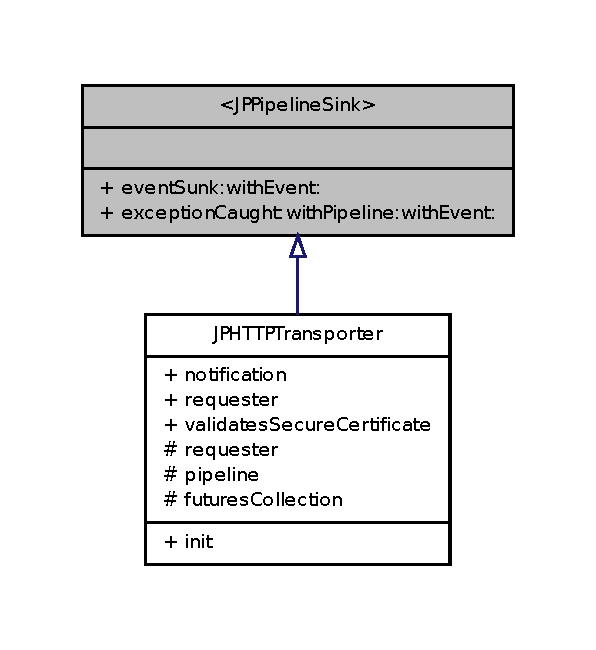
\includegraphics[width=286pt]{a00150}
\end{center}
\end{figure}
\subsection*{Public Member Functions}
\begin{DoxyCompactItemize}
\item 
(void) -\/ \hyperlink{a00034_a59e6e19fa75fbeff790d70d9aff76533}{eventSunk:withEvent:}
\begin{DoxyCompactList}\small\item\em Invoked by \hyperlink{a00019}{JPPipeline} when a downstream \hyperlink{a00023}{JPPipelineEvent} has reached its terminal (the head of the pipeline). \item\end{DoxyCompactList}\item 
(void) -\/ \hyperlink{a00034_af1cfabf45bca3d7b50af45c7c0d0323a}{exceptionCaught:withPipeline:withEvent:}
\begin{DoxyCompactList}\small\item\em Invoked by \hyperlink{a00019}{JPPipeline} when an exception was raised while one of its Handlers process a Event. \item\end{DoxyCompactList}\end{DoxyCompactItemize}


\subsection{Detailed Description}
Receives and processes the terminal downstream Event. A \hyperlink{a00034}{JPPipelineSink} is an internal component which is supposed to be implemented by a transport provider. See \hyperlink{a00002}{I$|$O Transporter} for more informations. 

\subsection{Member Function Documentation}
\hypertarget{a00034_a59e6e19fa75fbeff790d70d9aff76533}{
\index{JPPipelineSink-\/p@{JPPipelineSink-\/p}!eventSunk:withEvent:@{eventSunk:withEvent:}}
\index{eventSunk:withEvent:@{eventSunk:withEvent:}!JPPipelineSink-p@{JPPipelineSink-\/p}}
\subsubsection[{eventSunk:withEvent:}]{\setlength{\rightskip}{0pt plus 5cm}-\/ (void) eventSunk: 
\begin{DoxyParamCaption}
\item[{dummy({\bf JPPipeline} $\ast$)}]{pipeline}
\item[{withEvent:($<$ {\bf JPPipelineEvent} $>$)}]{e}
\end{DoxyParamCaption}
\hspace{0.3cm}{\ttfamily  \mbox{[}required\mbox{]}}}}
\label{a00034_a59e6e19fa75fbeff790d70d9aff76533}


Invoked by \hyperlink{a00019}{JPPipeline} when a downstream \hyperlink{a00023}{JPPipelineEvent} has reached its terminal (the head of the pipeline). 


\begin{DoxyParams}{Parameters}
{\em pipeline} & The pipeline that send the event. \\
\hline
{\em e} & The event. \\
\hline
\end{DoxyParams}
\hypertarget{a00034_af1cfabf45bca3d7b50af45c7c0d0323a}{
\index{JPPipelineSink-\/p@{JPPipelineSink-\/p}!exceptionCaught:withPipeline:withEvent:@{exceptionCaught:withPipeline:withEvent:}}
\index{exceptionCaught:withPipeline:withEvent:@{exceptionCaught:withPipeline:withEvent:}!JPPipelineSink-p@{JPPipelineSink-\/p}}
\subsubsection[{exceptionCaught:withPipeline:withEvent:}]{\setlength{\rightskip}{0pt plus 5cm}-\/ (void) exceptionCaught: 
\begin{DoxyParamCaption}
\item[{dummy({\bf JPPipelineException} $\ast$)}]{anException}
\item[{withPipeline:({\bf JPPipeline} $\ast$)}]{pipeline}
\item[{withEvent:($<$ {\bf JPPipelineEvent} $>$)}]{e}
\end{DoxyParamCaption}
\hspace{0.3cm}{\ttfamily  \mbox{[}required\mbox{]}}}}
\label{a00034_af1cfabf45bca3d7b50af45c7c0d0323a}


Invoked by \hyperlink{a00019}{JPPipeline} when an exception was raised while one of its Handlers process a Event. 


\begin{DoxyParams}{Parameters}
{\em anException} & An \hyperlink{a00026}{JPPipelineException} that contains the exception information. \\
\hline
{\em pipeline} & The pipeline that send the event. \\
\hline
{\em e} & The event. \\
\hline
\end{DoxyParams}


The documentation for this protocol was generated from the following file:\begin{DoxyCompactItemize}
\item 
/Users/Paulo/Projects/JUMP/JUMPNetwork/Headers/JPPipelineSink.h\end{DoxyCompactItemize}

\hypertarget{a00035}{
\section{$<$JPPipelineUpstreamHandler$>$ Protocol Reference}
\label{a00035}\index{JPPipelineUpstreamHandler-\/p@{JPPipelineUpstreamHandler-\/p}}
}


Handles or intercepts an upstream \hyperlink{a00023}{JPPipelineEvent}, and sends a \hyperlink{a00023}{JPPipelineEvent} to the next handler in a \hyperlink{a00019}{JPPipeline}.  




{\ttfamily \#import $<$JPPipelineUpstreamHandler.h$>$}



Inheritance diagram for $<$JPPipelineUpstreamHandler$>$:\nopagebreak
\begin{figure}[H]
\begin{center}
\leavevmode
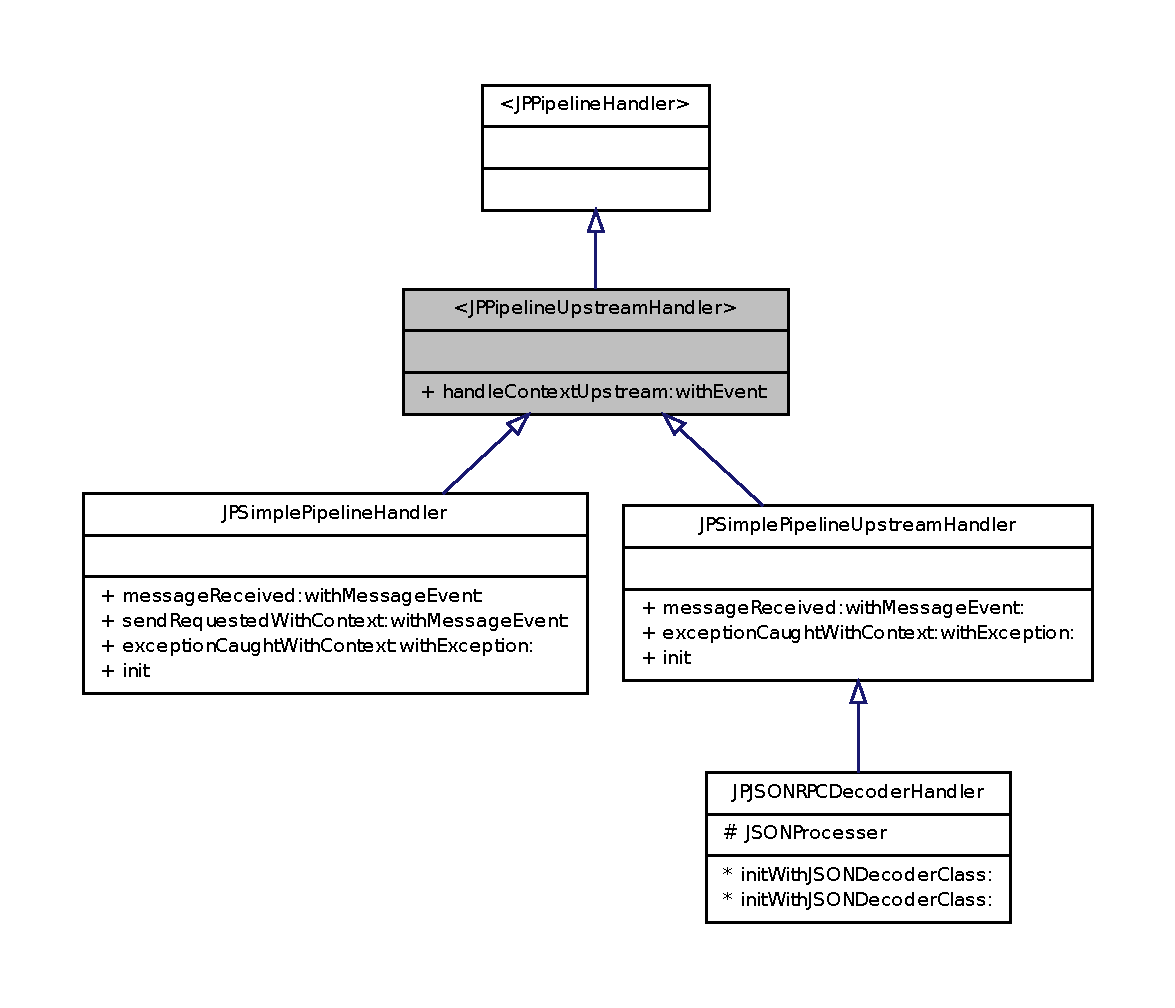
\includegraphics[width=400pt]{a00152}
\end{center}
\end{figure}


Collaboration diagram for $<$JPPipelineUpstreamHandler$>$:\nopagebreak
\begin{figure}[H]
\begin{center}
\leavevmode
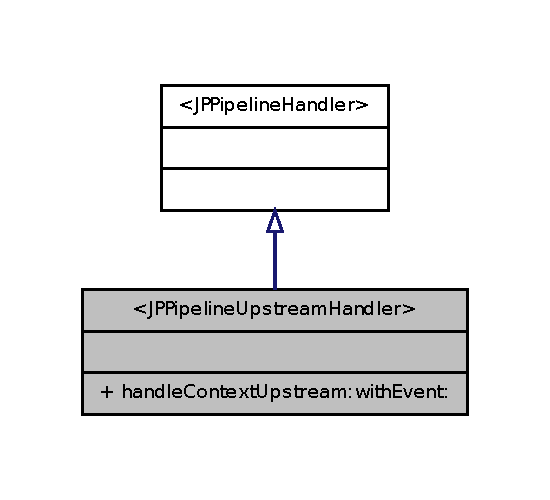
\includegraphics[width=264pt]{a00153}
\end{center}
\end{figure}
\subsection*{Public Member Functions}
\begin{DoxyCompactItemize}
\item 
(void) -\/ \hyperlink{a00035_ae561c9fac754928ec4e2bf253c7418d0}{handleContextUpstream:withEvent:}
\begin{DoxyCompactList}\small\item\em Handles the specified specified event. \item\end{DoxyCompactList}\end{DoxyCompactItemize}


\subsection{Detailed Description}
Handles or intercepts an upstream \hyperlink{a00023}{JPPipelineEvent}, and sends a \hyperlink{a00023}{JPPipelineEvent} to the next handler in a \hyperlink{a00019}{JPPipeline}. The most common use case of this interface is to intercept an event to transform the received messages or execute the relevant business logic.

\subsubsection*{Using the Upstream Handler Class}

In most cases, you will get to use a \hyperlink{a00039}{JPSimplePipelineUpstreamHandler} to implement an upstream handler because it provides an individual handler method for each event type. You might want to implement this interface directly though if you want to handle various types of events in more generic way.

\paragraph*{Firing an event to the next handler}

You can forward the received event upstream or downstream. In most cases, \hyperlink{a00035}{JPPipelineUpstreamHandler} will send the event upstream (i.e. inbound) although it is legal to send the event downstream (i.e. outbound):


\begin{DoxyCode}
 // Sending the event upstream (inbound)
 // Override...
 -(void)handleContextUpstream:(JPDefaultHandlerContext*)ctx withEvent:(<
      JPPipelineEvent>)e {
         ...
         [ctx sendUpstream:e];
         ...
 }
 
 // Sending the event downstream (outbound)
  -(void)handleContextDownstream:(JPDefaultHandlerContext*)ctx withEvent:(<
      JPPipelineEvent>)e {
         ...
         [ctx sendDownstream:[DownstreamMessageEvent init(...)]];
         ...
 }
\end{DoxyCode}
 

\subsection{Member Function Documentation}
\hypertarget{a00035_ae561c9fac754928ec4e2bf253c7418d0}{
\index{JPPipelineUpstreamHandler-\/p@{JPPipelineUpstreamHandler-\/p}!handleContextUpstream:withEvent:@{handleContextUpstream:withEvent:}}
\index{handleContextUpstream:withEvent:@{handleContextUpstream:withEvent:}!JPPipelineUpstreamHandler-p@{JPPipelineUpstreamHandler-\/p}}
\subsubsection[{handleContextUpstream:withEvent:}]{\setlength{\rightskip}{0pt plus 5cm}-\/ (void) handleContextUpstream: 
\begin{DoxyParamCaption}
\item[{dummy({\bf JPDefaultHandlerContext} $\ast$)}]{ctx}
\item[{withEvent:($<$ {\bf JPPipelineEvent} $>$)}]{e}
\end{DoxyParamCaption}
}}
\label{a00035_ae561c9fac754928ec4e2bf253c7418d0}


Handles the specified specified event. 


\begin{DoxyParams}{Parameters}
{\em ctx} & The context object for this handler. \\
\hline
{\em e} & The downstream event to process or intercept. \\
\hline
\end{DoxyParams}


The documentation for this protocol was generated from the following file:\begin{DoxyCompactItemize}
\item 
/Users/Paulo/Projects/JUMP/JUMPNetwork/Headers/JPPipelineUpstreamHandler.h\end{DoxyCompactItemize}

\hypertarget{a00036}{
\section{JPPipelineUpstreamMessageEvent Class Reference}
\label{a00036}\index{JPPipelineUpstreamMessageEvent@{JPPipelineUpstreamMessageEvent}}
}


The default Upstream Message Event implementation.  




{\ttfamily \#import $<$JPPipelineUpstreamMessageEvent.h$>$}



Inheritance diagram for JPPipelineUpstreamMessageEvent:\nopagebreak
\begin{figure}[H]
\begin{center}
\leavevmode
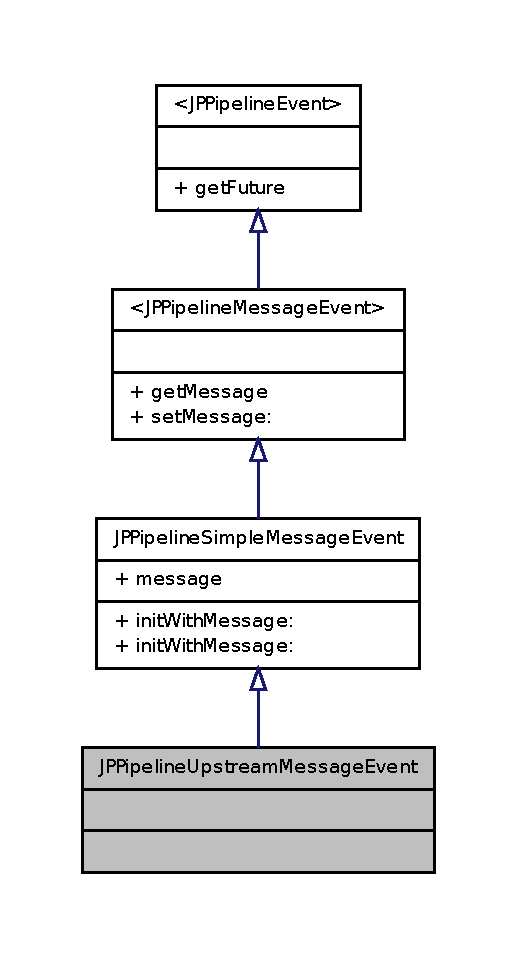
\includegraphics[width=248pt]{a00155}
\end{center}
\end{figure}


Collaboration diagram for JPPipelineUpstreamMessageEvent:\nopagebreak
\begin{figure}[H]
\begin{center}
\leavevmode
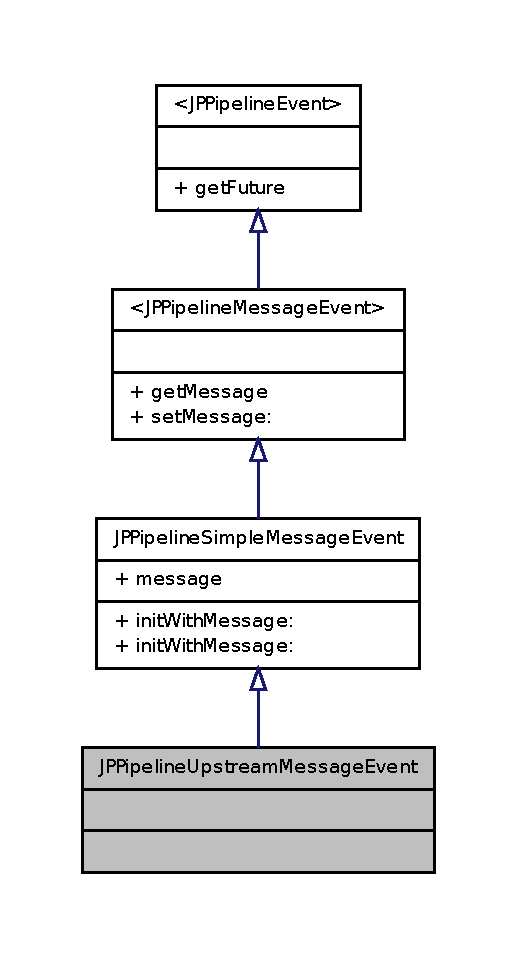
\includegraphics[width=248pt]{a00156}
\end{center}
\end{figure}


\subsection{Detailed Description}
The default Upstream Message Event implementation. 

The documentation for this class was generated from the following file:\begin{DoxyCompactItemize}
\item 
/Users/Paulo/Projects/JUMP/JUMPNetwork/Headers/JPPipelineUpstreamMessageEvent.h\end{DoxyCompactItemize}

\hypertarget{a00037}{
\section{JPSimplePipelineDownstreamHandler Class Reference}
\label{a00037}\index{JPSimplePipelineDownstreamHandler@{JPSimplePipelineDownstreamHandler}}
}


A \hyperlink{a00021}{JPPipelineDownstreamHandler} implementation which provides an individual handler method for each event type.  




{\ttfamily \#import $<$JPSimplePipelineDownstreamHandler.h$>$}



Inheritance diagram for JPSimplePipelineDownstreamHandler:\nopagebreak
\begin{figure}[H]
\begin{center}
\leavevmode
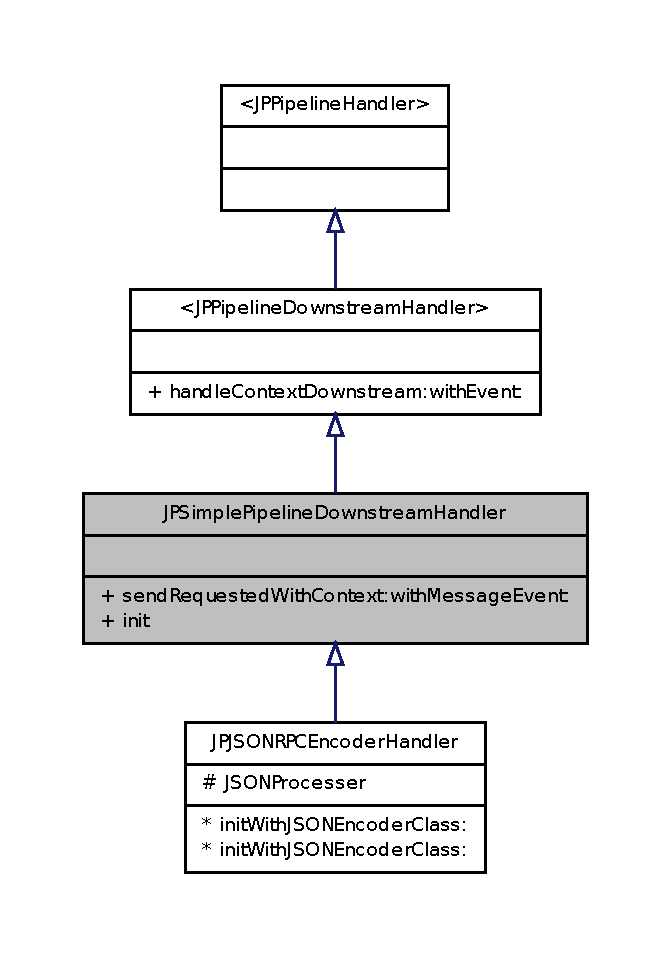
\includegraphics[width=322pt]{a00158}
\end{center}
\end{figure}


Collaboration diagram for JPSimplePipelineDownstreamHandler:\nopagebreak
\begin{figure}[H]
\begin{center}
\leavevmode
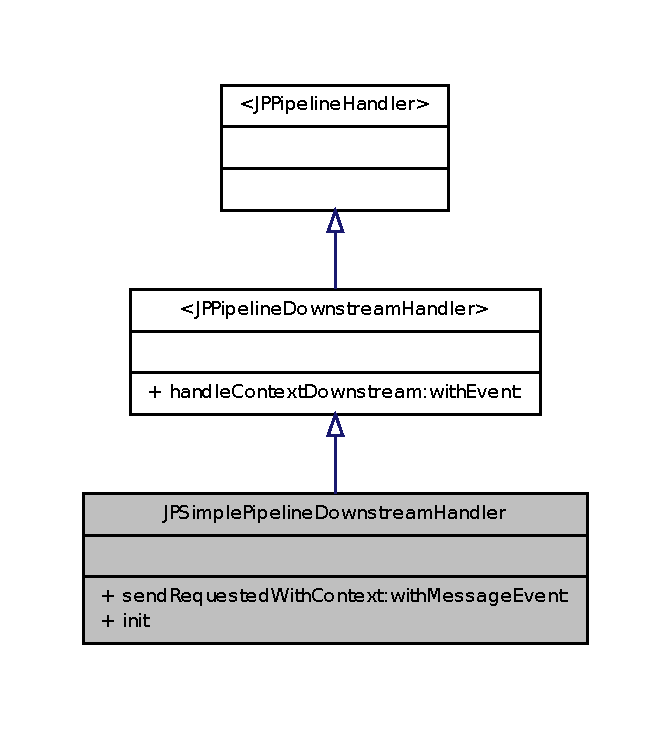
\includegraphics[width=322pt]{a00159}
\end{center}
\end{figure}
\subsection*{Public Member Functions}
\begin{DoxyCompactItemize}
\item 
(void) -\/ \hyperlink{a00037_a609e49c4f7c71002a13003112c2f6349}{sendRequestedWithContext:withMessageEvent:}
\begin{DoxyCompactList}\small\item\em Invoked when some Send data is requested. \item\end{DoxyCompactList}\end{DoxyCompactItemize}
\subsection*{Static Public Member Functions}
\begin{DoxyCompactItemize}
\item 
\hypertarget{a00037_abb497c02fc2f0a33f471a4c88d623205}{
(id) + \hyperlink{a00037_abb497c02fc2f0a33f471a4c88d623205}{init}}
\label{a00037_abb497c02fc2f0a33f471a4c88d623205}

\begin{DoxyCompactList}\small\item\em Init this handler. \item\end{DoxyCompactList}\end{DoxyCompactItemize}


\subsection{Detailed Description}
A \hyperlink{a00021}{JPPipelineDownstreamHandler} implementation which provides an individual handler method for each event type. This handler down-\/casts the received upstream event into more meaningful sub-\/type event and calls an appropriate handler method with the down-\/cast event. The names of the methods are identical to the upstream event names, as introduced in the \hyperlink{a00023}{JPPipelineEvent} documentation.

Please use \hyperlink{a00038}{JPSimplePipelineHandler} if you need to implement both \hyperlink{a00035}{JPPipelineUpstreamHandler} and \hyperlink{a00021}{JPPipelineDownstreamHandler}.

\subsubsection*{Overriding the handleContextDownstream method}

You can override the {\bfseries handleContextDownstream:withEvent:} method just like overriding an ordinary Objective-\/C method. Please make sure to call {\bfseries super} so that other handler methods are invoked properly:


\begin{DoxyCode}
 // Override...
 -(void)handleContextDownstream:(JPDefaultHandlerContext*)ctx withEvent:(<
      JPPipelineEvent>)e {
         ...
         [super handleContextDownstream:ctx withEvent:e];
         ...
 }
\end{DoxyCode}
 

\subsection{Member Function Documentation}
\hypertarget{a00037_a609e49c4f7c71002a13003112c2f6349}{
\index{JPSimplePipelineDownstreamHandler@{JPSimplePipelineDownstreamHandler}!sendRequestedWithContext:withMessageEvent:@{sendRequestedWithContext:withMessageEvent:}}
\index{sendRequestedWithContext:withMessageEvent:@{sendRequestedWithContext:withMessageEvent:}!JPSimplePipelineDownstreamHandler@{JPSimplePipelineDownstreamHandler}}
\subsubsection[{sendRequestedWithContext:withMessageEvent:}]{\setlength{\rightskip}{0pt plus 5cm}-\/ (void) sendRequestedWithContext: 
\begin{DoxyParamCaption}
\item[{dummy($<$ {\bf JPPipelineHandlerContext} $>$)}]{ctx}
\item[{withMessageEvent:($<$ {\bf JPPipelineMessageEvent} $>$)}]{e}
\end{DoxyParamCaption}
}}
\label{a00037_a609e49c4f7c71002a13003112c2f6349}


Invoked when some Send data is requested. 


\begin{DoxyParams}{Parameters}
{\em ctx} & An context. \\
\hline
{\em e} & The event. \\
\hline
\end{DoxyParams}


The documentation for this class was generated from the following file:\begin{DoxyCompactItemize}
\item 
/Users/Paulo/Projects/JUMP/JUMPNetwork/Headers/JPSimplePipelineDownstreamHandler.h\end{DoxyCompactItemize}

\hypertarget{a00038}{
\section{JPSimplePipelineHandler Class Reference}
\label{a00038}\index{JPSimplePipelineHandler@{JPSimplePipelineHandler}}
}


A \hyperlink{a00029}{JPPipelineHandler} which provides an individual handler method for each event type.  




{\ttfamily \#import $<$JPSimplePipelineHandler.h$>$}



Inheritance diagram for JPSimplePipelineHandler:\nopagebreak
\begin{figure}[H]
\begin{center}
\leavevmode
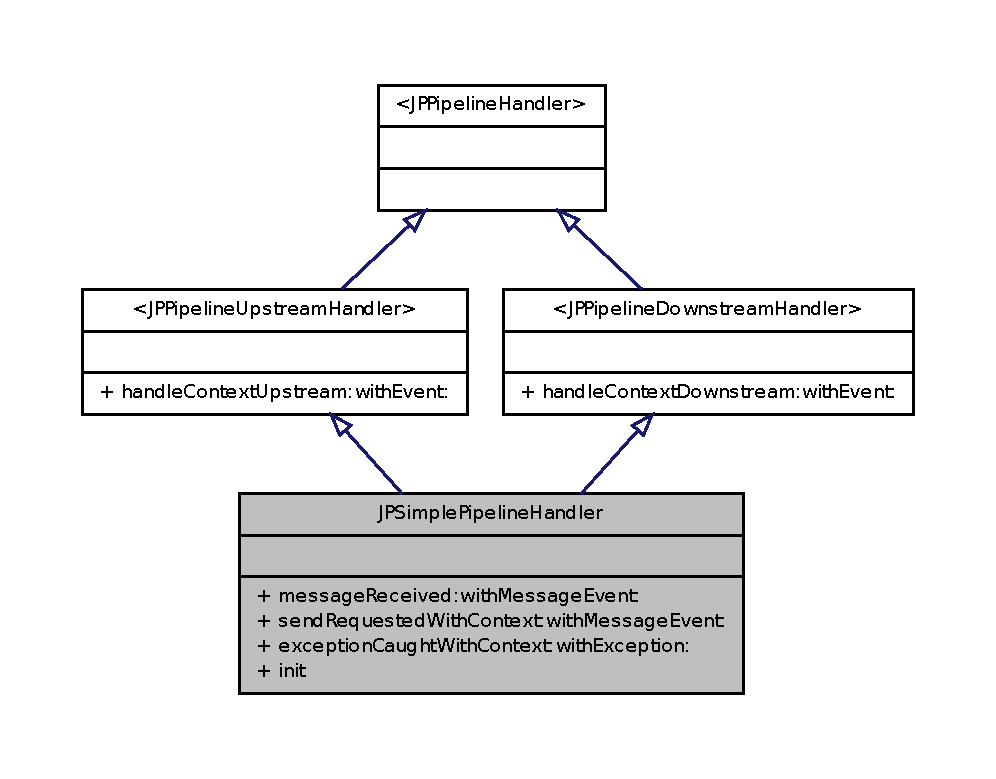
\includegraphics[width=400pt]{a00161}
\end{center}
\end{figure}


Collaboration diagram for JPSimplePipelineHandler:\nopagebreak
\begin{figure}[H]
\begin{center}
\leavevmode
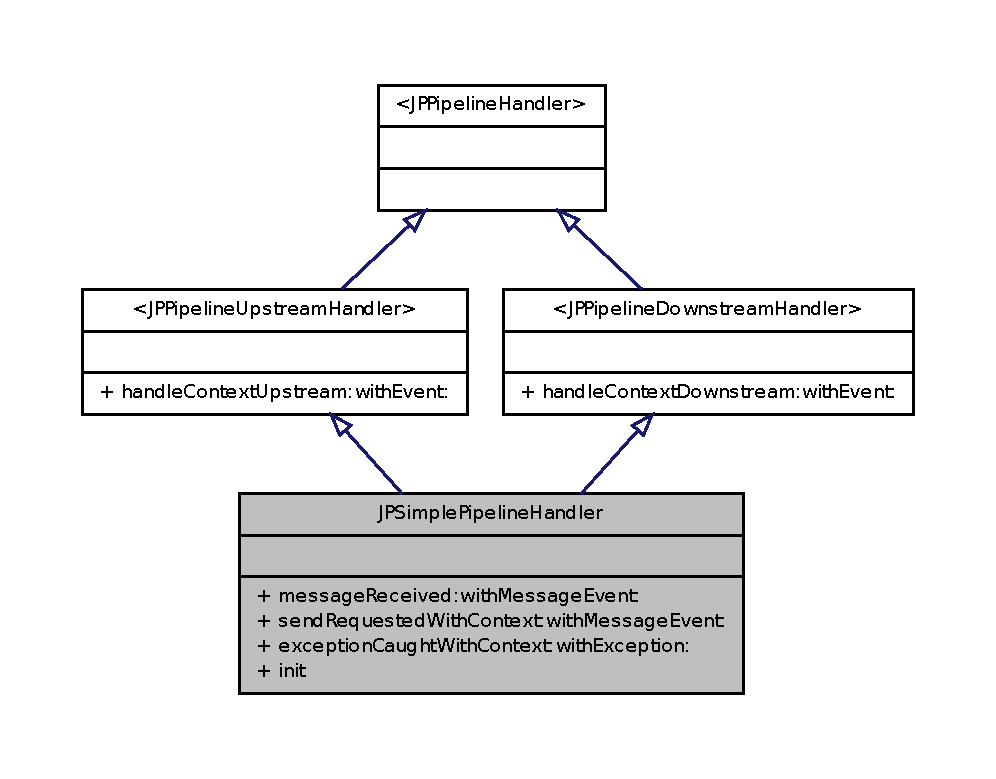
\includegraphics[width=400pt]{a00162}
\end{center}
\end{figure}
\subsection*{Public Member Functions}
\begin{DoxyCompactItemize}
\item 
(void) -\/ \hyperlink{a00038_ab7563b8931ff4b65d1419757748dbf86}{messageReceived:withMessageEvent:}
\begin{DoxyCompactList}\small\item\em Invoked when a message object was received. \item\end{DoxyCompactList}\item 
(void) -\/ \hyperlink{a00038_a4ea48ce584b89c8c2c611833a8da18ee}{sendRequestedWithContext:withMessageEvent:}
\begin{DoxyCompactList}\small\item\em Invoked when some Send data is requested. \item\end{DoxyCompactList}\item 
(void) -\/ \hyperlink{a00038_aa349318a897432c440c54ee2483d9e6c}{exceptionCaughtWithContext:withException:}
\begin{DoxyCompactList}\small\item\em Invoked when an exception was raised. \item\end{DoxyCompactList}\end{DoxyCompactItemize}
\subsection*{Static Public Member Functions}
\begin{DoxyCompactItemize}
\item 
\hypertarget{a00038_a0b2e233df8e8b95d1e2bbbc9cee8766e}{
(id) + \hyperlink{a00038_a0b2e233df8e8b95d1e2bbbc9cee8766e}{init}}
\label{a00038_a0b2e233df8e8b95d1e2bbbc9cee8766e}

\begin{DoxyCompactList}\small\item\em Init this handler. \item\end{DoxyCompactList}\end{DoxyCompactItemize}


\subsection{Detailed Description}
A \hyperlink{a00029}{JPPipelineHandler} which provides an individual handler method for each event type. This handler down-\/casts the received upstream or or downstream event into more meaningful sub-\/type event and calls an appropriate handler method with the down-\/cast event. For an upstream event, the names of the methods are identical to the upstream event names, as introduced in the \hyperlink{a00023}{JPPipelineEvent} documentation.

For a downstream event, the names of the methods starts with the name of the operation and ends with \char`\"{}Requested\char`\"{} (e.g. writeRequested.)

Please use \hyperlink{a00039}{JPSimplePipelineUpstreamHandler} or \hyperlink{a00037}{JPSimplePipelineDownstreamHandler} if you want to intercept only upstream or downstream events.

\subsubsection*{Overriding the handleContextUpstream and handleContextDownstream method}

You can override the {\bfseries handleContextUpstream:withEvent:} and {\bfseries handleContextDownstream:withEvent:} method just like overriding an ordinary Objective-\/C method. Please make sure to call {\bfseries super} so that other handler methods are invoked properly:


\begin{DoxyCode}
 // Override...
 -(void)handleContextUpstream:(JPDefaultHandlerContext*)ctx withEvent:(<
      JPPipelineEvent>)e {
         ...
         [super handleContextUpstream:ctx withEvent:e];
         ...
 }
 
 // Override...
 -(void)handleContextDownstream:(JPDefaultHandlerContext*)ctx withEvent:(<
      JPPipelineEvent>)e {
         ...
        [super handleContextDownstream:ctx withEvent:e];
         ...
 }
\end{DoxyCode}
 

\subsection{Member Function Documentation}
\hypertarget{a00038_ab7563b8931ff4b65d1419757748dbf86}{
\index{JPSimplePipelineHandler@{JPSimplePipelineHandler}!messageReceived:withMessageEvent:@{messageReceived:withMessageEvent:}}
\index{messageReceived:withMessageEvent:@{messageReceived:withMessageEvent:}!JPSimplePipelineHandler@{JPSimplePipelineHandler}}
\subsubsection[{messageReceived:withMessageEvent:}]{\setlength{\rightskip}{0pt plus 5cm}-\/ (void) messageReceived: 
\begin{DoxyParamCaption}
\item[{dummy($<$ {\bf JPPipelineHandlerContext} $>$)}]{ctx}
\item[{withMessageEvent:($<$ {\bf JPPipelineMessageEvent} $>$)}]{e}
\end{DoxyParamCaption}
}}
\label{a00038_ab7563b8931ff4b65d1419757748dbf86}


Invoked when a message object was received. 


\begin{DoxyParams}{Parameters}
{\em ctx} & An context. \\
\hline
{\em e} & The event. \\
\hline
\end{DoxyParams}
\hypertarget{a00038_a4ea48ce584b89c8c2c611833a8da18ee}{
\index{JPSimplePipelineHandler@{JPSimplePipelineHandler}!sendRequestedWithContext:withMessageEvent:@{sendRequestedWithContext:withMessageEvent:}}
\index{sendRequestedWithContext:withMessageEvent:@{sendRequestedWithContext:withMessageEvent:}!JPSimplePipelineHandler@{JPSimplePipelineHandler}}
\subsubsection[{sendRequestedWithContext:withMessageEvent:}]{\setlength{\rightskip}{0pt plus 5cm}-\/ (void) sendRequestedWithContext: 
\begin{DoxyParamCaption}
\item[{dummy($<$ {\bf JPPipelineHandlerContext} $>$)}]{ctx}
\item[{withMessageEvent:($<$ {\bf JPPipelineMessageEvent} $>$)}]{e}
\end{DoxyParamCaption}
}}
\label{a00038_a4ea48ce584b89c8c2c611833a8da18ee}


Invoked when some Send data is requested. 


\begin{DoxyParams}{Parameters}
{\em ctx} & An context. \\
\hline
{\em e} & The event. \\
\hline
\end{DoxyParams}
\hypertarget{a00038_aa349318a897432c440c54ee2483d9e6c}{
\index{JPSimplePipelineHandler@{JPSimplePipelineHandler}!exceptionCaughtWithContext:withException:@{exceptionCaughtWithContext:withException:}}
\index{exceptionCaughtWithContext:withException:@{exceptionCaughtWithContext:withException:}!JPSimplePipelineHandler@{JPSimplePipelineHandler}}
\subsubsection[{exceptionCaughtWithContext:withException:}]{\setlength{\rightskip}{0pt plus 5cm}-\/ (void) exceptionCaughtWithContext: 
\begin{DoxyParamCaption}
\item[{dummy($<$ {\bf JPPipelineHandlerContext} $>$)}]{ctx}
\item[{withException:($<$ {\bf JPPipelineExceptionEvent} $>$)}]{e}
\end{DoxyParamCaption}
}}
\label{a00038_aa349318a897432c440c54ee2483d9e6c}


Invoked when an exception was raised. 


\begin{DoxyParams}{Parameters}
{\em ctx} & An context. \\
\hline
{\em e} & The event. \\
\hline
\end{DoxyParams}


The documentation for this class was generated from the following file:\begin{DoxyCompactItemize}
\item 
/Users/Paulo/Projects/JUMP/JUMPNetwork/Headers/JPSimplePipelineHandler.h\end{DoxyCompactItemize}

\hypertarget{a00039}{
\section{JPSimplePipelineUpstreamHandler Class Reference}
\label{a00039}\index{JPSimplePipelineUpstreamHandler@{JPSimplePipelineUpstreamHandler}}
}


A \hyperlink{a00035}{JPPipelineUpstreamHandler} implementation which provides an individual handler method for each event type.  




{\ttfamily \#import $<$JPSimplePipelineUpstreamHandler.h$>$}



Inheritance diagram for JPSimplePipelineUpstreamHandler:\nopagebreak
\begin{figure}[H]
\begin{center}
\leavevmode
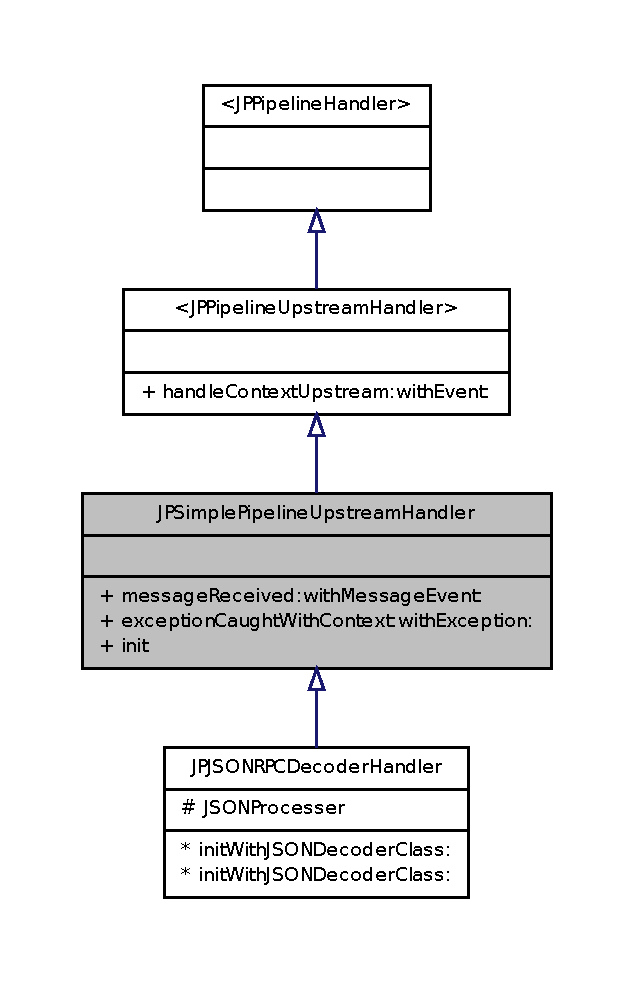
\includegraphics[width=304pt]{a00164}
\end{center}
\end{figure}


Collaboration diagram for JPSimplePipelineUpstreamHandler:\nopagebreak
\begin{figure}[H]
\begin{center}
\leavevmode
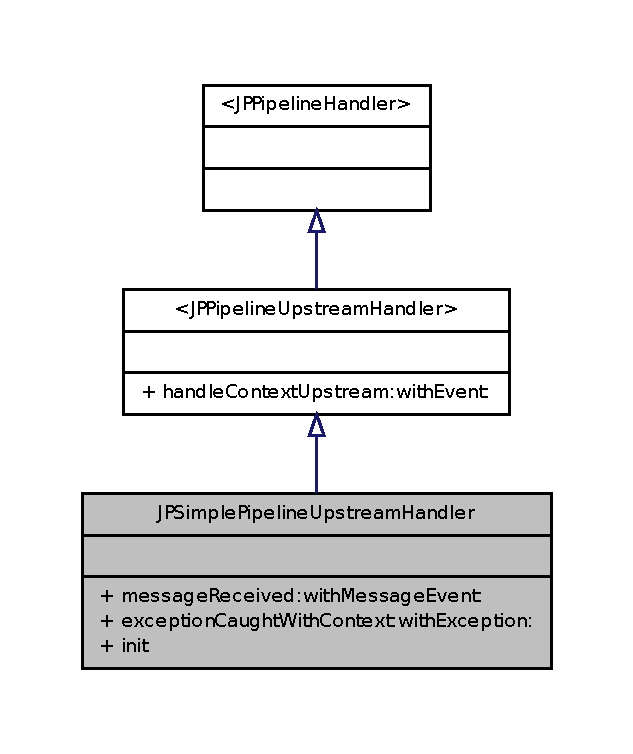
\includegraphics[width=304pt]{a00165}
\end{center}
\end{figure}
\subsection*{Public Member Functions}
\begin{DoxyCompactItemize}
\item 
(void) -\/ \hyperlink{a00039_ad4b20a4d32e1064cdeec4d0be6c17dd0}{messageReceived:withMessageEvent:}
\begin{DoxyCompactList}\small\item\em Invoked when a message object was received. \item\end{DoxyCompactList}\item 
(void) -\/ \hyperlink{a00039_a4c8e469d611291abdc56a79b7056a9ff}{exceptionCaughtWithContext:withException:}
\begin{DoxyCompactList}\small\item\em Invoked when an exception was raised. \item\end{DoxyCompactList}\end{DoxyCompactItemize}
\subsection*{Static Public Member Functions}
\begin{DoxyCompactItemize}
\item 
\hypertarget{a00039_aea40026cb9a22ff89738fc57510d8aa3}{
(id) + \hyperlink{a00039_aea40026cb9a22ff89738fc57510d8aa3}{init}}
\label{a00039_aea40026cb9a22ff89738fc57510d8aa3}

\begin{DoxyCompactList}\small\item\em Init this handler. \item\end{DoxyCompactList}\end{DoxyCompactItemize}


\subsection{Detailed Description}
A \hyperlink{a00035}{JPPipelineUpstreamHandler} implementation which provides an individual handler method for each event type. This handler down-\/casts the received upstream event into more meaningful sub-\/type event and calls an appropriate handler method with the down-\/cast event. The names of the methods are identical to the upstream event names, as introduced in the \hyperlink{a00023}{JPPipelineEvent} documentation.

Please use \hyperlink{a00038}{JPSimplePipelineHandler} if you need to implement both \hyperlink{a00035}{JPPipelineUpstreamHandler} and \hyperlink{a00021}{JPPipelineDownstreamHandler}.

\subsubsection*{Overriding the handleContextUpstream method}

You can override the {\bfseries handleContextUpstream:withEvent:} method just like overriding an ordinary Objective-\/C method. Please make sure to call {\bfseries super} so that other handler methods are invoked properly:


\begin{DoxyCode}
 // Override...
 -(void)handleContextUpstream:(JPDefaultHandlerContext*)ctx withEvent:(<
      JPPipelineEvent>)e {
         ...
         [super handleContextUpstream:ctx withEvent:e];
         ...
 }
\end{DoxyCode}
 

\subsection{Member Function Documentation}
\hypertarget{a00039_ad4b20a4d32e1064cdeec4d0be6c17dd0}{
\index{JPSimplePipelineUpstreamHandler@{JPSimplePipelineUpstreamHandler}!messageReceived:withMessageEvent:@{messageReceived:withMessageEvent:}}
\index{messageReceived:withMessageEvent:@{messageReceived:withMessageEvent:}!JPSimplePipelineUpstreamHandler@{JPSimplePipelineUpstreamHandler}}
\subsubsection[{messageReceived:withMessageEvent:}]{\setlength{\rightskip}{0pt plus 5cm}-\/ (void) messageReceived: 
\begin{DoxyParamCaption}
\item[{dummy($<$ {\bf JPPipelineHandlerContext} $>$)}]{ctx}
\item[{withMessageEvent:($<$ {\bf JPPipelineMessageEvent} $>$)}]{e}
\end{DoxyParamCaption}
}}
\label{a00039_ad4b20a4d32e1064cdeec4d0be6c17dd0}


Invoked when a message object was received. 


\begin{DoxyParams}{Parameters}
{\em ctx} & An context. \\
\hline
{\em e} & The event. \\
\hline
\end{DoxyParams}
\hypertarget{a00039_a4c8e469d611291abdc56a79b7056a9ff}{
\index{JPSimplePipelineUpstreamHandler@{JPSimplePipelineUpstreamHandler}!exceptionCaughtWithContext:withException:@{exceptionCaughtWithContext:withException:}}
\index{exceptionCaughtWithContext:withException:@{exceptionCaughtWithContext:withException:}!JPSimplePipelineUpstreamHandler@{JPSimplePipelineUpstreamHandler}}
\subsubsection[{exceptionCaughtWithContext:withException:}]{\setlength{\rightskip}{0pt plus 5cm}-\/ (void) exceptionCaughtWithContext: 
\begin{DoxyParamCaption}
\item[{dummy($<$ {\bf JPPipelineHandlerContext} $>$)}]{ctx}
\item[{withException:($<$ {\bf JPPipelineExceptionEvent} $>$)}]{e}
\end{DoxyParamCaption}
}}
\label{a00039_a4c8e469d611291abdc56a79b7056a9ff}


Invoked when an exception was raised. 


\begin{DoxyParams}{Parameters}
{\em ctx} & An context. \\
\hline
{\em e} & The event. \\
\hline
\end{DoxyParams}


The documentation for this class was generated from the following file:\begin{DoxyCompactItemize}
\item 
/Users/Paulo/Projects/JUMP/JUMPNetwork/Headers/JPSimplePipelineUpstreamHandler.h\end{DoxyCompactItemize}

\hypertarget{a00040}{
\section{$<$JPTransporterHTTPMessage$>$ Protocol Reference}
\label{a00040}\index{JPTransporterHTTPMessage-\/p@{JPTransporterHTTPMessage-\/p}}
}


\hyperlink{a00040}{JPTransporterHTTPMessage} is an special type of \hyperlink{a00005}{Event} that encapsulate the HTTP data to be transported.  




{\ttfamily \#import $<$JPTransporterHTTPMessage.h$>$}



Inheritance diagram for $<$JPTransporterHTTPMessage$>$:
\nopagebreak
\begin{figure}[H]
\begin{center}
\leavevmode
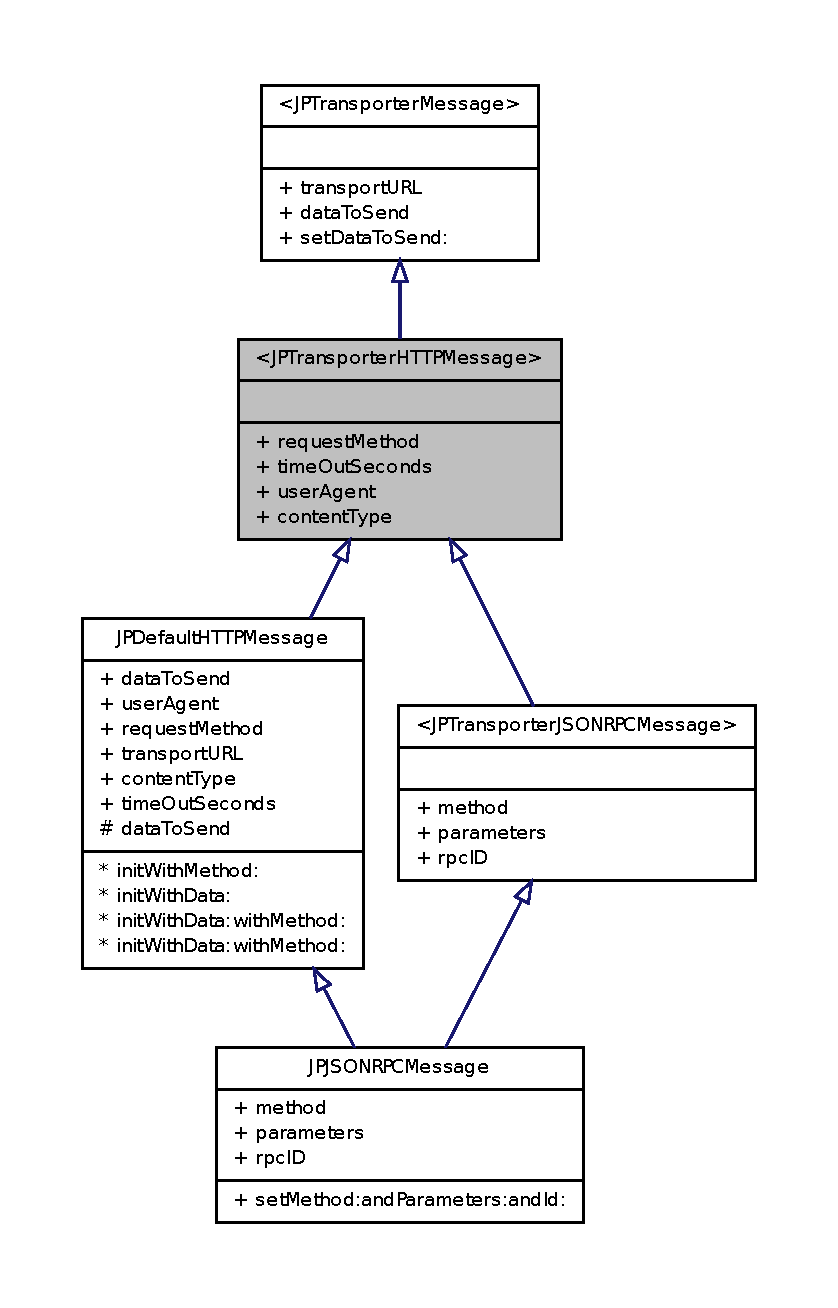
\includegraphics[height=600pt]{a00167}
\end{center}
\end{figure}


Collaboration diagram for $<$JPTransporterHTTPMessage$>$:\nopagebreak
\begin{figure}[H]
\begin{center}
\leavevmode
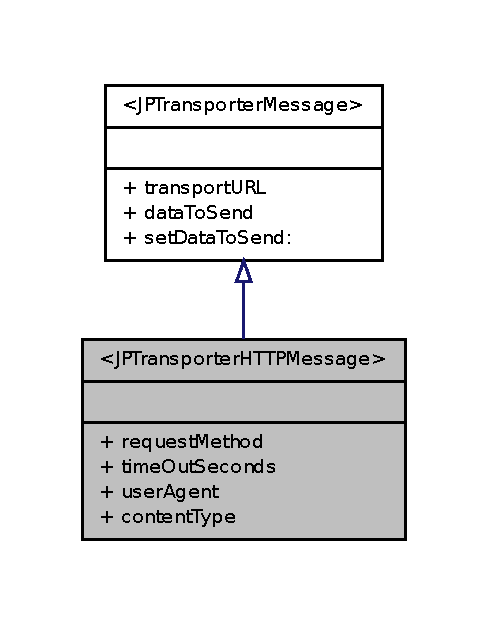
\includegraphics[width=234pt]{a00168}
\end{center}
\end{figure}
\subsection*{Public Member Functions}
\begin{DoxyCompactItemize}
\item 
\hypertarget{a00040_a0ed49760ae9138e2e7e5d7b8acde745b}{
(NSString $\ast$) -\/ \hyperlink{a00040_a0ed49760ae9138e2e7e5d7b8acde745b}{requestMethod}}
\label{a00040_a0ed49760ae9138e2e7e5d7b8acde745b}

\begin{DoxyCompactList}\small\item\em HTTP method to use (GET / POST / PUT / DELETE / HEAD). \item\end{DoxyCompactList}\item 
\hypertarget{a00040_a6d9652a819ac429e1c09b095d0424872}{
(NSTimeInterval) -\/ \hyperlink{a00040_a6d9652a819ac429e1c09b095d0424872}{timeOutSeconds}}
\label{a00040_a6d9652a819ac429e1c09b095d0424872}

\begin{DoxyCompactList}\small\item\em Number of seconds to wait before timing out. \item\end{DoxyCompactList}\item 
\hypertarget{a00040_a70431efd75f797fd2321dff4ed11499e}{
(NSString $\ast$) -\/ \hyperlink{a00040_a70431efd75f797fd2321dff4ed11499e}{userAgent}}
\label{a00040_a70431efd75f797fd2321dff4ed11499e}

\begin{DoxyCompactList}\small\item\em HTTP User Agent Identifier. \item\end{DoxyCompactList}\item 
\hypertarget{a00040_a2367186c814d6edbf34b085d2341f29c}{
(NSString $\ast$) -\/ \hyperlink{a00040_a2367186c814d6edbf34b085d2341f29c}{contentType}}
\label{a00040_a2367186c814d6edbf34b085d2341f29c}

\begin{DoxyCompactList}\small\item\em HTTP Content Type Identifier. \item\end{DoxyCompactList}\end{DoxyCompactItemize}


\subsection{Detailed Description}
\hyperlink{a00040}{JPTransporterHTTPMessage} is an special type of \hyperlink{a00005}{Event} that encapsulate the HTTP data to be transported. 

The documentation for this protocol was generated from the following file:\begin{DoxyCompactItemize}
\item 
/Users/Paulo/Projects/JUMP/JUMPNetwork/Headers/JPTransporterHTTPMessage.h\end{DoxyCompactItemize}

\hypertarget{a00041}{
\section{$<$JPTransporterJSONRPCMessage$>$ Protocol Reference}
\label{a00041}\index{JPTransporterJSONRPCMessage-\/p@{JPTransporterJSONRPCMessage-\/p}}
}


A Event which represent the JSON RPC Encapsulated Data.  




{\ttfamily \#import $<$JPTransporterJSONRPCMessage.h$>$}



Inheritance diagram for $<$JPTransporterJSONRPCMessage$>$:\nopagebreak
\begin{figure}[H]
\begin{center}
\leavevmode
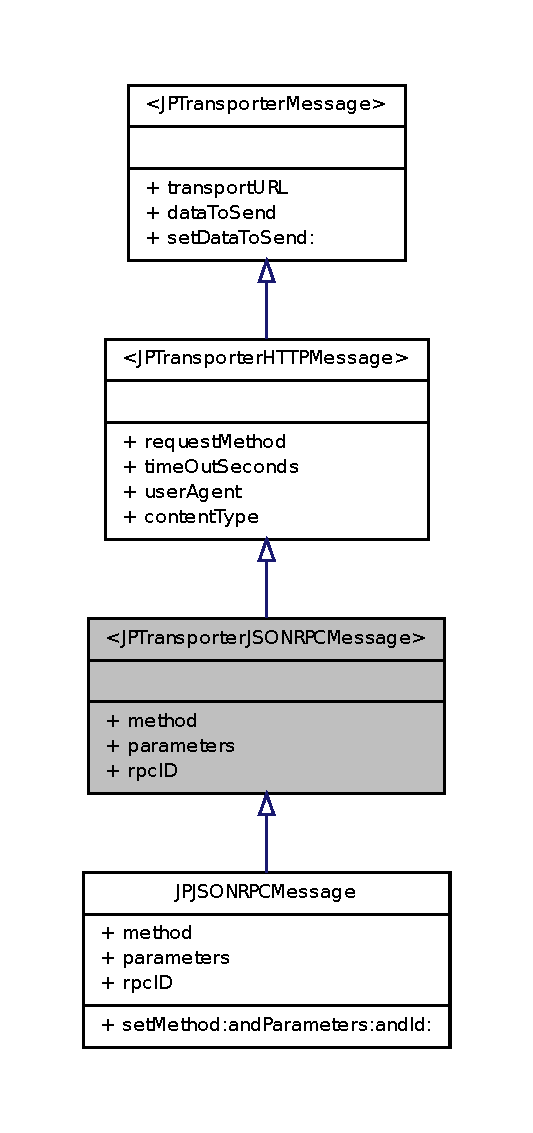
\includegraphics[width=256pt]{a00170}
\end{center}
\end{figure}


Collaboration diagram for $<$JPTransporterJSONRPCMessage$>$:\nopagebreak
\begin{figure}[H]
\begin{center}
\leavevmode
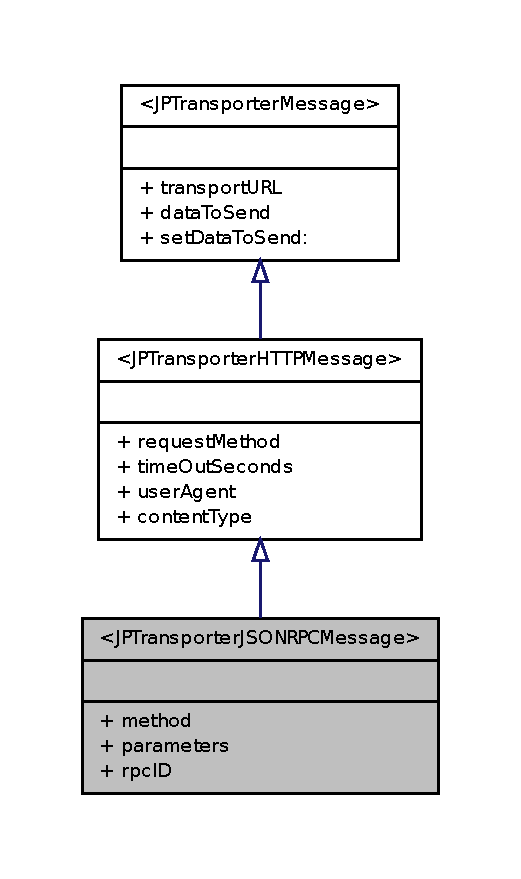
\includegraphics[width=250pt]{a00171}
\end{center}
\end{figure}
\subsection*{Public Member Functions}
\begin{DoxyCompactItemize}
\item 
\hypertarget{a00041_ade40198560090cabaf5b8a76b1d9af42}{
(NSString $\ast$) -\/ \hyperlink{a00041_ade40198560090cabaf5b8a76b1d9af42}{method}}
\label{a00041_ade40198560090cabaf5b8a76b1d9af42}

\begin{DoxyCompactList}\small\item\em JSON-\/RPC Method. \item\end{DoxyCompactList}\item 
\hypertarget{a00041_a32c1360e57655812c62599d5d1f9d5c3}{
(NSArray $\ast$) -\/ \hyperlink{a00041_a32c1360e57655812c62599d5d1f9d5c3}{parameters}}
\label{a00041_a32c1360e57655812c62599d5d1f9d5c3}

\begin{DoxyCompactList}\small\item\em JSON-\/RPC parameters. \item\end{DoxyCompactList}\item 
\hypertarget{a00041_aea883f630b43684c534ee095624d7226}{
(NSNumber $\ast$) -\/ \hyperlink{a00041_aea883f630b43684c534ee095624d7226}{rpcID}}
\label{a00041_aea883f630b43684c534ee095624d7226}

\begin{DoxyCompactList}\small\item\em JSON-\/RPC id. \item\end{DoxyCompactList}\end{DoxyCompactItemize}


\subsection{Detailed Description}
A Event which represent the JSON RPC Encapsulated Data. 

The documentation for this protocol was generated from the following file:\begin{DoxyCompactItemize}
\item 
/Users/Paulo/Projects/JUMP/JUMPNetwork/Headers/JPTransporterJSONRPCMessage.h\end{DoxyCompactItemize}

\hypertarget{a00042}{
\section{$<$JPTransporterMessage$>$ Protocol Reference}
\label{a00042}\index{JPTransporterMessage-\/p@{JPTransporterMessage-\/p}}
}


A Event which represent the fundamental information to the \hyperlink{a00002}{I$|$O Transporter}.  




{\ttfamily \#import $<$JPTransporterMessage.h$>$}



Inheritance diagram for $<$JPTransporterMessage$>$:
\nopagebreak
\begin{figure}[H]
\begin{center}
\leavevmode
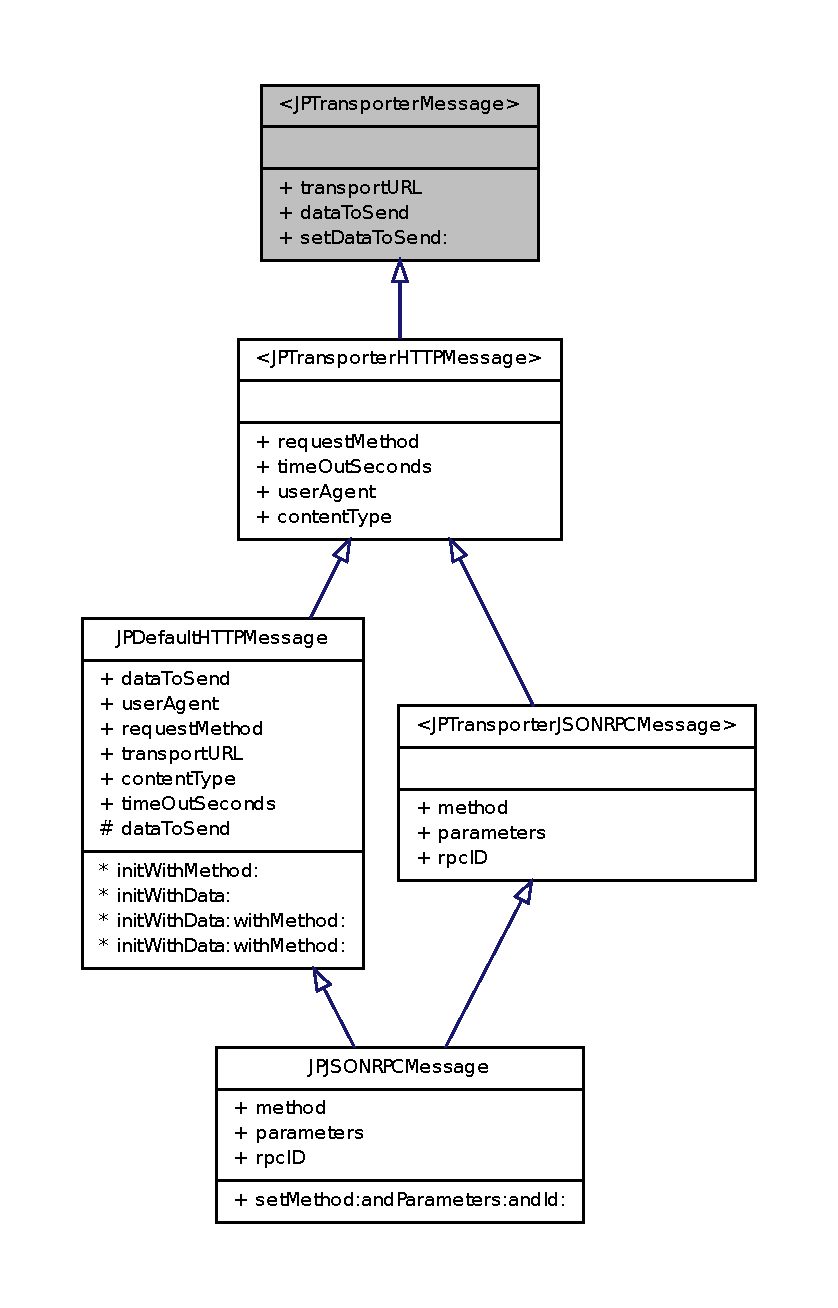
\includegraphics[height=600pt]{a00173}
\end{center}
\end{figure}
\subsection*{Public Member Functions}
\begin{DoxyCompactItemize}
\item 
\hypertarget{a00042_a8832d16762be0fa91050304e2d72ebe0}{
(NSURL $\ast$) -\/ \hyperlink{a00042_a8832d16762be0fa91050304e2d72ebe0}{transportURL}}
\label{a00042_a8832d16762be0fa91050304e2d72ebe0}

\begin{DoxyCompactList}\small\item\em Returns the URL to connect and communicate. \item\end{DoxyCompactList}\item 
\hypertarget{a00042_a3bdde47fa8f94d7ed8237b8985808616}{
(NSData $\ast$) -\/ \hyperlink{a00042_a3bdde47fa8f94d7ed8237b8985808616}{dataToSend}}
\label{a00042_a3bdde47fa8f94d7ed8237b8985808616}

\begin{DoxyCompactList}\small\item\em Data to transport. \item\end{DoxyCompactList}\item 
\hypertarget{a00042_acabee3cab759c235f5a719b059c1d752}{
(void) -\/ \hyperlink{a00042_acabee3cab759c235f5a719b059c1d752}{setDataToSend:}}
\label{a00042_acabee3cab759c235f5a719b059c1d752}

\begin{DoxyCompactList}\small\item\em Set Data to transport. \item\end{DoxyCompactList}\end{DoxyCompactItemize}


\subsection{Detailed Description}
A Event which represent the fundamental information to the \hyperlink{a00002}{I$|$O Transporter}. 

The documentation for this protocol was generated from the following file:\begin{DoxyCompactItemize}
\item 
/Users/Paulo/Projects/JUMP/JUMPNetwork/Headers/JPTransporterMessage.h\end{DoxyCompactItemize}

\printindex
\end{document}
